%========================================================
\section{Legacy Examples}\label{sec:legacyexamples}
%========================================================

% start with section 0
\setcounter{subsection}{-1}
\subsection{ORE Web Service}\label{sec:service}

Since release 12, ORE comes with a proof-of-concept implementation of a web service around ORE
that is written in Python, see folder {\tt Examples/API}.

The service is based on
\begin{itemize}
\item the flask web framework \url{https://flask.palletsprojects.com}, and
\item the ORE Python module which can be installed using \\
  {\tt pip install open-source-risk-engine} \\
  or built from sources following the instructions in the ORE-SWIG repository
  at \url{https://github.com/opensourcerisk/ore-swig}.
\end{itemize}

\medskip
Main files in the {\tt Examples/API} directory:
\begin{itemize}
\item {\bf restapi.py} runs a flask api as analytics service that takes a post request
  (e.g. from a server like postman, or from a python script): The request contains a json body
  which corresponds to the data usually contained in the master input file ore.xml. restapi.py
  calls the oreApi.py class (see below) to do the work. By default, the analytics service listens for
  requests on port 5001.
\item {\bf oreApi.py} reads the json body, compiles all ORE input parameters, calls into a
  data service (see below) to retrieve additional data. Then it kicks off an ORE run to process
  the request.  Finally it posts resulting reports through the data service.
\item {\bf simplefileserver.py} runs a flask api as a data service. It takes requests from the
  analytics service above in the form of urls of xml files that contain additional data required
  by ORE (market data, portfolio, configuration). By default, the data service
  listens on port 5000, reads from the Input directory in Examples/API and writes reports to the Output
  directory in Examples/API.
\end{itemize}

\medskip
Run a local example:
\begin{itemize}
\item start the data service: \\
  {\tt python3 simplefileserver.py \&} 
\item start the analytics service: \\
  {\tt python3 restapi.py \&}
\item send a request to run the equivalent of Example 1: \\
  {\tt python3 request.py} \\
  Note that the json equivalent of {\tt Example\_1/Input/ore.xml} is contained in request.py,
  and all other inputs are retrieved from folder Examples/API/Input via the data service.
\end{itemize}

%See {\tt Examples/API/ReadMe.txt} for further ways to utilise the service, e.g. to run all
%examples in this section, deploy via docker etc.

%--------------------------------------------------------
\subsection{Interest Rate Swap Exposure, Flat Market}\label{sec:example1}
%--------------------------------------------------------

We start with a vanilla single currency Swap (currency EUR, maturity 20y, notional 10m, receive fixed 2\% annual, pay
6M-Euribor flat). The market yield curves (for both discounting and forward projection) are set to be flat at 2\% for
all maturities, i.e. the Swap is at the money initially and remains at the money on average throughout its life. Running
ORE in directory {\tt Examples/Example\_1} with

\medskip
\centerline{\tt python run.py } 
\medskip

yields the exposure evolution in 

\medskip
\centerline{\tt Examples/Example\_1/Output/*.pdf } 
\medskip

and shown in figure \ref{fig_1}. 
\begin{figure}[h!]
\begin{center}
%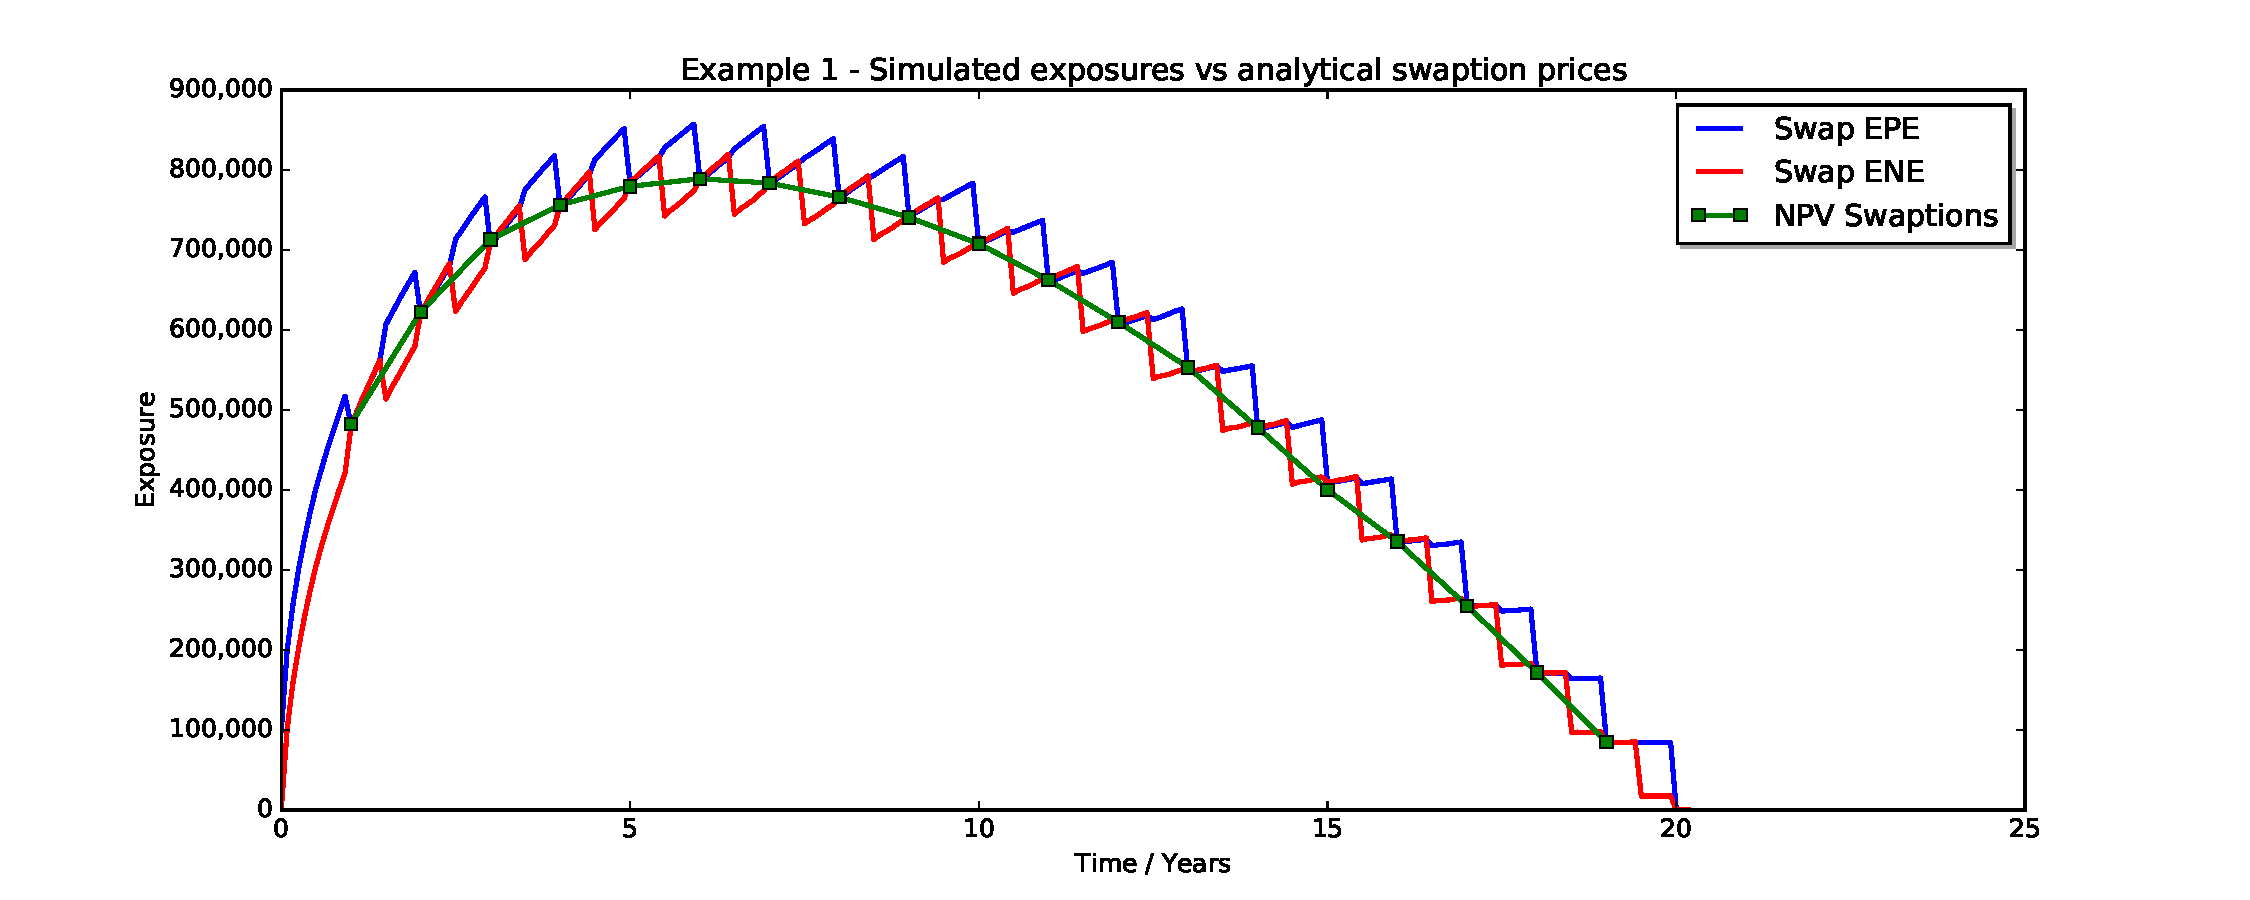
\includegraphics[scale=0.45]{mpl_swap_1_1m_sbb_100k.pdf}
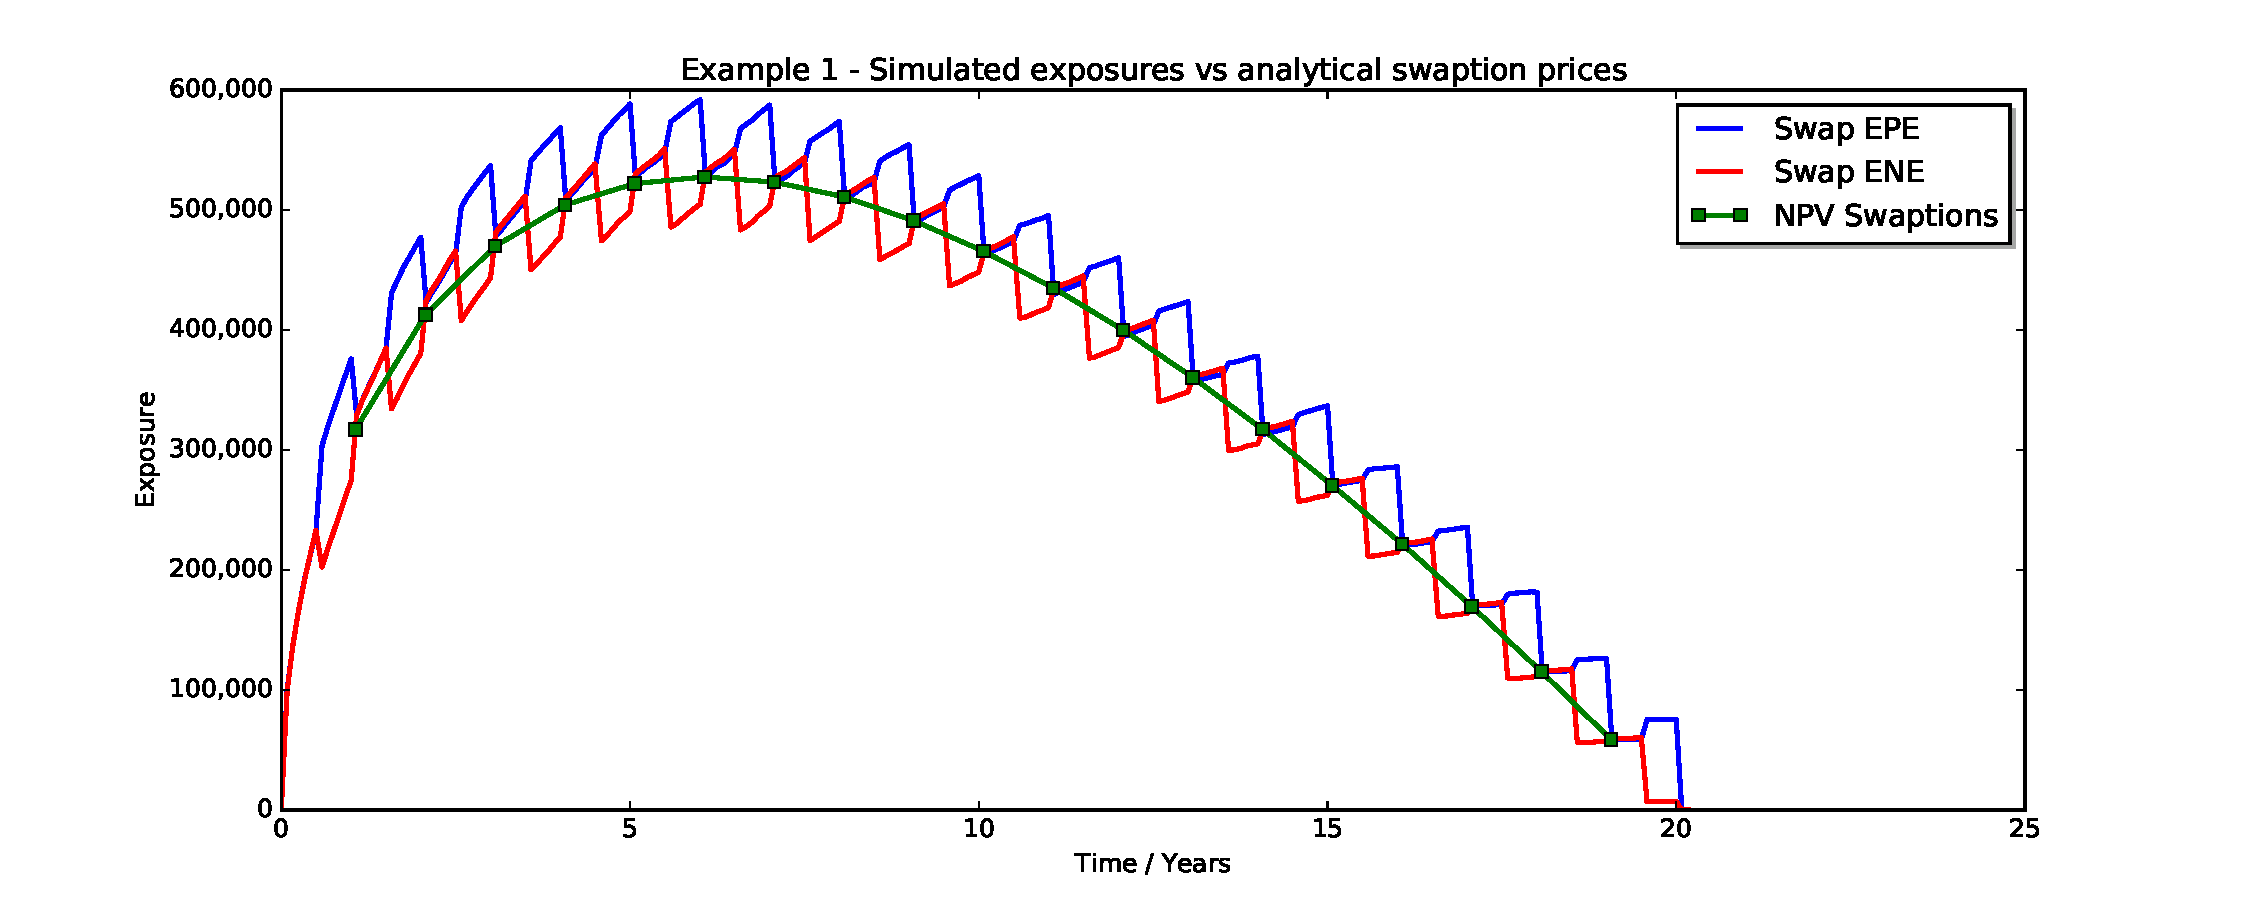
\includegraphics[scale=0.45]{examples/mpl_swap_1_1m_sbb_10k_flat.pdf}
\end{center}
\caption{Vanilla ATM Swap expected exposure in a flat market environment from both parties' perspectives. The symbols are European Swaption prices. The simulation was run with monthly time steps and 10,000 Monte Carlo samples to demonstrate the convergence of EPE and ENE profiles. A similar
outcome can be obtained more quickly with 5,000 samples on a quarterly time grid which is the default setting of Example\_1. }
\label{fig_1}
\end{figure}
Both Swap simulation and Swaption pricing are run with calls to the ORE executable, essentially 

\medskip
\centerline{\tt ore[.exe] ore.xml} 

\centerline{\tt ore[.exe] ore\_swaption.xml} 
\medskip

which are wrapped into the script {\tt Examples/Example\_1/run.py} provided with the ORE release.
It is instructive to look into the input folder in Examples/Example\_1, the content of the main input file {\tt
  ore.xml}, together with the explanations in section \ref{sec:configuration}. \\

This simple example is an important test case which is also run similarly in one of the unit test suites of ORE. The
expected exposure can be seen as a European option on the underlying netting set, see also \cite{methods}.
In this example, the expected exposure at some future point in time, say 10 years, is equal to
the European Swaption price for an option with expiry in 10 years, underlying Swap start in 10 years and underlying Swap
maturity in 20 years. We can easily compute such standard European Swaption prices for all future points in time where
both Swap legs reset, i.e. annually in this case\footnote{Using closed form expressions for standard European Swaption
  prices.}. And if the simulation model has been calibrated to the points on the Swaption surface which are used for
European Swaption pricing, then we can expect to see that the simulated exposure matches Swaption prices at these annual
points, as in figure \ref{fig_1}.  In Example\_1 we used co-terminal ATM Swaptions for both model calibration and
Swaption pricing. Moreover, as the yield curve is flat in this example, the exposures from both parties'
perspectives (EPE and ENE) match not only at the annual resets, but also for the period between annual reset of both
legs to the point in time when the floating leg resets. Thereafter, between floating leg (only) reset and next joint
fixed/floating leg reset, we see and expect a deviation of the two exposure profiles.

%--------------------------------------------------------
\subsection{Interest Rate Swap Exposure, Realistic Market}\label{sec:example2}
%--------------------------------------------------------

Moving to {\tt Examples/Example\_2}, we see what changes when using a realistic (non-flat) market
environment. Running the example with

\medskip
\centerline{\tt python run.py } 
\medskip

yields the exposure evolution in 

\medskip
\centerline{\tt Examples/Example\_2/Output/*.pdf } 
\medskip

shown in figure \ref{fig_2}.
\begin{figure}[h!]
\begin{center}
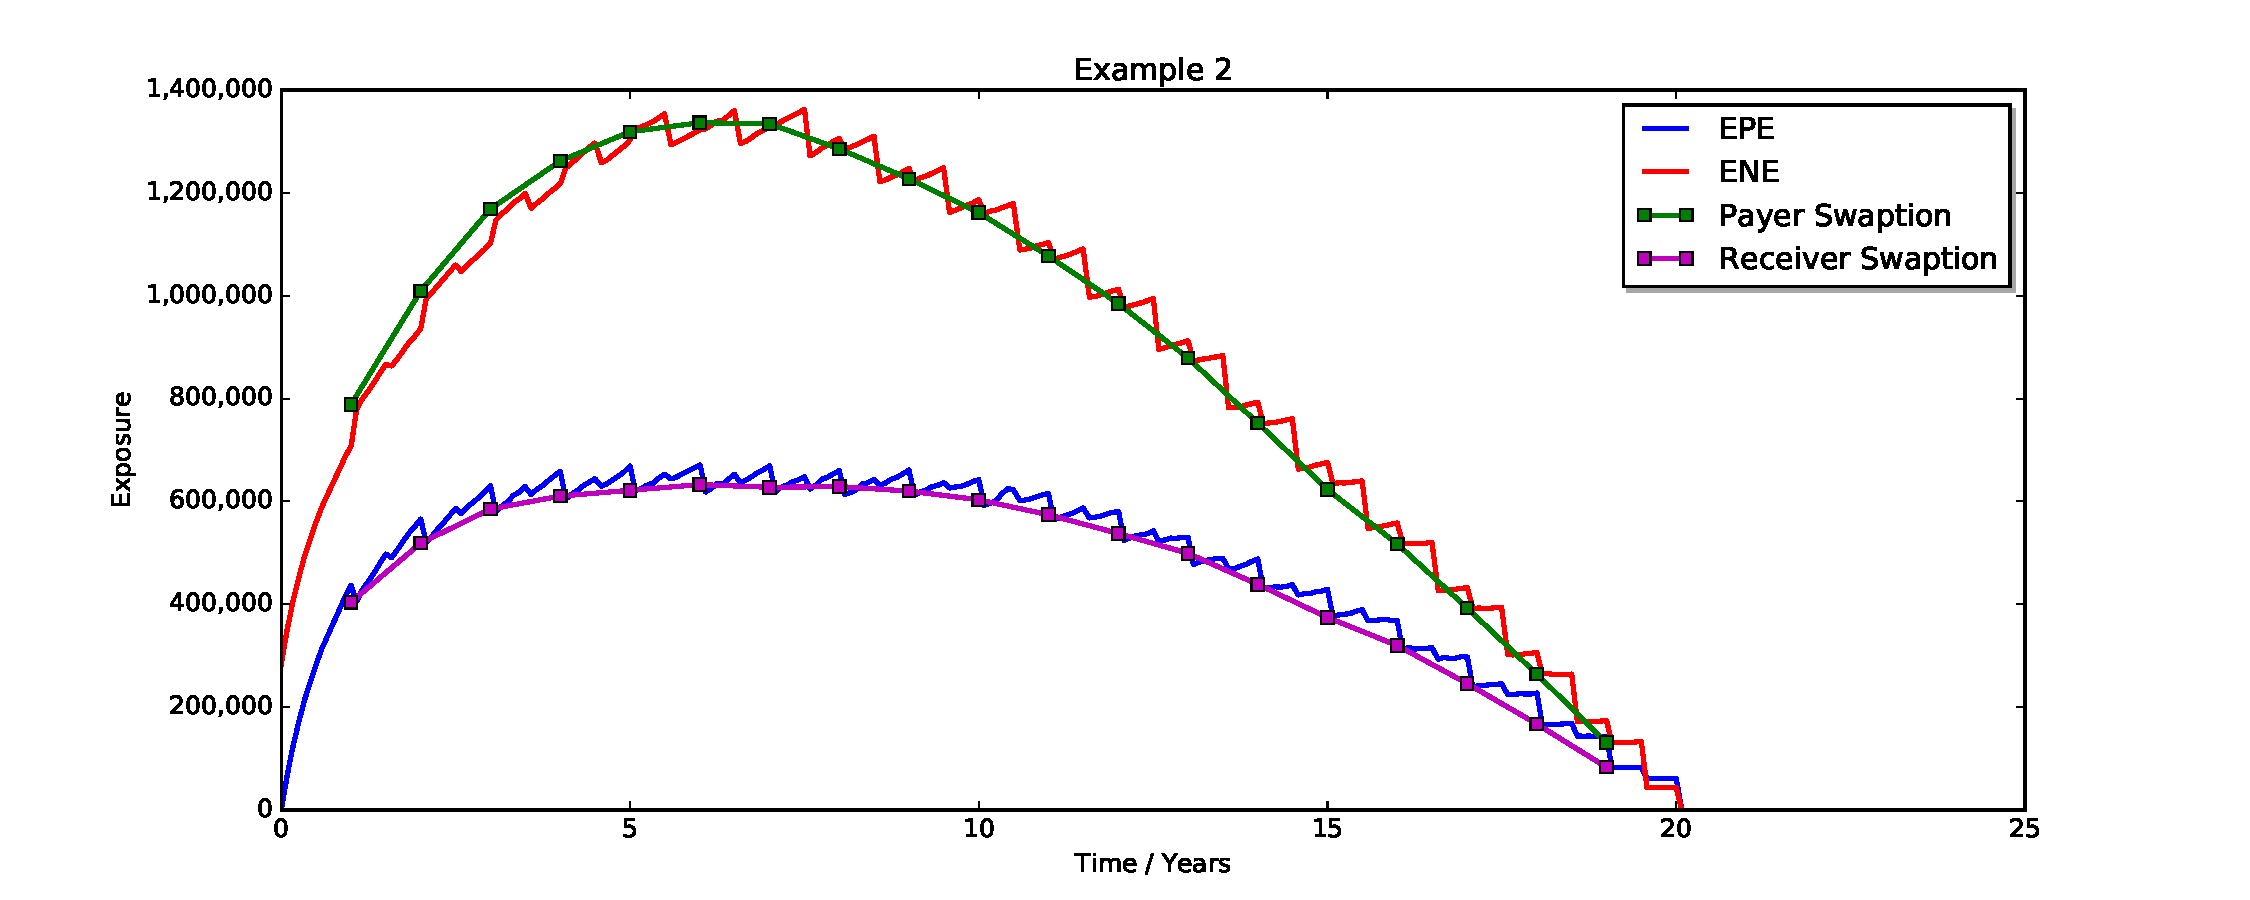
\includegraphics[scale=0.45]{examples/mpl_swap_3.pdf}
\end{center}
\caption{Vanilla ATM Swap expected exposure in a realistic market environment as of 05/02/2016 from both parties'
  perspectives. The Swap is the same as in figure \ref{fig_1} but receiving fixed 1\%, roughly at the money. The symbols
  are the prices of European payer and receiver Swaptions. Simulation with 5000 paths and monthly time steps.}
\label{fig_2}
\end{figure}
In this case, where the curves (discount and forward) are upward sloping, the receiver Swap is at the money at inception
only and moves (on average) out of the money during its life. Similarly, the Swap moves into the money from the
counterparty's perspective. Hence the expected exposure evolutions from our perspective (EPE) and the counterparty's
perspective (ENE) 'detach' here, while both can still be be reconciled with payer or respectively receiver Swaption
prices.

%--------------------------------------------------------
\subsection{European Swaption Exposure}\label{sec:european_swaption}
%--------------------------------------------------------

This demo case in folder {\tt Examples/Example\_3} shows the exposure evolution of European Swaptions with cash and
physical delivery, respectively, see figure \ref{fig_3}.
\begin{figure}[h!]
\begin{center}
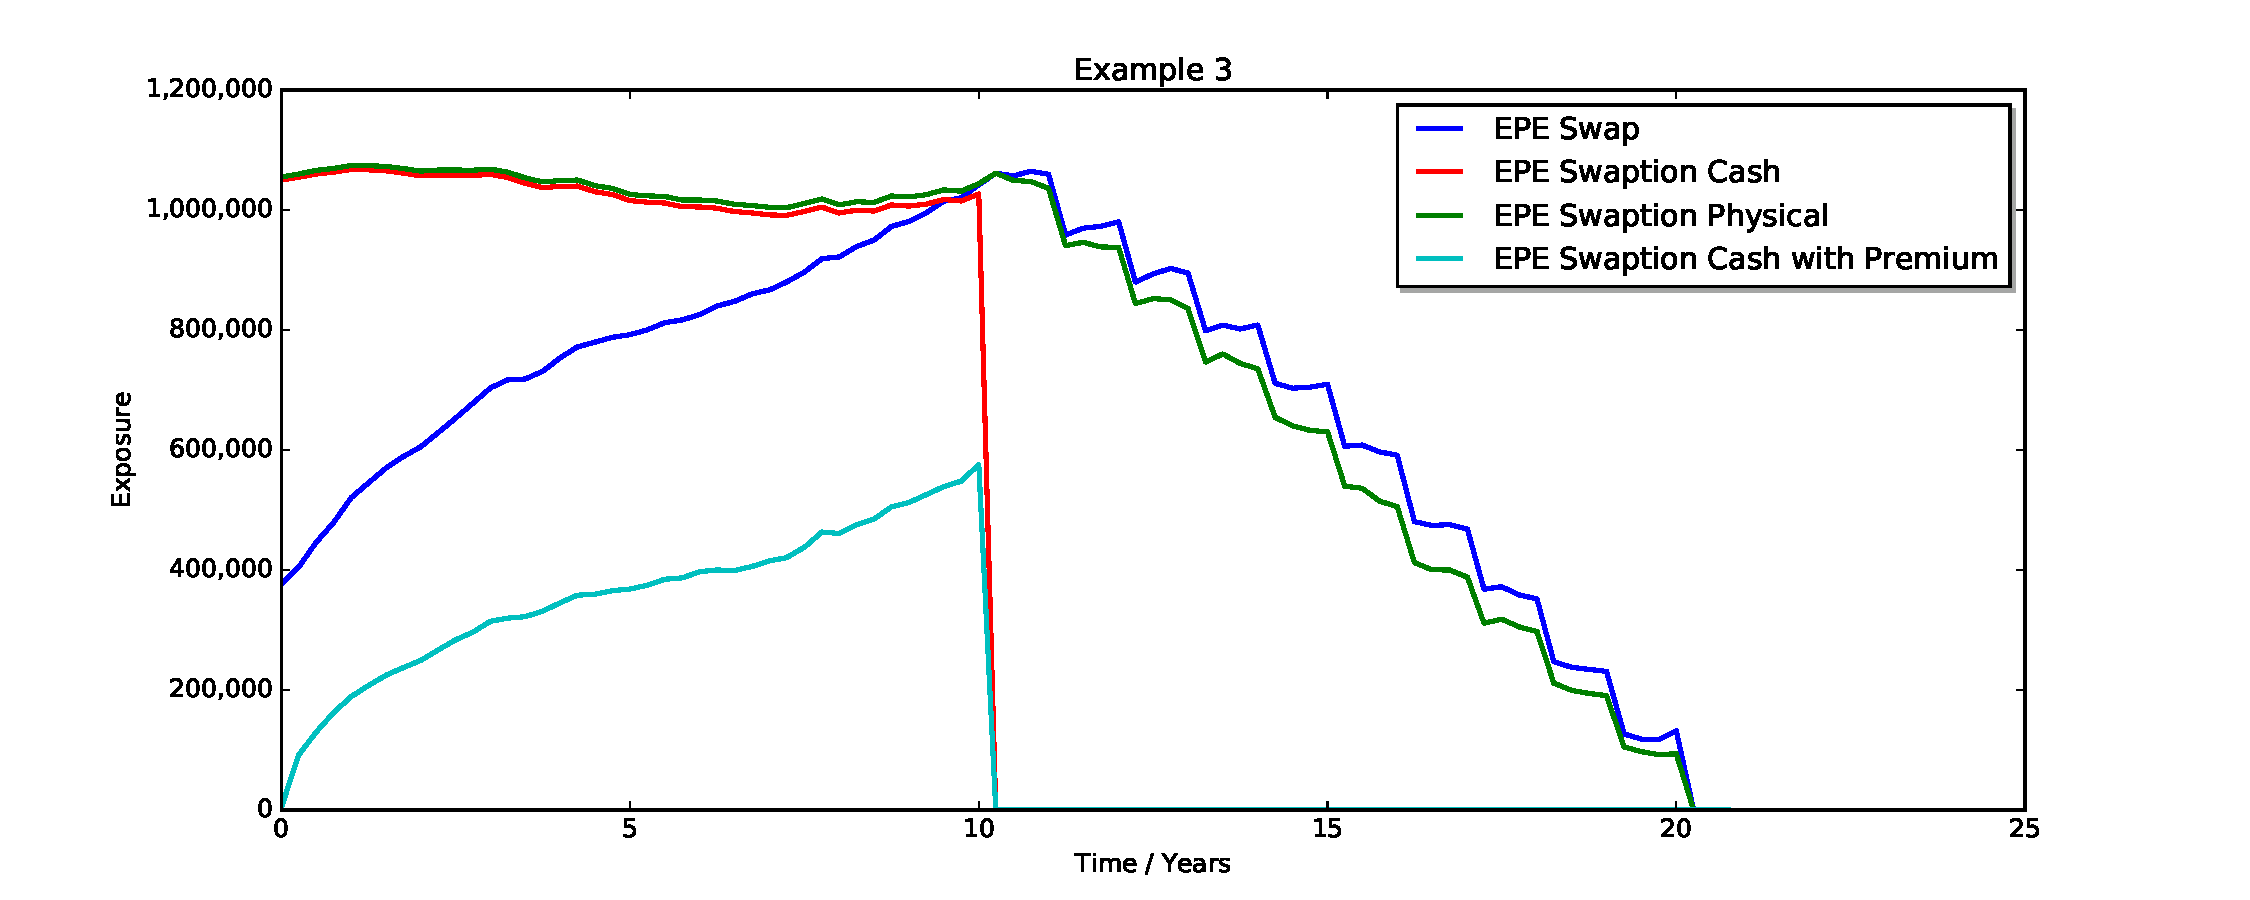
\includegraphics[scale=0.45]{examples/mpl_swaption.pdf}
\end{center}
\caption{European Swaption exposure evolution, expiry in 10 years, final maturity in 20 years, for cash and physical
  delivery. Simulation with 1000 paths and quarterly time steps. }
\label{fig_3}
\end{figure}
The delivery type (cash vs physical) yields significantly different valuations as of today due to the steepness of the
relevant yield curves (EUR). The cash settled Swaption's exposure graph is truncated at the exercise date, whereas the
physically settled Swaption exposure turns into a Swap-like exposure after expiry. For comparison, the example also
provides the exposure evolution of the underlying forward starting Swap which yields a somewhat higher exposure after
the forward start date than the physically settled Swaption. This is due to scenarios with negative Swap NPV at expiry
(hence not exercised) and positive NPVs thereafter. Note the reduced EPE in case of a Swaption with settlement of the option premium on exercise date.

%--------------------------------------------------------
\subsection{Bermudan Swaption Exposure}
%--------------------------------------------------------

This demo case in folder {\tt Examples/Example\_4} shows the exposure evolution of Bermudan rather than European
Swaptions with cash and physical delivery, respectively, see figure \ref{fig_3b}.
\begin{figure}[h!]
\begin{center}
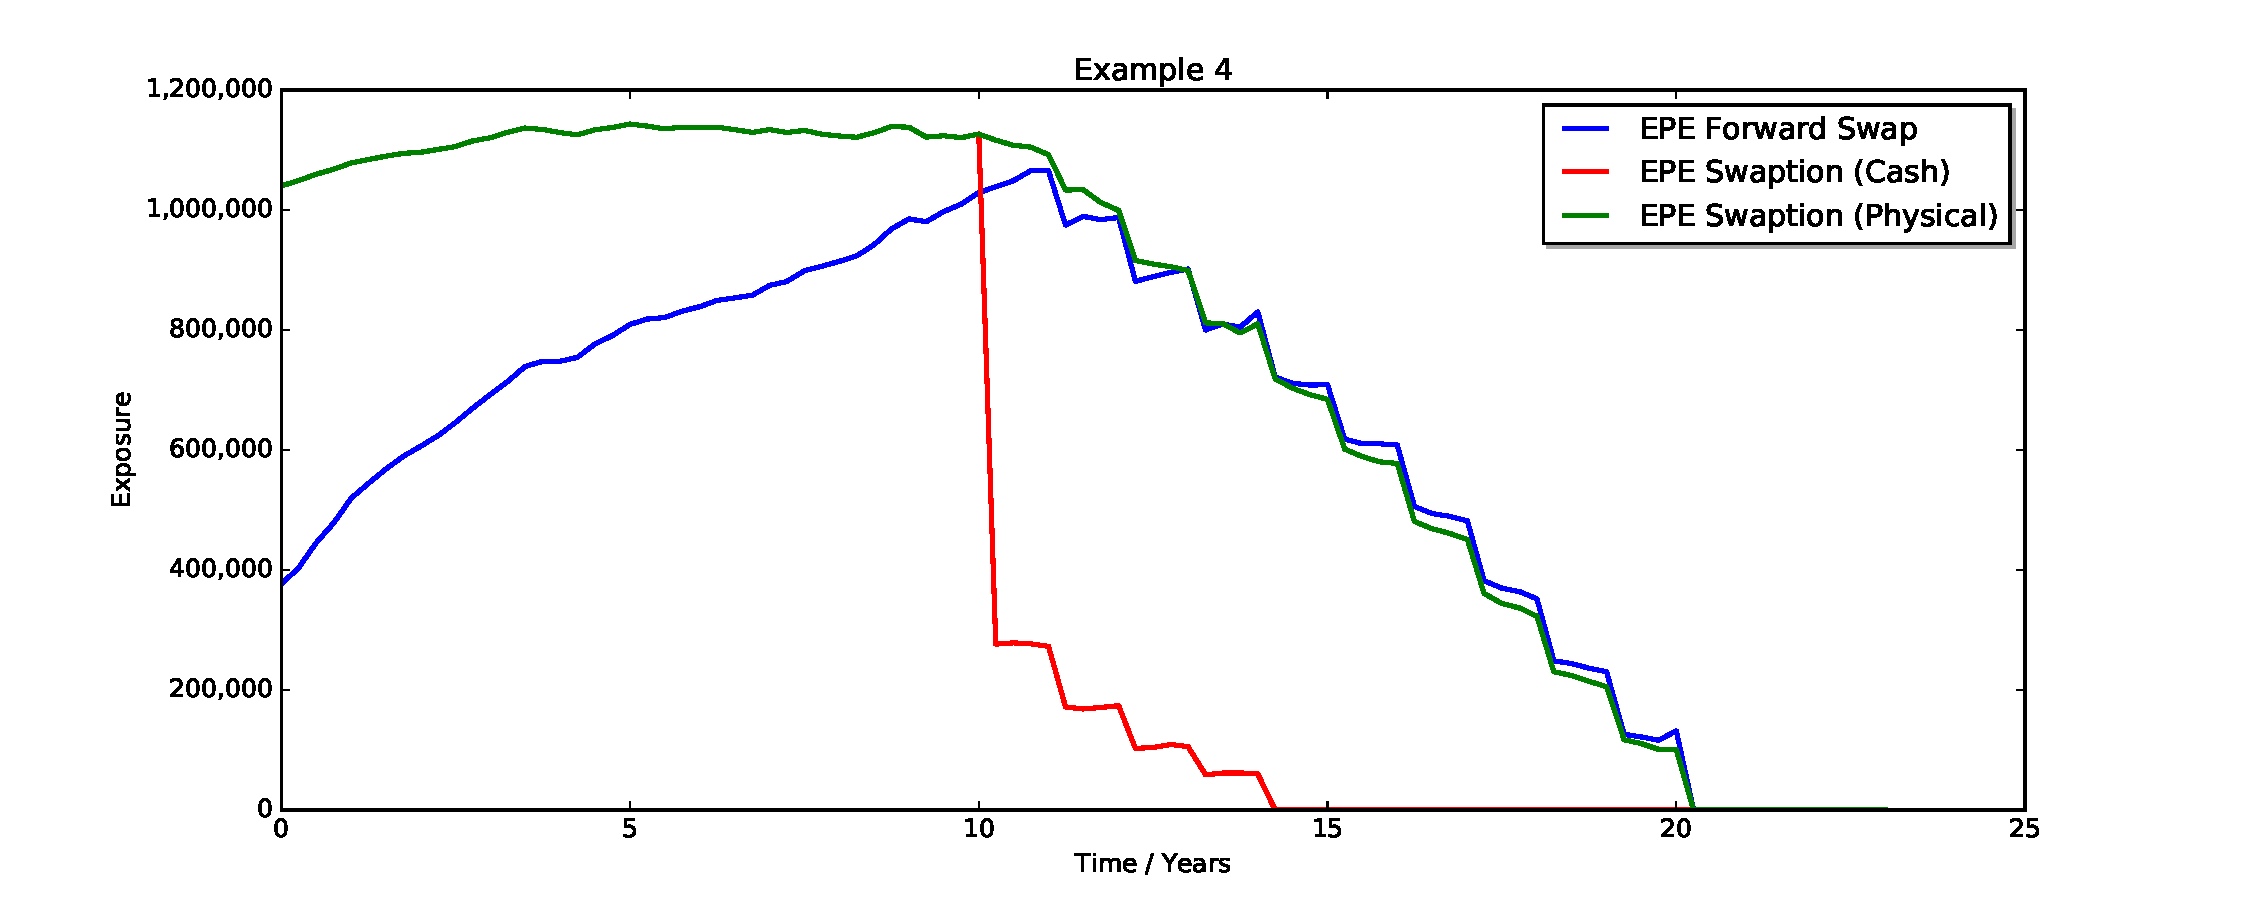
\includegraphics[scale=0.45]{examples/mpl_bermudan_swaption.pdf}
\end{center}
\caption{Bermudan Swaption exposure evolution, 5 annual exercise dates starting in 10 years, final maturity in 20 years,
  for cash and physical delivery. Simulation with 1000 paths and quarterly time steps.}
\label{fig_3b}
\end{figure}
The underlying Swap is the same as in the European Swaption example in section \ref{sec:european_swaption}. Note in
particular the difference between the Bermudan and European Swaption exposures with cash settlement: The Bermudan shows
the typical step-wise decrease due to the series of exercise dates. Also note that we are using the same Bermudan option
pricing engines for both settlement types, in contrast to the European case, so that the Bermudan option cash and
physical exposures are identical up to the first exercise date. When running this example, you will notice the
significant difference in computation time compared to the European case (ballpark 30 minutes here for 2 Swaptions, 1000
samples, 90 time steps). The Bermudan example takes significantly more computation time because we use an LGM grid
engine for pricing under scenarios in this case. In a realistic context one would more likely resort to American Monte
Carlo simulation, feasible in ORE, but not provided in the current release. However, this implementation can be used to
benchmark any faster / more sophisticated approach to Bermudan Swaption exposure simulation.

%--------------------------------------------------------
\subsection{Callable Swap Exposure}
%--------------------------------------------------------

This demo case in folder {\tt Examples/Example\_5} shows the exposure evolution of a European callable Swap, represented
as two trades - the non-callable Swap and a Swaption with physical delivery. We have sold the call option, i.e. the
Swaption is a right for the counterparty to enter into an offsetting Swap which economically terminates all future flows
if exercised. The resulting exposure evolutions for the individual components (Swap, Swaption), as well as the callable
Swap are shown in figure \ref{fig_4}.
\begin{figure}[h!]
\begin{center}
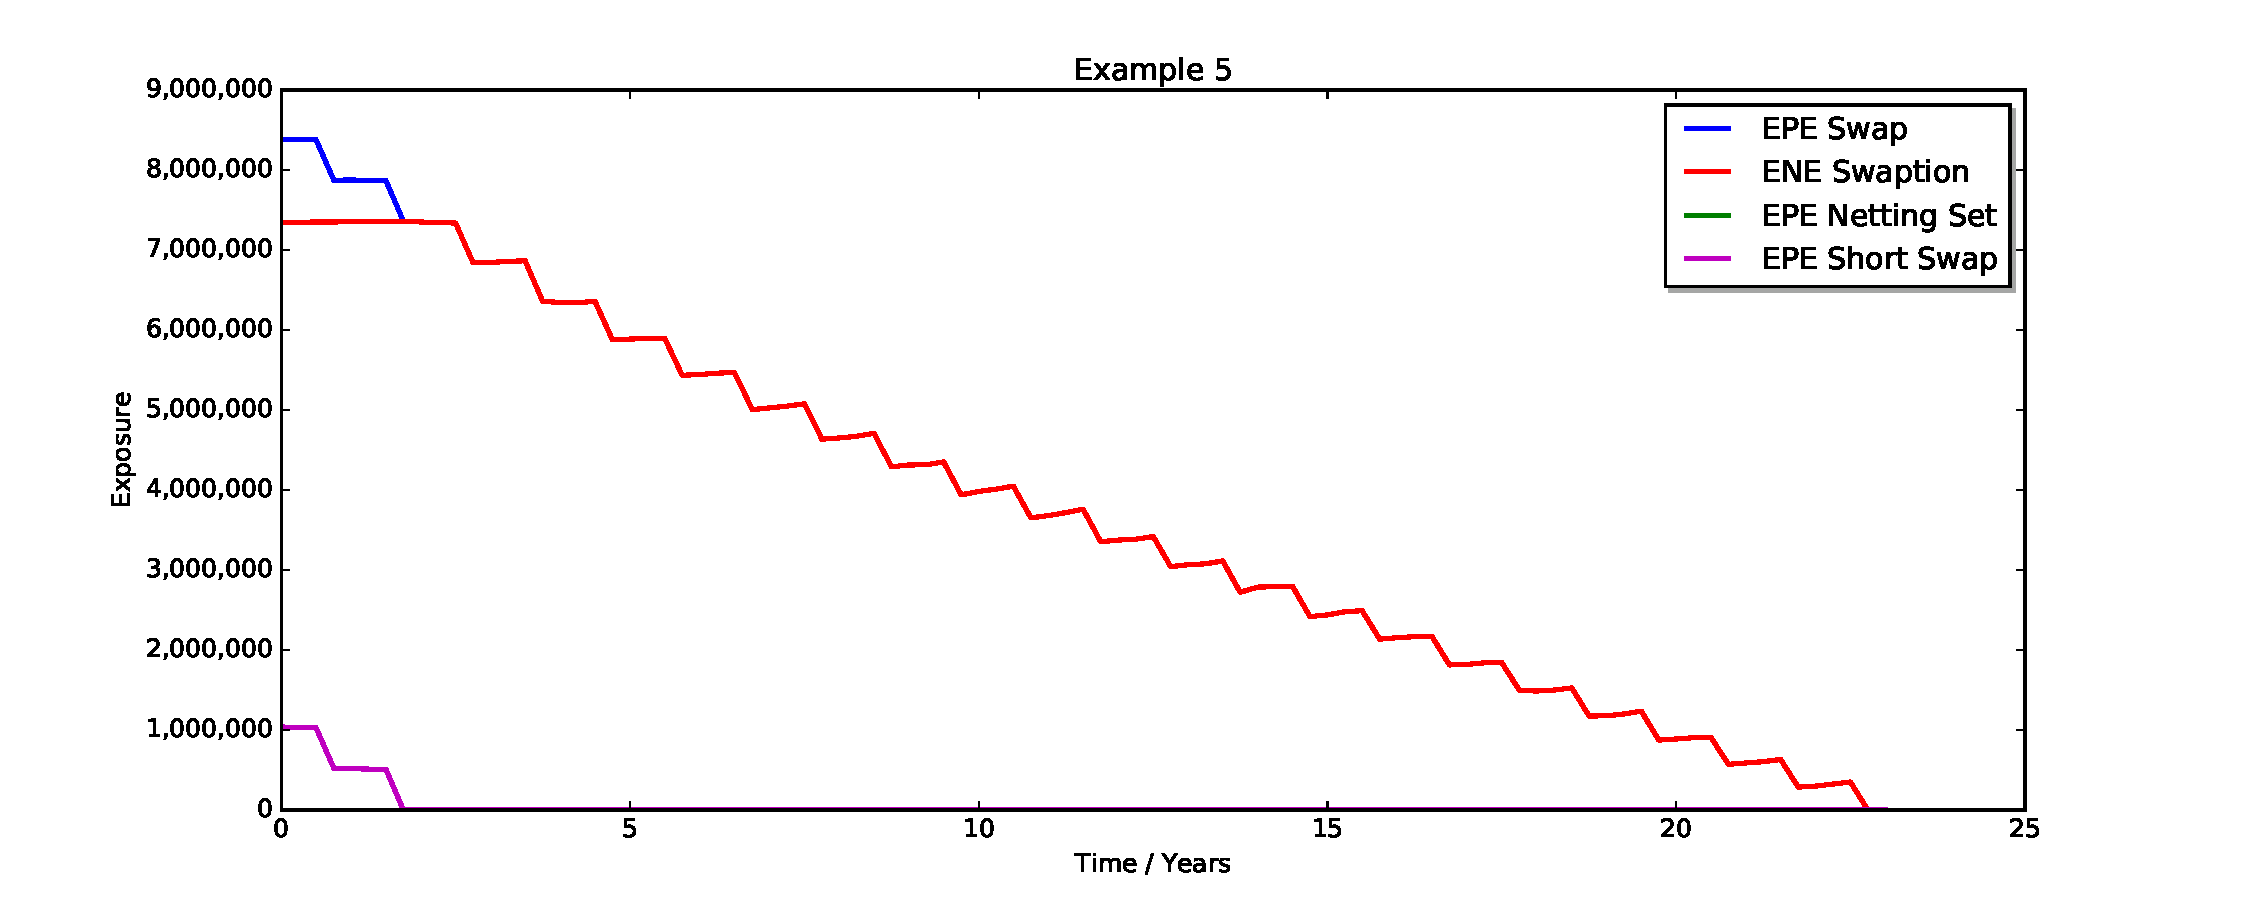
\includegraphics[scale=0.45]{examples/mpl_callable_swap.pdf}
\end{center}
\caption{European callable Swap represented as a package consisiting of non-callable Swap and Swaption. The Swaption has
  physical delivery and offsets all future Swap cash flows if exercised. The exposure evolution of the package is shown
  here as 'EPE Netting Set' (green line). This is covered by the pink line, the exposure evolution of the same Swap but
  with maturity on the exercise date. The graphs match perfectly here, because the example Swap is deep in the money and
  exercise probability is close to one. Simulation with 5000 paths and quarterly time steps.}
\label{fig_4}
\end{figure}
The example is an extreme case where the underlying Swap is deeply in the money (receiving fixed 5\%), and hence the
call exercise probability is close to one. Modify the Swap and Swaption fixed rates closer to the money ($\approx$ 1\%)
to see the deviation between net exposure of the callable Swap and the exposure of a 'short' Swap with maturity on
exercise.

We have added more recently the combined CallableSwap instrument representation, check {\tt portfolio.xml} and compare
the CallableSwap NPV in {\tt npv.csv} to the package NPV of Swap and Swaption.

%--------------------------------------------------------
\subsection{Cap/Floor Exposure}\label{sec:capfloor}
%--------------------------------------------------------

The example in folder {\tt Examples/Example\_6} generates exposure evolutions of several Swaps, caps and floors. The
example shown in figure \ref{fig_capfloor_1} ('portfolio 1') consists of a 20y Swap receiving 3\% fixed and paying
Euribor 6M plus a long 20y Collar
with both cap and floor at 4\% so that the net exposure corresponds to a Swap paying 1\% fixed. \\

\begin{figure}[h!]
\begin{center}
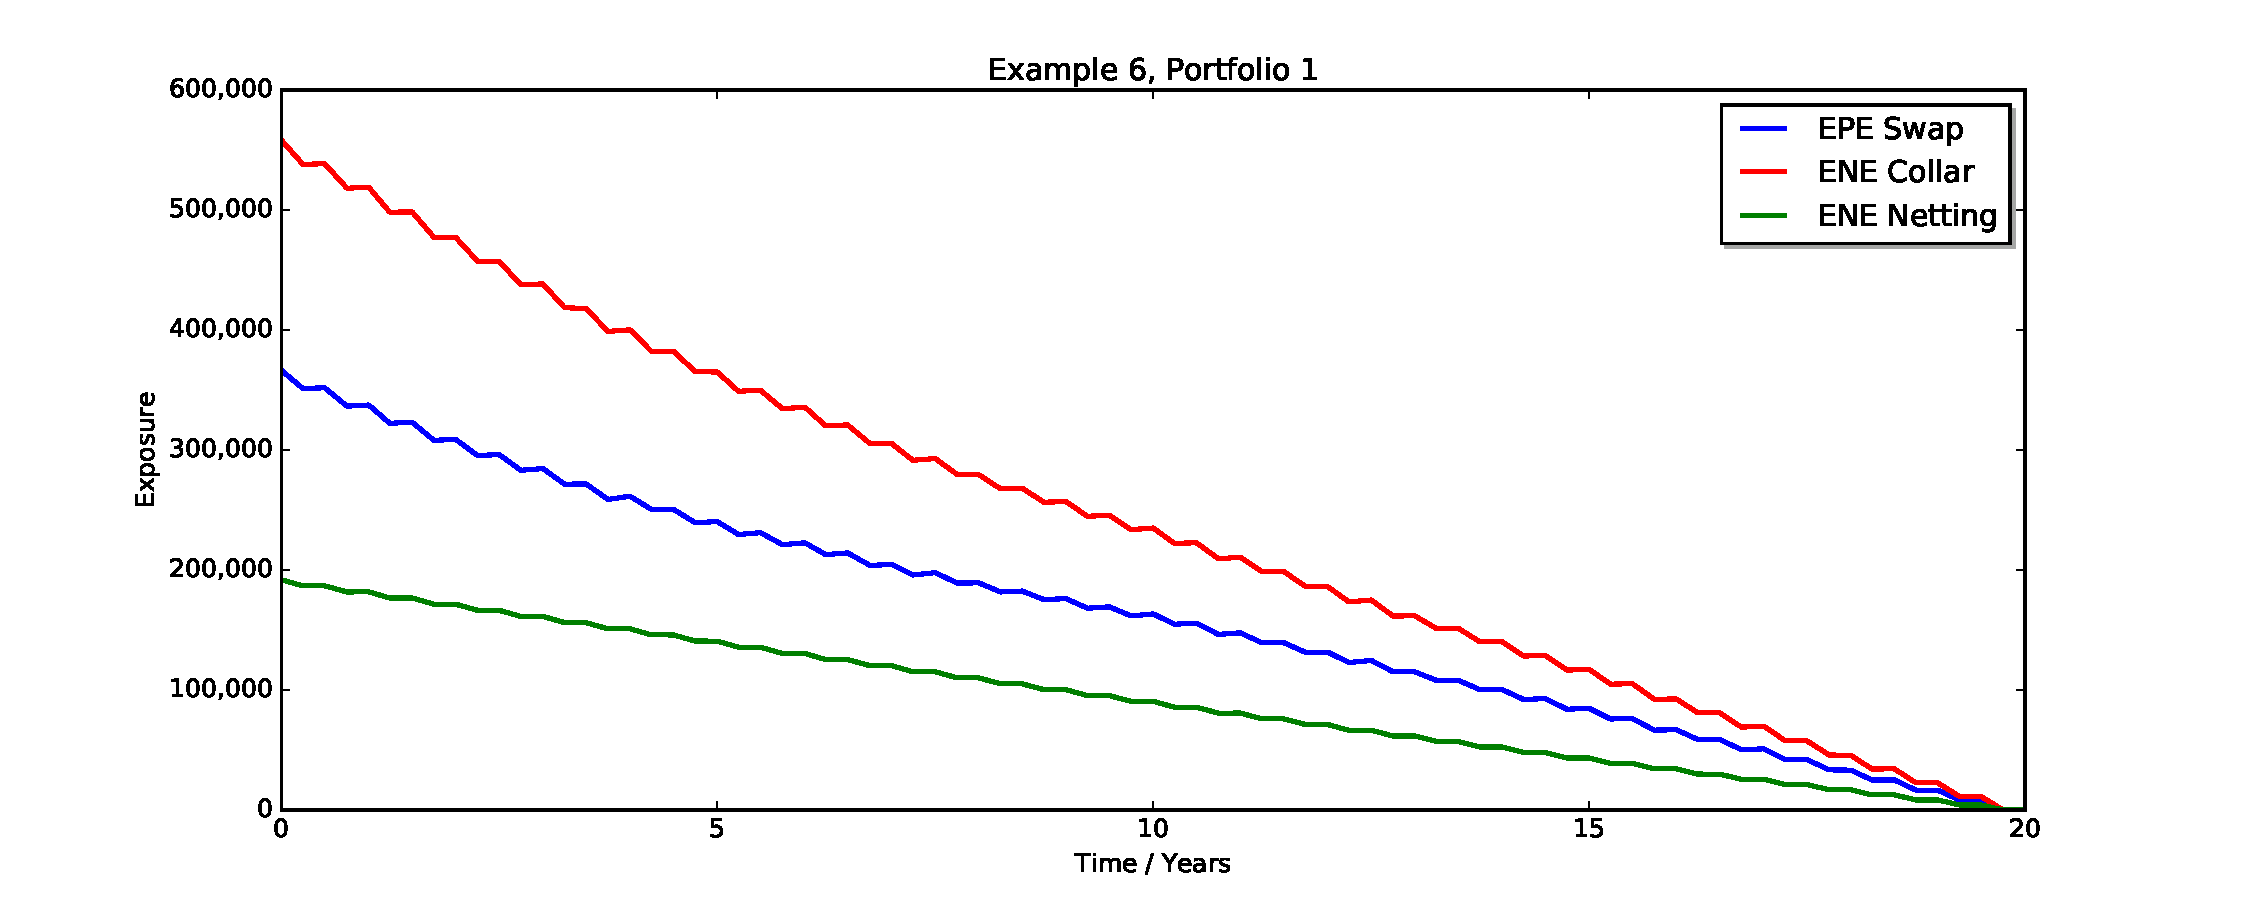
\includegraphics[scale=0.45]{examples/mpl_capfloor_1.pdf}
\end{center}
\caption{Swap+Collar, portfolio 1. The Collar has identical cap and floor rates at 4\% so that it corresponds to a
  fixed leg which reduces the exposure of the Swap, which receives 3\% fixed. Simulation with 1000 paths and quarterly
  time steps.}
\label{fig_capfloor_1}
\end{figure}

The second example in this folder shown in figure \ref{fig_capfloor_2} ('portfolio 2') consists of a short Cap, long
Floor and a long Collar that exactly offsets the netted Cap and Floor.

\begin{figure}[h!]
\begin{center}
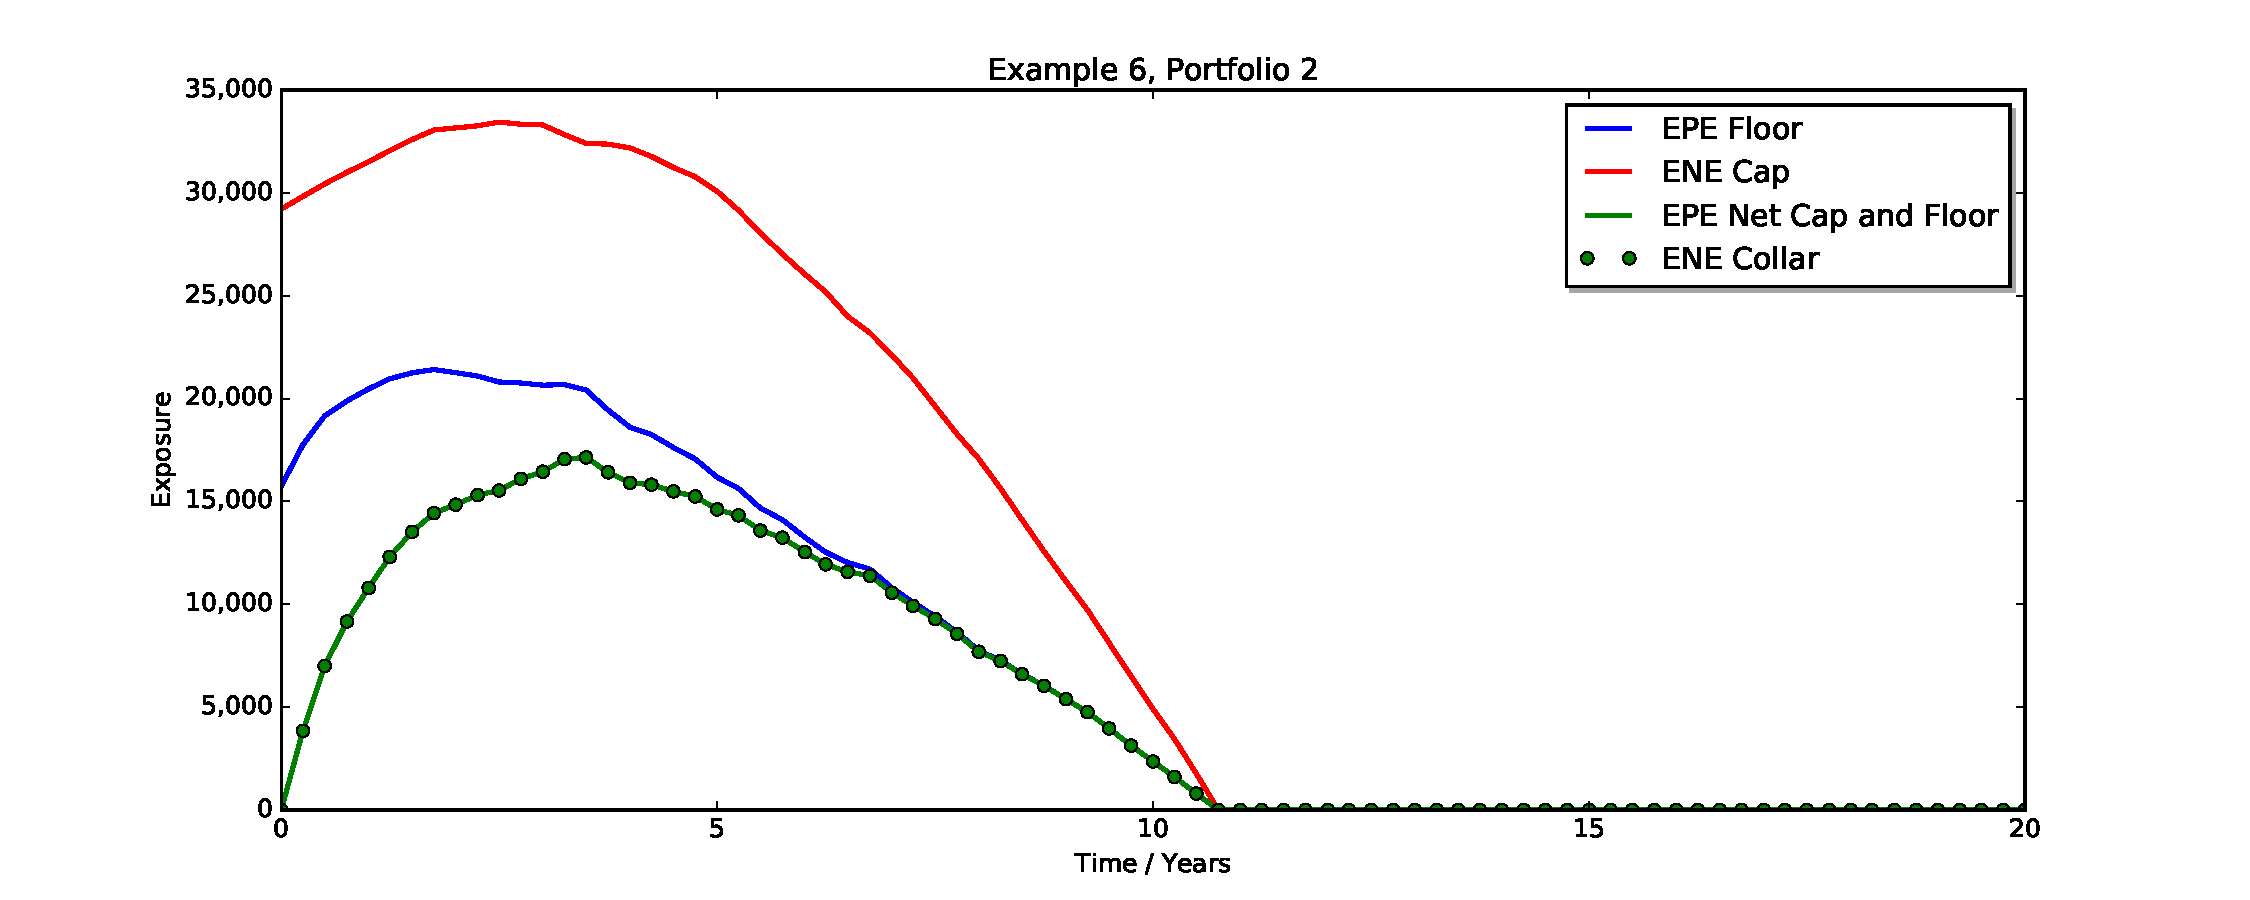
\includegraphics[scale=0.45]{examples/mpl_capfloor_2.pdf}
\end{center}
\caption{Short Cap and long Floor vs long Collar, portfolio 2. Simulation with 1000 paths and quarterly time steps.}
\label{fig_capfloor_2}
\end{figure}

Further three test portfolios are provided as part of this example. Run the example and inspect the respective output
directories {\tt Examples/Example\_6/Output/portfolio\_\#}. Note that these directories have to be present/created
before running the batch with {\tt python run.py}.

%--------------------------------------------------------
\subsection{FX Forward and FX Option Exposure}\label{sec:fxfwd}
%--------------------------------------------------------

The example in folder {\tt Examples/Example\_7} generates the exposure evolution for a EUR / USD FX Forward transaction
with value date in 10Y. This is a particularly simple show case because of the single cash flow in 10Y. On the other
hand it checks the cross currency model implementation by means of comparison to analytic limits - EPE and ENE at the
trade's value date must match corresponding Vanilla FX Option prices, as shown in figure \ref{fig_5}.
\begin{figure}[h]
\begin{center}
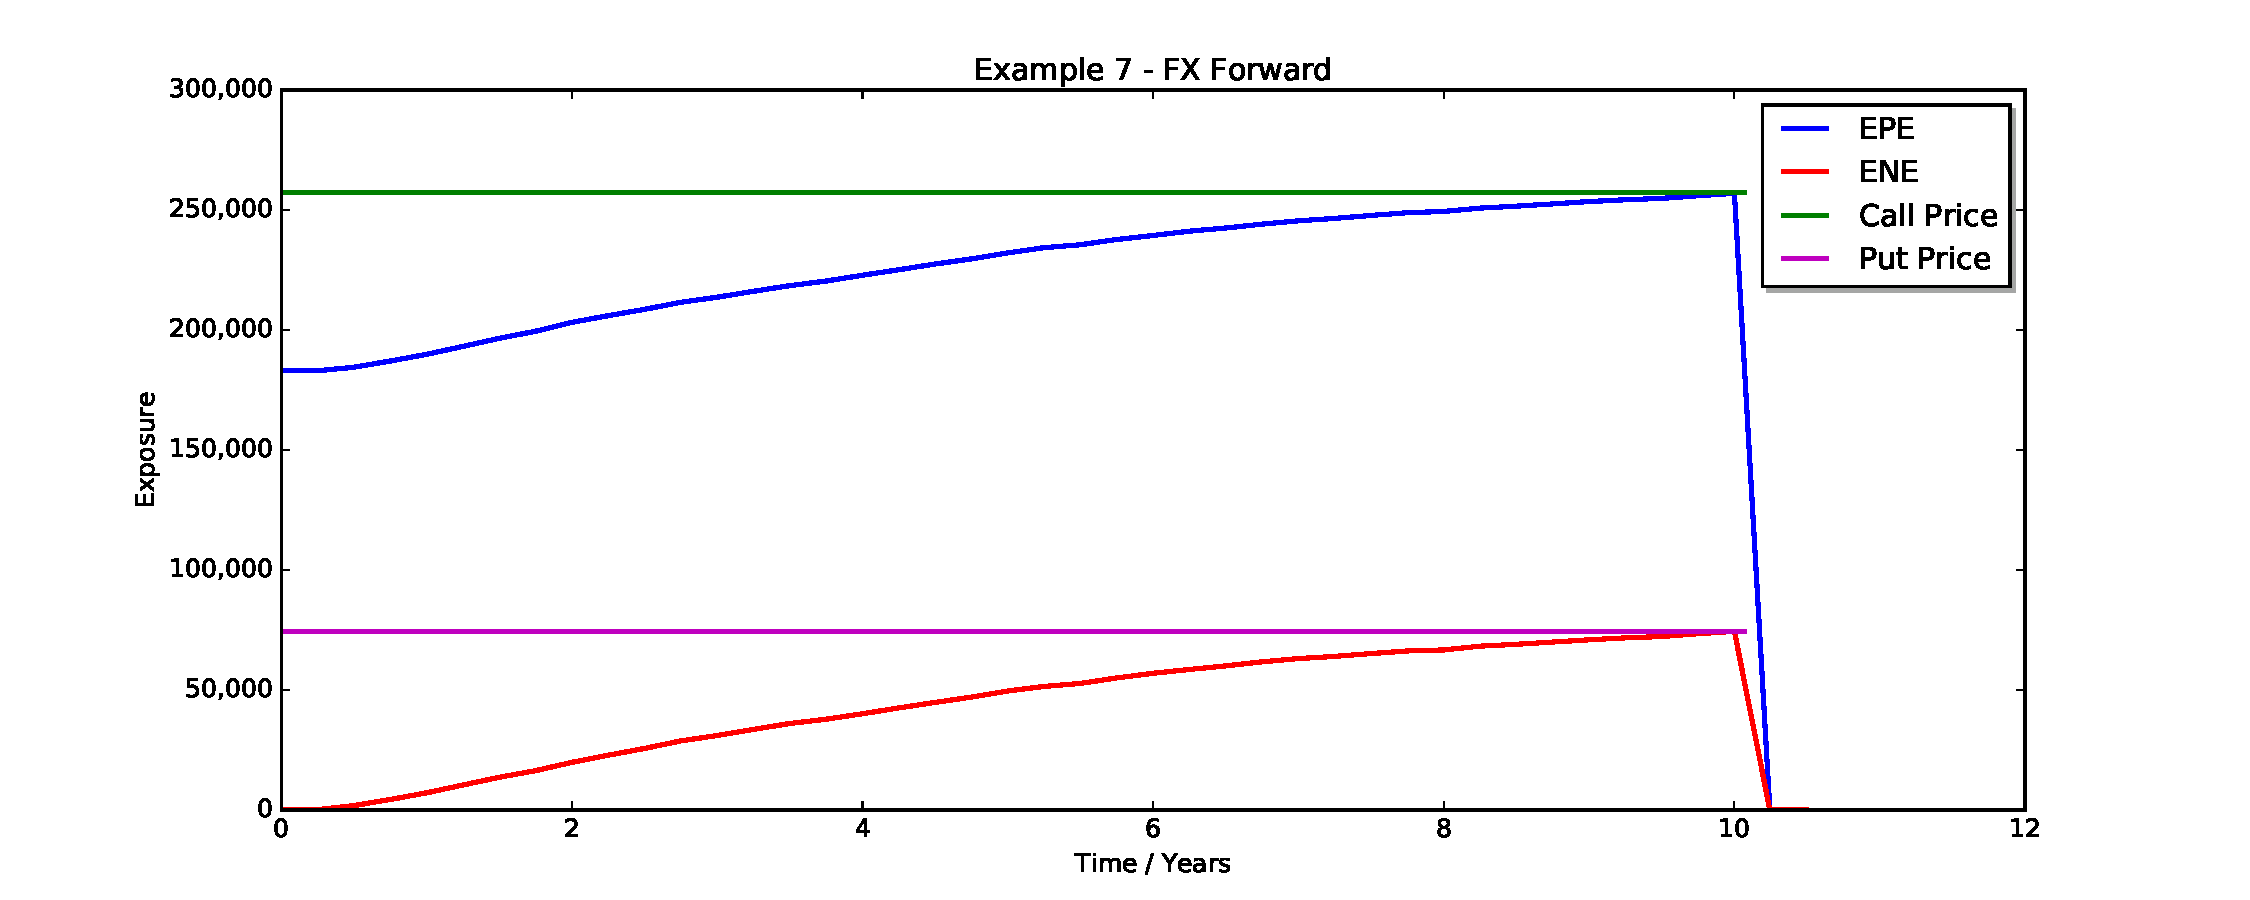
\includegraphics[scale=0.45]{examples/mpl_fxforward.pdf}
\end{center}
\caption{EUR/USD FX Forward expected exposure in a realistic market environment as of 26/02/2016 from both parties'
  perspectives. Value date is obviously in 10Y. The flat lines are FX Option prices which coincide with EPE and ENE,
  respectively, on the value date. Simulation with 5000 paths and quarterly time steps.}
\label{fig_5}
\end{figure}

%--------------------------------------------------------
\subsection*{FX Option Exposure}\label{sec:fxoption}
%--------------------------------------------------------

This example (in folder {\tt Examples/Example\_7}, as the FX Forward example) illustrates the exposure evolution for an
FX Option, see figure \ref{fig_7}.
\begin{figure}[h!]
\begin{center}
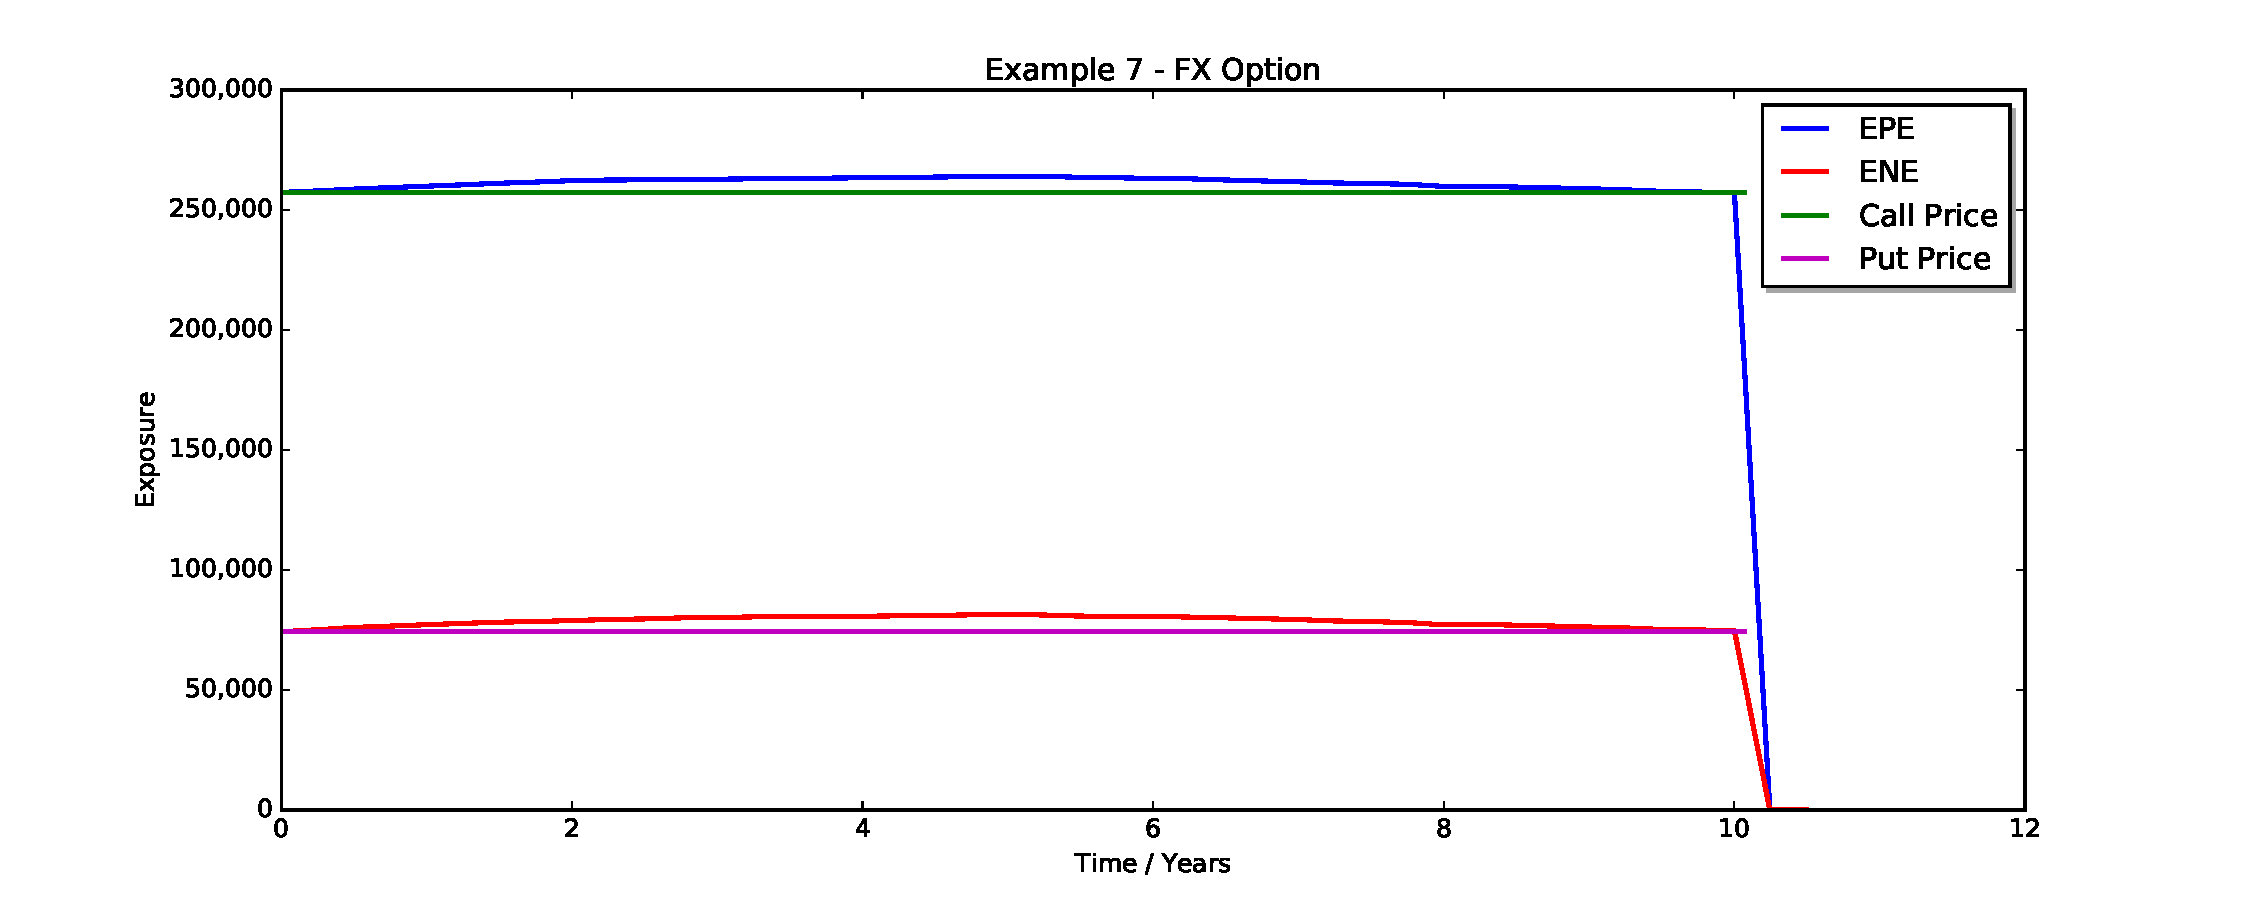
\includegraphics[scale=0.45]{examples/mpl_fxoption.pdf}
\end{center}
\caption{EUR/USD FX Call and Put Option exposure evolution, same underlying and market data as in section
  \ref{sec:fxfwd}, compared to the call and put option price as of today (flat line). Simulation with 5000 paths and
  quarterly time steps.}
\label{fig_7}
\end{figure}
Recall that the FX Option value $NPV(t)$ as of time $0 \leq t \leq T$ satisfies
\begin{align*}
\frac{NPV(t)}{N(t)} &= \mbox{Nominal}\times\E_t\left[\frac{(X(T) - K)^+}{N(T)}\right]\\
NPV(0) &= \E\left[\frac{NPV(t)}{N(t)}\right] = \E\left[\frac{NPV^+(t)}{N(t)} \right]= \EPE(t) 
\end{align*}
where $N(t)$ denotes the numeraire asset.
One would therefore expect a flat exposure evolution up to option expiry. The deviation from this in ORE's simulation is
due to the pricing approach chosen here under scenarios. A Black FX option pricer is used with deterministic Black
volatility derived from today's volatility structure (pushed or rolled forward, see section \ref{sec:sim_market}). The
deviation can be removed by extending the volatility modelling, e.g. implying model consistent Black volatilities in
each simulation step on each path.  
%\todo[inline]{Add exposure evolution graph with 'simulated' FX vol}

%--------------------------------------------------------
\subsection{Cross Currency Swap Exposure, without FX Reset}
%--------------------------------------------------------

The case in {\tt Examples/Example\_8} is a vanilla cross currency Swap. It shows the typical blend of an Interest Rate
Swap's saw tooth exposure evolution with an FX Forward's exposure which increases monotonically to final maturity, see
figure \ref{fig_6}.
\begin{figure}[h!]
\begin{center}
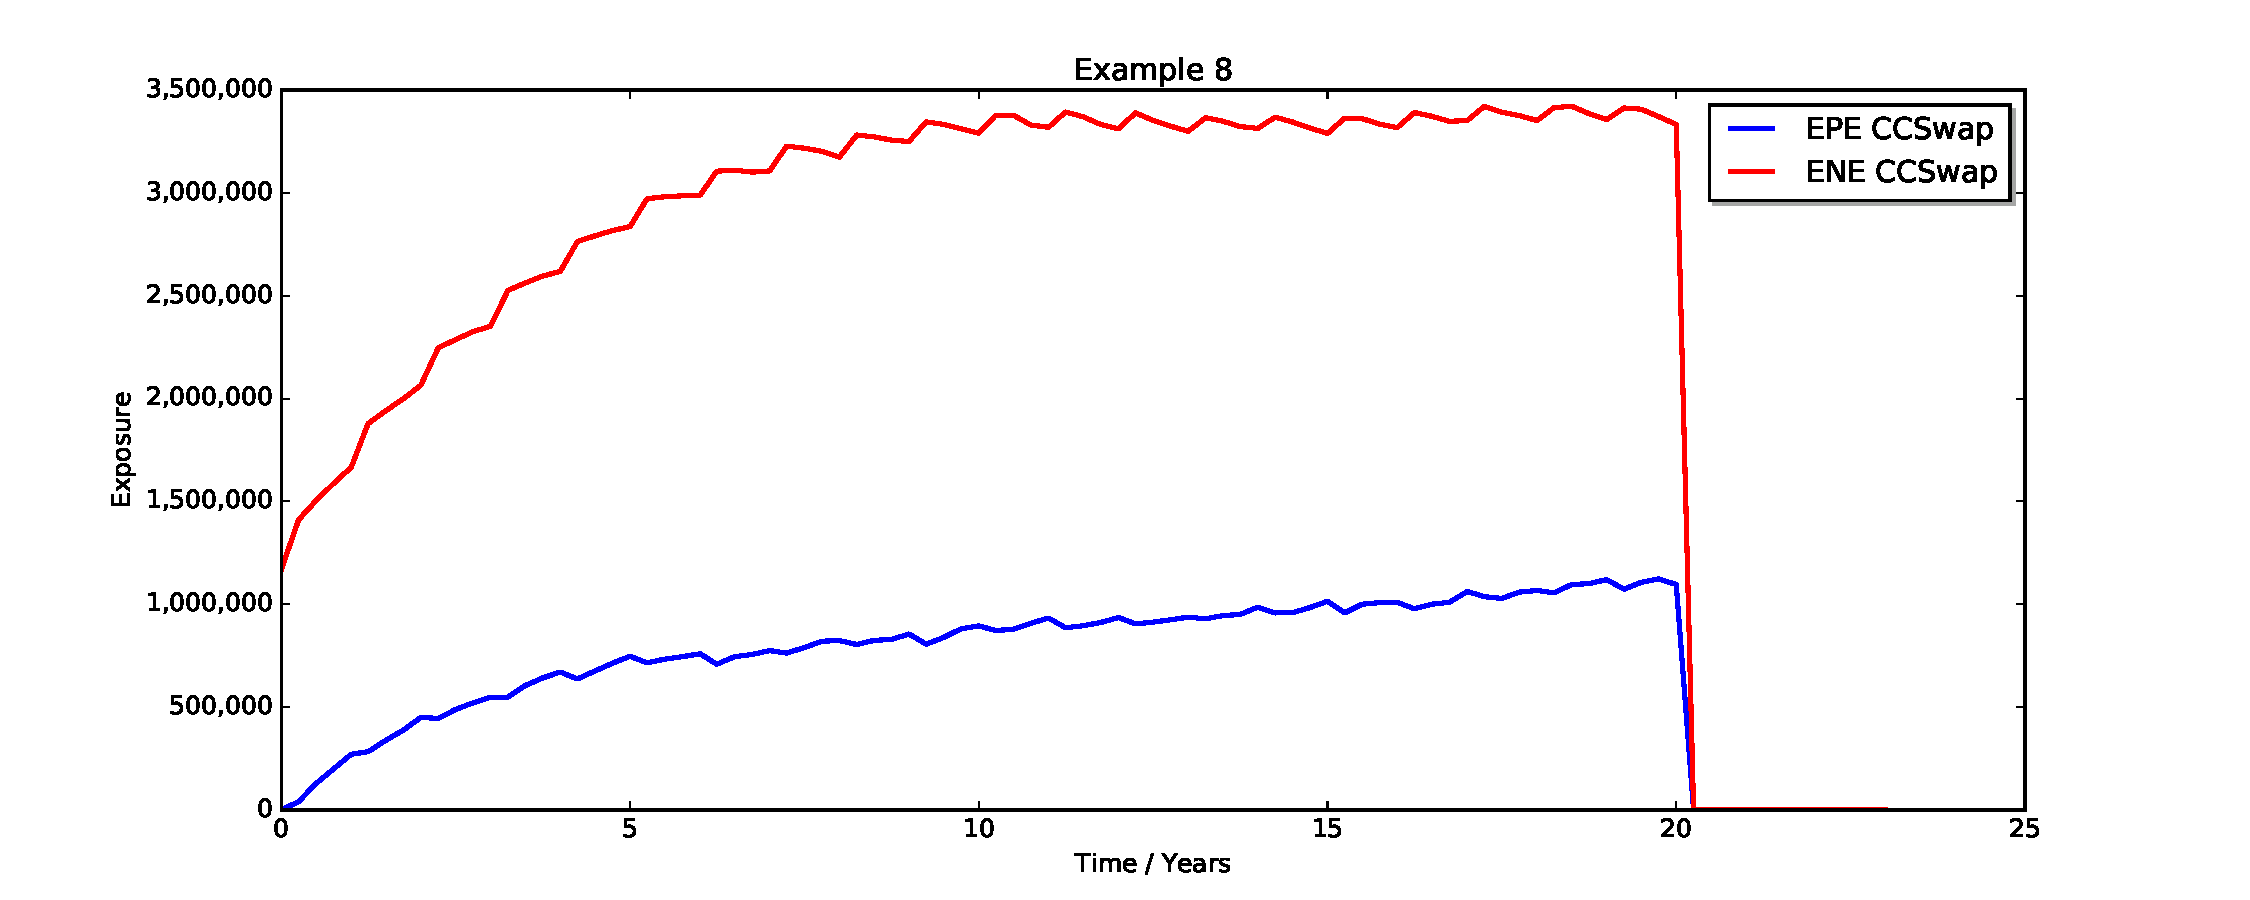
\includegraphics[scale=0.45]{examples/mpl_ccswap.pdf}
\end{center}
\caption{Cross Currency Swap exposure evolution without mark-to-market notional reset. Simulation with 1000 paths and
  quarterly time steps.}
\label{fig_6}
\end{figure}

{\tt Examples/Example\_8} also demonstrates the ``serialization'' of the calibrated simulation model, see {\tt Output/calibration.xml} and {\tt Output/calibration.csv}, as well as the brief documentation of the {\tt calibration} analytic in section \ref{sec:analytics}.

%--------------------------------------------------------
\subsection{Cross Currency Swap Exposure, with FX Reset}
%--------------------------------------------------------

The effect of the FX resetting feature, common in Cross Currency Swaps nowadays, is shown in {\tt Examples/Example\_9}.
The example shows the exposure evolution of a EUR/USD cross currency basis Swap with FX reset at each interest period
start, see figure \ref{fig_6b}. As expected, the notional reset causes an exposure collapse at each period start when
the EUR leg's notional is reset to match the USD notional.
\begin{figure}[h!]
\begin{center}
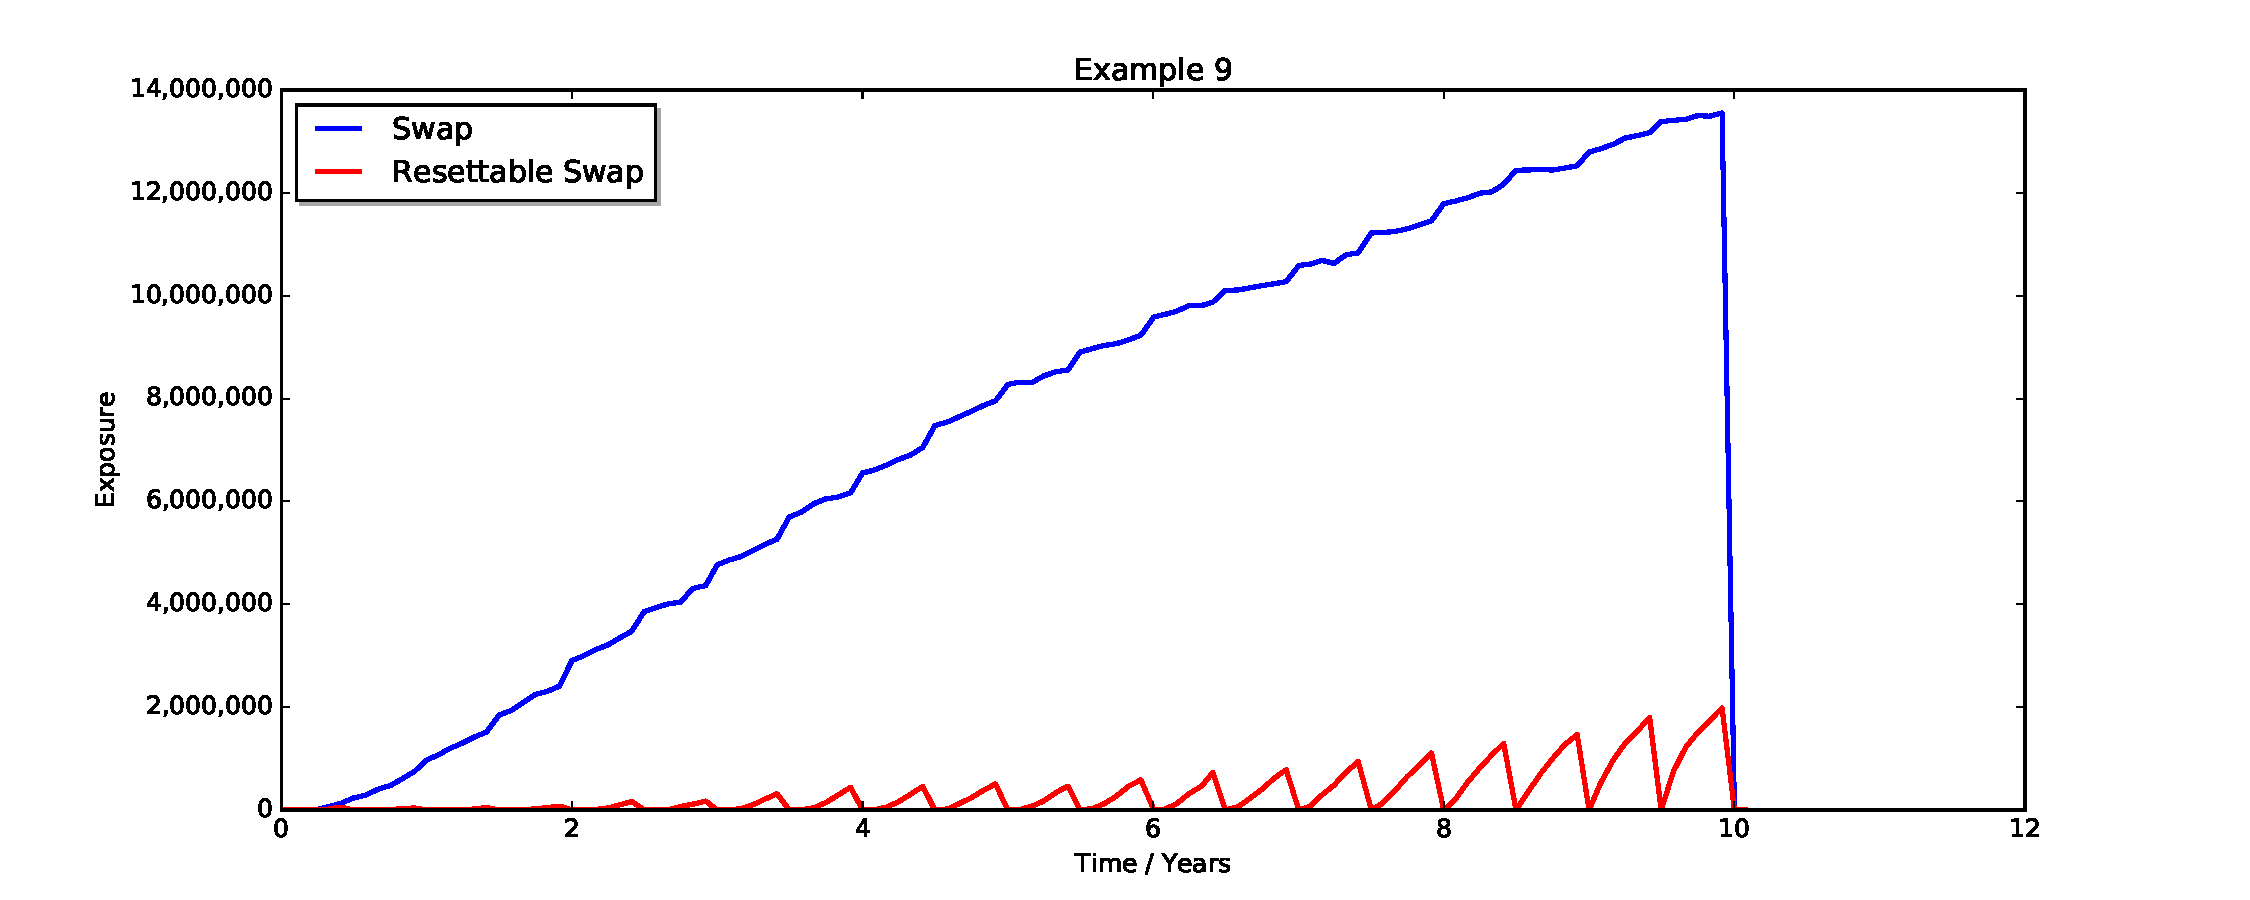
\includegraphics[scale=0.45]{examples/mpl_xccy_reset.pdf}
\end{center}
\caption{Cross Currency Basis Swap exposure evolution with and without mark-to-market notional reset. Simulation with
  1000 paths and quarterly time steps.}
\label{fig_6b}
\end{figure}
  
%--------------------------------------------------------
\subsection{Netting Set, Collateral, XVAs, XVA Allocation}
%--------------------------------------------------------

In this example (see folder {\tt Examples/Example\_10}) we showcase a small netting set consisting of three Swaps in
different currencies, with different collateral choices
\begin{itemize}
\item no collateral - figure \ref{fig_8},
\item collateral with threshold (THR) 1m EUR, minimum transfer amount (MTA) 100k EUR, margin period of risk (MPOR) 2
  weeks - figure \ref{fig_9}
\item collateral with zero THR and MTA, and MPOR 2w - figure \ref{fig_10}
\end{itemize}
The exposure graphs with collateral and positive margin period of risk show typical spikes. What is causing these? As
sketched in \cite{methods}, ORE uses a {\em classical collateral model} that applies collateral
amounts to offset exposure with a time delay that corresponds to the margin period of risk. The spikes are then caused
by instrument cash flows falling between exposure measurement dates $d_1$ and $d_2$ (an MPOR apart), so that a
collateral delivery amount determined at $d_1$ but settled at $d_2$ differs significantly from the closeout amount at
$d_2$ causing a significant residual exposure for a short period of time. See for example \cite{Andersen2016} for a
recent detailed discussion of collateral modelling. The approach currently implemented in ORE corresponds to {\em
  Classical+} in \cite{Andersen2016}, the more conservative approach of the classical methods. The less conservative
alternative, {\em Classical-}, would assume that both parties stop paying trade flows at the beginning of the MPOR, so
that the P\&L over the MPOR does not contain the cash flow effect, and exposure spikes are avoided. Note that the size
and position of the largest spike in figure \ref{fig_9} is consistent with a cash flow of the 40 million GBP Swap in the
example's portfolio that rolls over the 3rd of March and has a cash flow on 3 March 2020, a bit more than four years
from the evaluation date.
  
\begin{figure}[h!]
\begin{center}
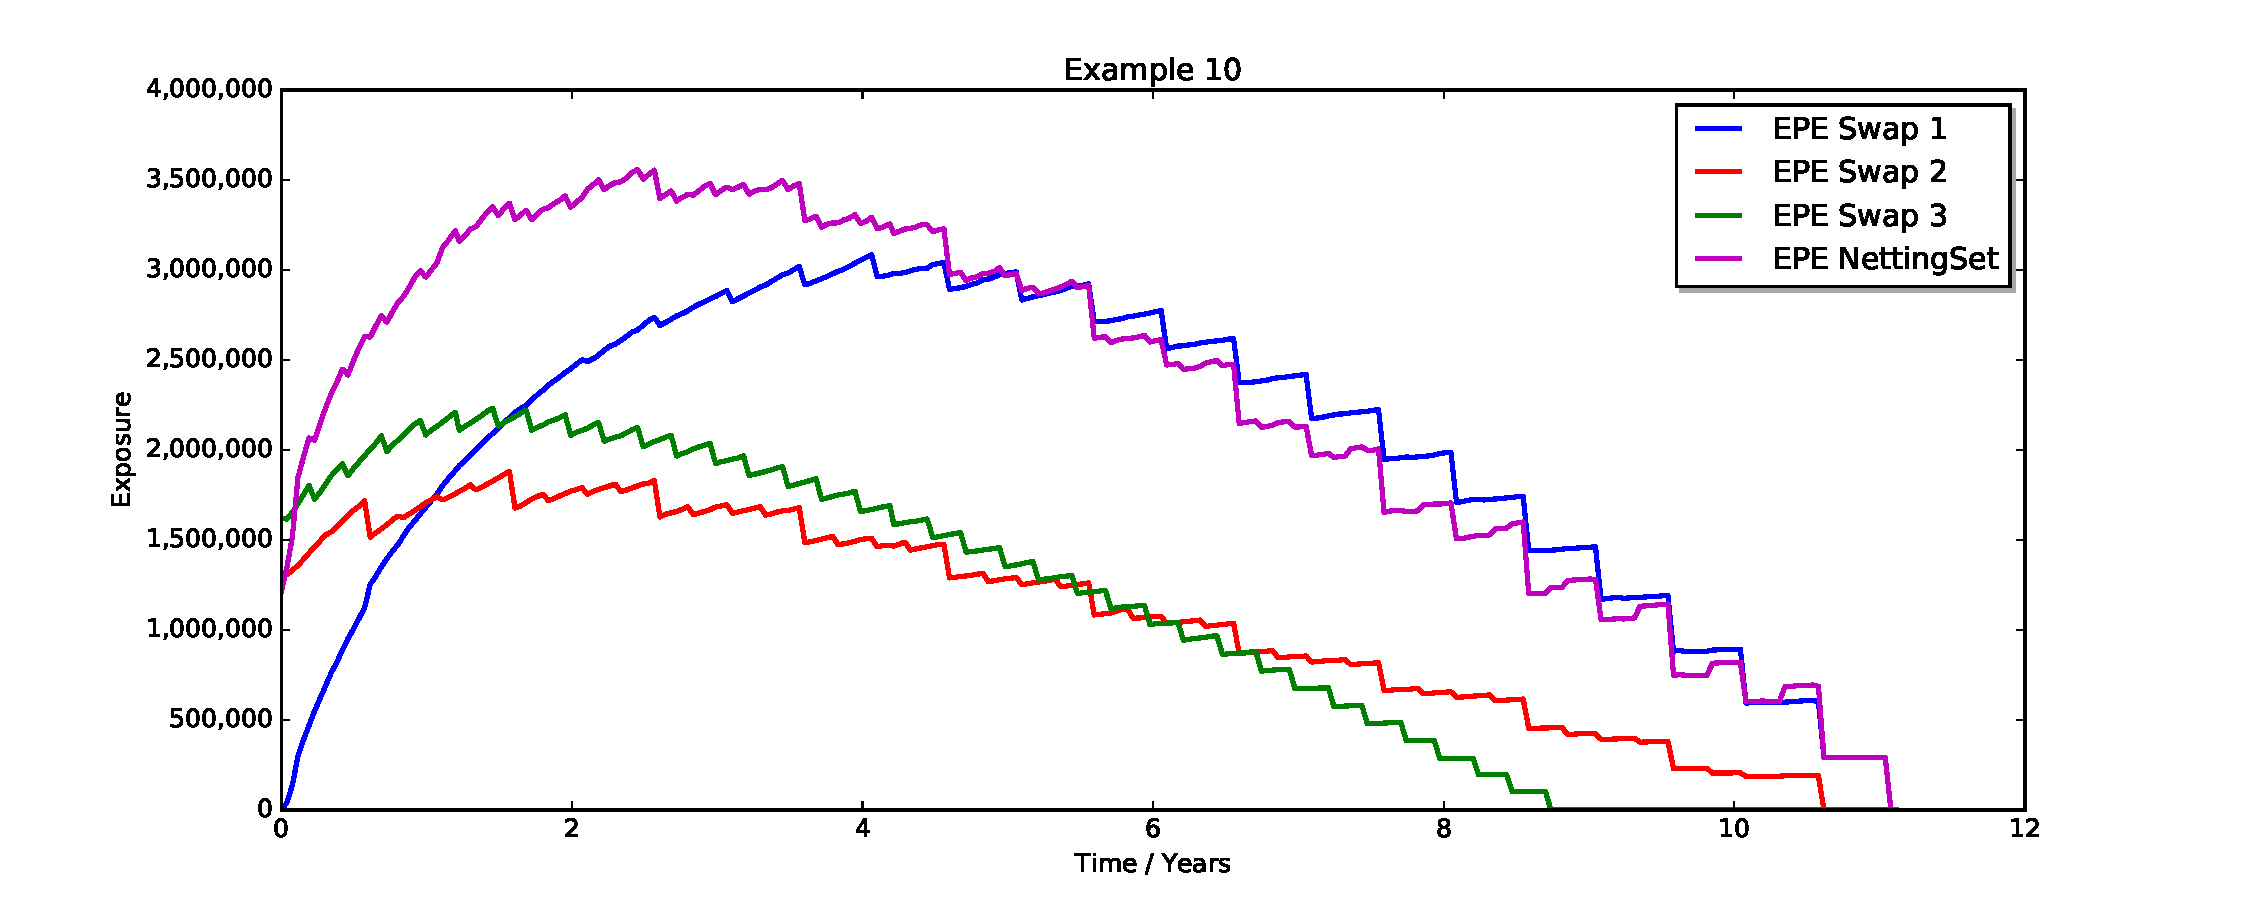
\includegraphics[scale=0.45]{examples/mpl_nocollateral_epe.pdf}
\end{center}
\caption{Three Swaps netting set, no collateral. Simulation with 5000 paths and bi-weekly time steps.}
\label{fig_8}
\end{figure}

\begin{figure}[htb]
\begin{center}
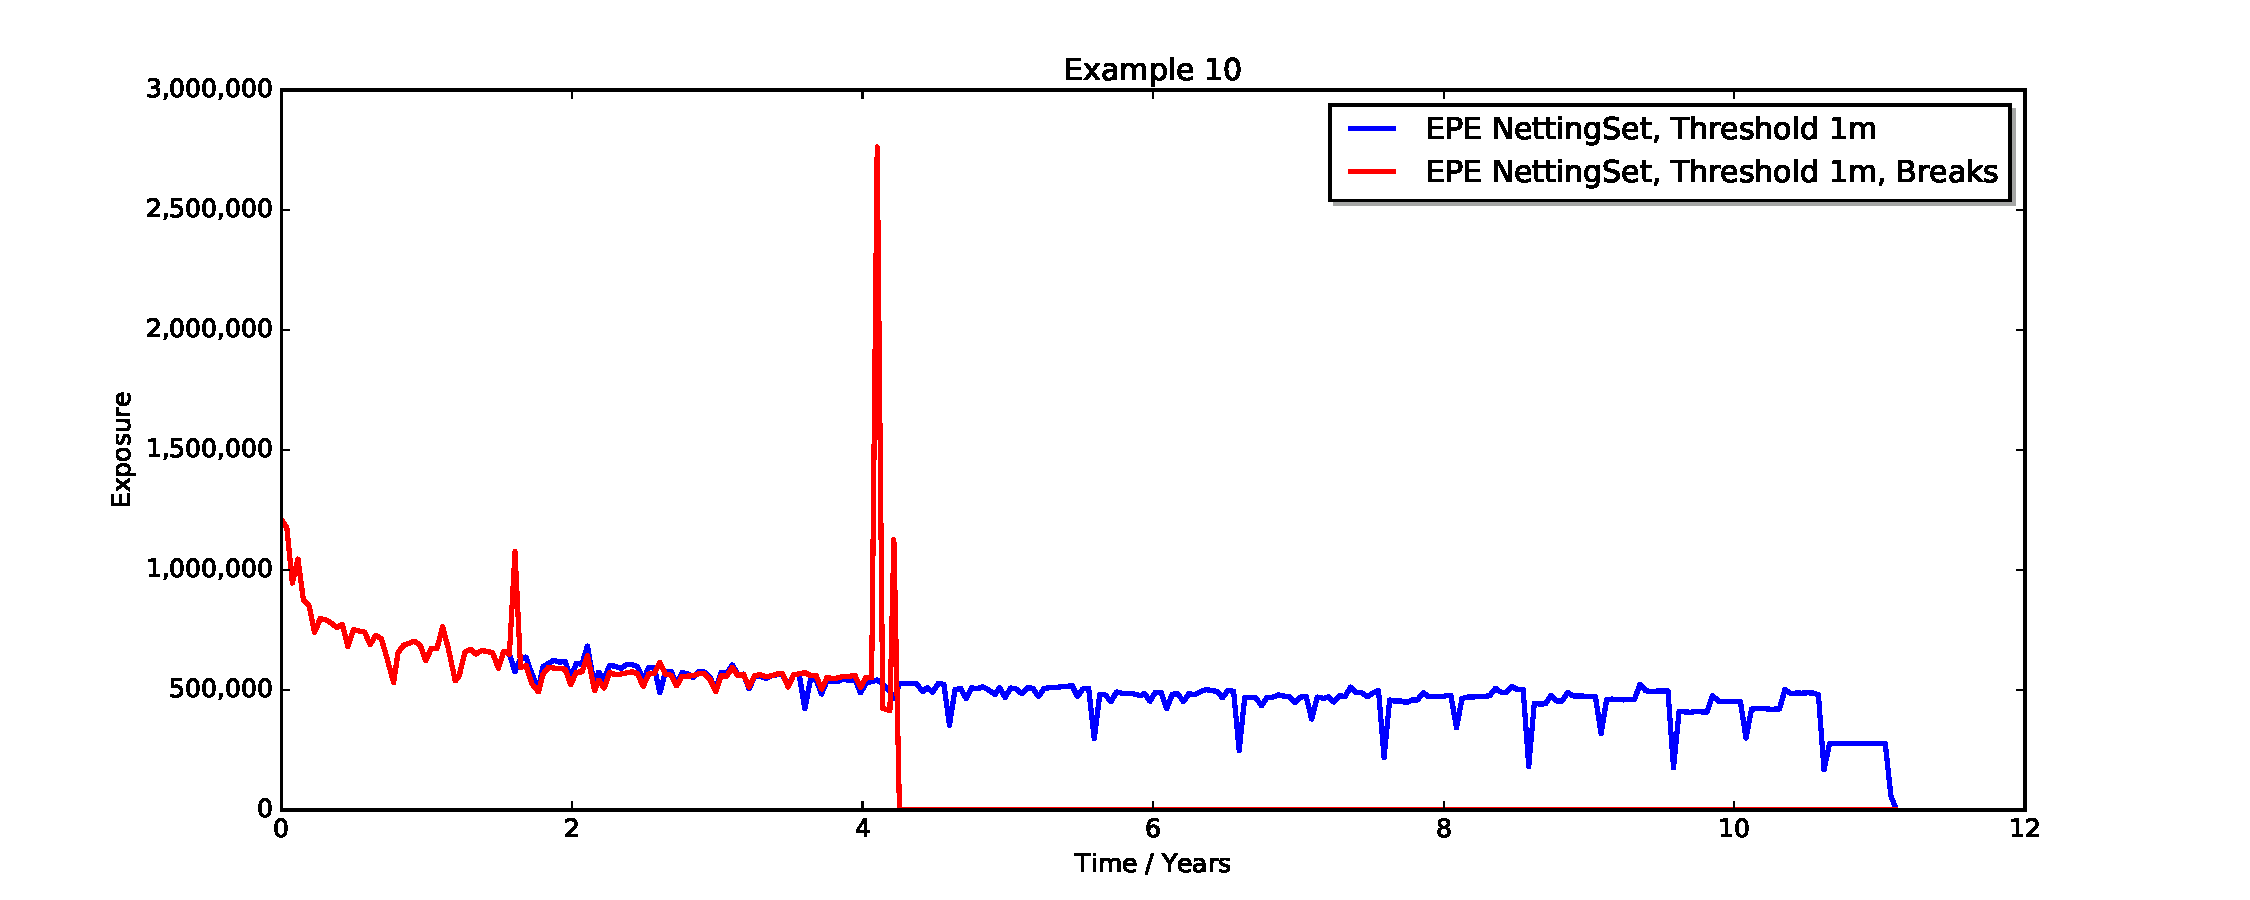
\includegraphics[scale=0.45]{examples/mpl_threshold_break_epe.pdf}
\end{center}
\caption{Three Swaps netting set, THR=1m EUR, MTA=100k EUR, MPOR=2w. The red evolution assumes that the each trade is
  terminated at the next break date. The blue evolution ignores break dates. Simulation with 5000 paths and bi-weekly
  time steps.}
\label{fig_9}
\end{figure}

%\begin{figure}[h]
%\begin{center}
%\includegraphics[scale=1.0]{example_mta_epe.pdf}
%\end{center}
%\caption{Three swaps, threshold = 0, mta > 0.}
%\label{fig_7}
%\end{figure}

\begin{figure}[h!]
\begin{center}
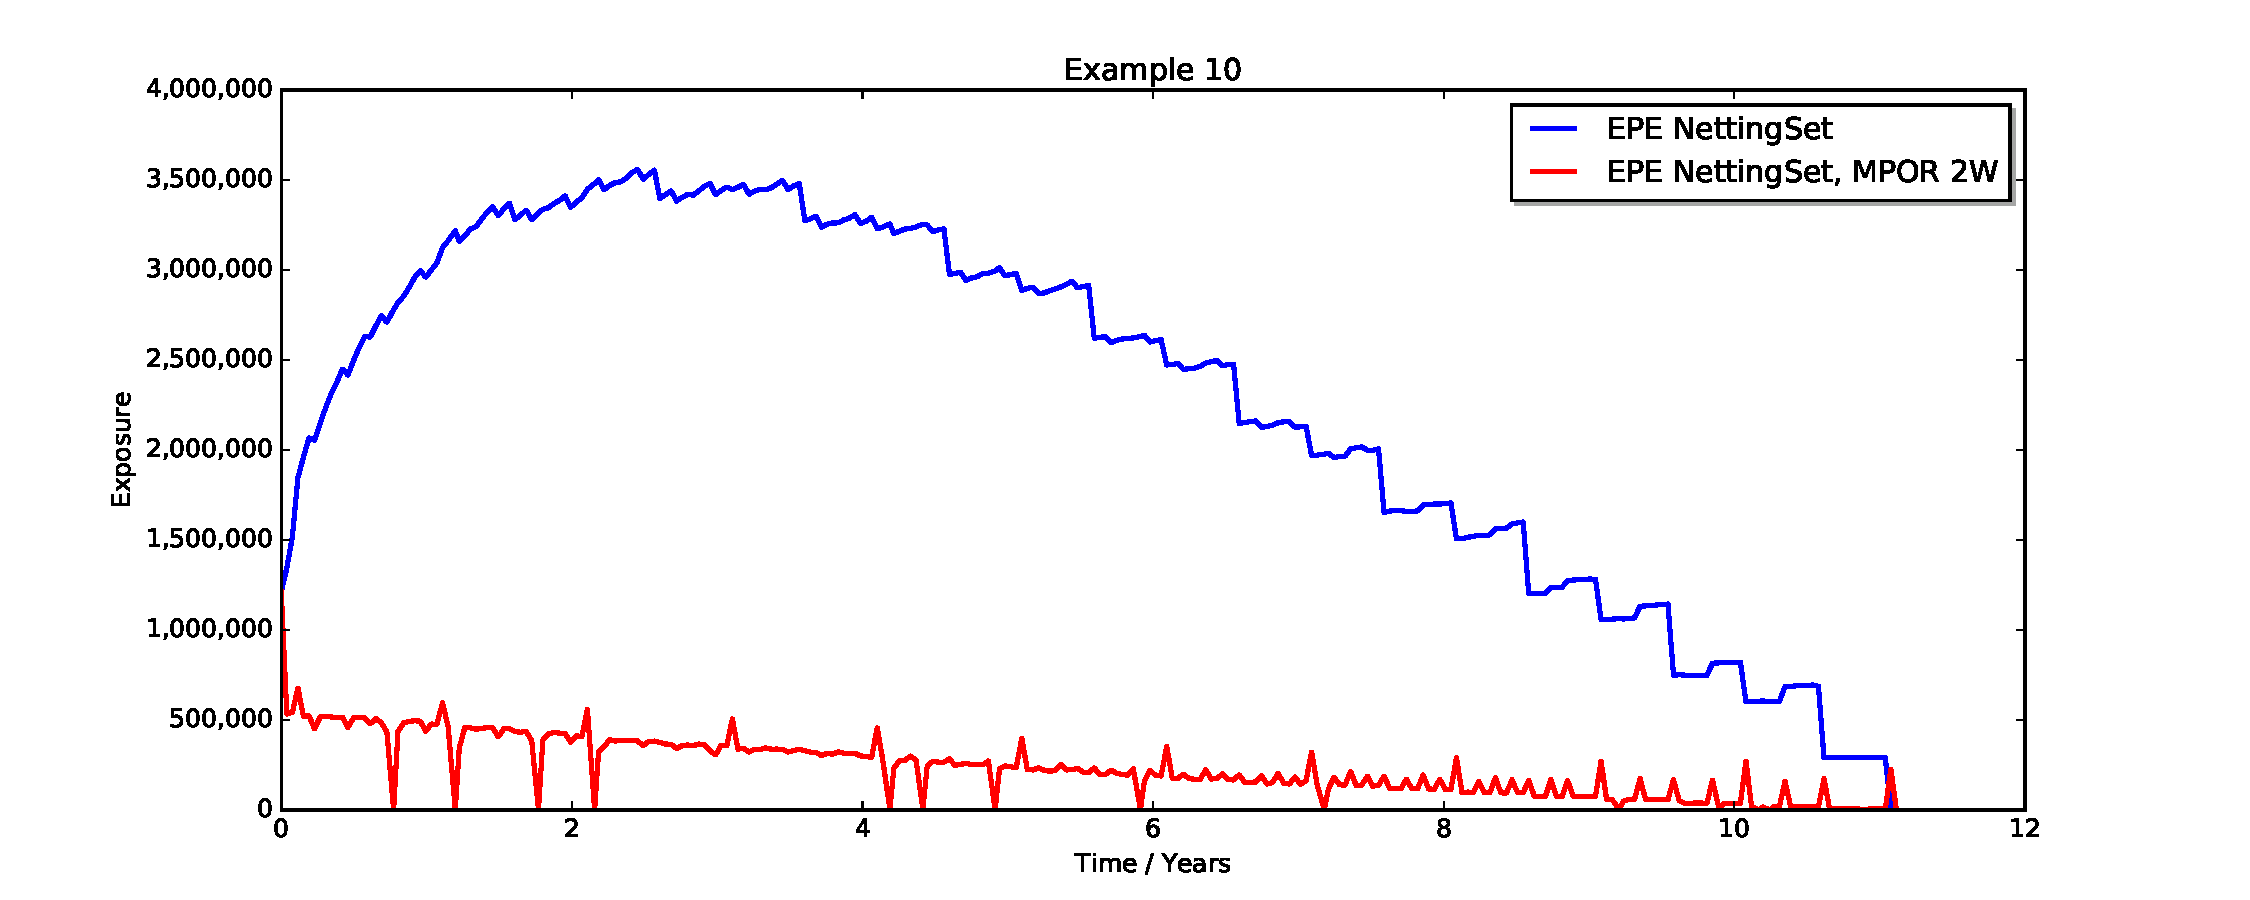
\includegraphics[scale=0.45]{examples/mpl_mpor_epe.pdf}
\end{center}
\caption{Three Swaps, THR=MTA=0, MPOR=2w. Simulation with 5000 paths and bi-weekly time steps.}
\label{fig_10}
\end{figure}

%--------------------------------------------------------
\subsection*{CVA, DVA, FVA, COLVA, MVA, Collateral Floor}
%--------------------------------------------------------

We use one of the cases in {\tt Examples/Example\_10} to demonstrate the
XVA outputs, see folder {\tt Examples/Example\_10/Output/collateral\_threshold\_dim}.

\medskip The summary of all value adjustments (CVA, DVA, FVA, COLVA, MVA, as well as the Collateral Floor) is provided
in file {\tt xva.csv}.  The file includes the allocated CVA and DVA numbers to individual trades as introduced in the
next section. The following table illustrates the file's layout, omitting the three columns containing allocated data.

\begin{center}
\resizebox{\columnwidth}{!}{%
\begin{tabular}{|l|l|r|r|r|r|r|r|r|r|r|}
\hline
TradeId & NettingSetId & CVA & DVA & FBA & FCA & COLVA & MVA & CollateralFloor & BaselEPE & BaselEEPE \\
\hline
 & CPTY\_A &  6,521  &  151,193  & -946  &  72,103  &  2,769  & -14,203  &  189,936  &  113,260  &  1,211,770 \\
Swap\_1 & CPTY\_A &  127,688  &  211,936  & -19,624  &  100,584  &  n/a  &  n/a  &  n/a   &  2,022,590  &  2,727,010 \\
Swap\_3 & CPTY\_A &  71,315  &  91,222  & -11,270  &  43,370  &  n/a  &  n/a  &  n/a   &  1,403,320  &  2,183,860 \\
Swap\_2 & CPTY\_A &  68,763  &  100,347  & -10,755  &  47,311  &  n/a  &  n/a  &  n/a   &  1,126,520  &  1,839,590 \\
\hline
\end{tabular}
}
\end{center}

The line(s) with empty TradeId column contain values at netting set level, the others contain uncollateralised
single-trade VAs.  Note that COLVA, MVA and Collateral Floor are only available at netting set level at which collateral
is posted.

\medskip
Detailed output is written for COLVA and Collateral Floor to file {\tt colva\_nettingset\_*.csv} which shows the 
incremental contributions to these two VAs through time.


%--------------------------------------------------------
\subsection*{Exposure Reports \& XVA Allocation to Trades}
%--------------------------------------------------------
Using the example in folder {\tt Examples/Example\_10} we illustrate here the layout of an exposure report produced by
ORE. The report shows the exposure evolution of Swap\_1 without collateral which - after running Example\_10 - is found
in folder \\
{\tt Examples/Example\_10/Output/collateral\_none/exposure\_trade\_Swap\_1.csv}:

\begin{center}
\resizebox{\columnwidth}{!}{%
\begin{tabular}{|l|l|r|r|r|r|r|r|r|r|}
\hline
TradeId & Date & Time & EPE & ENE & AllocEPE & AllocENE & PFE & BaselEE & BaselEEE \\
\hline
Swap\_1 & 05/02/16 & 0.0000 & 0  & 1,711,748  & 0  & 0  & 0  & 0  & 0 \\
Swap\_1 & 19/02/16 & 0.0383 & 38,203   & 1,749,913  & -1,200,677 & 511,033 & 239,504 & 38,202 & 38,202 \\
Swap\_1 & 04/03/16 & 0.0765 & 132,862  & 1,843,837 & -927,499 & 783,476 & 1,021,715 & 132,845 & 132,845 \\
%Swap\_1 & 18/03/16 & 0.1148 & 299,155  & 1,742,450  & -650,225  & 793,067  & 1,914,150  & 299,091  & 299,091 \\
%Swap\_1 & 01/04/16 & 0.1530 & 390,178  & 1,834,810  & -552,029  & 892,604  & 2,373,560  & 390,058  & 390,058 \\
%Swap\_1 & 15/04/16 & 0.1913 & 471,849  & 1,918,600  & -465,580  & 981,171  & 2,765,710  & 471,659  & 471,659 \\
%Swap\_1 & 29/04/16 & 0.2295 & 550,301  & 2,000,640  & -330,578  & 1,119,760  & 3,106,810  & 550,016  & 550,016 \\
%Swap\_1 & 13/05/16 & 0.2678 & 620,279  & 2,074,880  & -266,042  & 1,188,560  & 3,427,080  & 619,888  & 619,888 \\
%Swap\_1 & 27/05/16 & 0.3060 & 690,018  & 2,140,320  & -190,419  & 1,259,880  & 3,778,570  & 689,509  & 689,509 \\
%Swap\_1 & 10/06/16 & 0.3443 & 763,207  & 2,206,020  & -137,681  & 1,305,130  & 4,052,870  & 762,560  & 762,560 \\
Swap\_1 & ... & ...& ... & ... & ... & ... & ... & ... & ... \\
\hline
\end{tabular}
}
\end{center}

The exposure measures EPE, ENE and PFE, the Basel exposure measures $EE_B$ and $EEE_B$, as well as allocated exposures
are defined in \cite{methods}. The PFE quantile and allocation method are chosen as described in section \ref{sec:analytics}. \\

In addition to single trade exposure files, ORE produces an exposure file per netting set. The example from the same
folder as above is:

\begin{center}
\resizebox{\columnwidth}{!}{%
\begin{tabular}{|l|l|r|r|r|r|r|r|r|}
\hline
NettingSet & Date & Time & EPE & ENE & PFE & ExpectedCollateral & BaselEE & BaselEEE \\
\hline
CPTY\_A & 05/02/16 & 0.0000 & 1,203,836 & 0 & 1,203,836 & 0 & 1,203,836 & 1,203,836 \\%1,211,770 & 0 & 1,211,770 & 0 & 1,211,770 & 1,211,770\\
CPTY\_A & 19/02/16 & 0.0383 & 1,337,713 & 137,326 & 3,403,460 & 0 & 1,337,651 & 1,337,651 \\ %0.0383 & 1,344,220 & 137,776 & 3,414,000 & 0 & 1,344,160 & 1,344,160\\
%CPTY\_A & 04/03/16 & 0.0765 & 1,518,610 & 308,381 & 4,354,060 & 0 & 1,518,410 & 1,518,410\\
%CPTY\_A & 18/03/16 & 0.1148 & 1,846,900 & 382,068 & 5,200,730 & 0 & 1,846,500 & 1,846,500\\
%CPTY\_A & 01/04/16 & 0.1530 & 1,961,290 & 494,416 & 5,869,470 & 0 & 1,960,690 & 1,960,690\\
%CPTY\_A & 15/04/16 & 0.1913 & 2,067,240 & 598,283 & 6,384,140 & 0 & 2,066,400 & 2,066,400\\
%CPTY\_A & 29/04/16 & 0.2295 & 2,053,670 & 745,960 & 6,740,070 & 0 & 2,052,610 & 2,066,400\\
%CPTY\_A & 13/05/16 & 0.2678 & 2,149,190 & 845,507 & 6,930,230 & 0 & 2,147,840 & 2,147,840\\
%CPTY\_A & 27/05/16 & 0.3060 & 2,235,630 & 930,218 & 7,295,440 & 0 & 2,233,980 & 2,233,980\\
%CPTY\_A & 10/06/16 & 0.3443 & 2,314,470 & 1,014,690 & 7,753,190 & 0 & 2,312,510 & 2,312,510\\
CPTY\_A & ... & ...& ... & ... & ... & ... & ... & ...\\
%CPTY\_A & 07/07/17 & 1.4167 & 3,320,430 & 2,423,890 & 12,787,900 & 0 & 3,304,650 & 3,304,650\\
%CPTY\_A & 21/07/17 & 1.4551 & 3,351,780 & 2,452,640 & 12,964,200 & 0 & 3,335,420 & 3,335,420\\
%CPTY\_A & 04/08/17 & 1.4934 & 3,302,820 & 2,511,500 & 12,796,100 & 0 & 3,286,260 & 3,335,420\\
%CPTY\_A & 18/08/17 & 1.5318 & 3,339,840 & 2,545,850 & 13,120,000 & 0 & 3,322,640 & 3,335,420\\
%CPTY\_A & 01/09/17 & 1.5701 & 3,371,300 & 2,576,100 & 13,238,700 & 0 & 3,353,480 & 3,353,480\\
%CPTY\_A & 15/09/17 & 1.6085 & 3,279,670 & 2,555,370 & 13,041,300 & 0 & 3,261,880 & 3,353,480\\
%CPTY\_A & 29/09/17 & 1.6468 & 3,305,060 & 2,579,200 & 13,072,800 & 0 & 3,286,680 & 3,353,480\\
%CPTY\_A & 13/10/17 & 1.6852 & 3,332,830 & 2,604,200 & 13,225,600 & 0 & 3,313,850 & 3,353,480\\
%CPTY\_A & 27/10/17 & 1.7236 & 3,280,280 & 2,661,770 & 13,034,600 & 0 & 3,261,150 & 3,353,480\\
%CPTY\_A & 13/11/17 & 1.7701 & 3,316,800 & 2,701,060 & 13,331,600 & 0 & 3,296,880 & 3,353,480\\
%CPTY\_A & 24/11/17 & 1.8003 & 3,337,760 & 2,720,870 & 13,402,400 & 0 & 3,317,280 & 3,353,480\\
%CPTY\_A & ... & ...& ... & ... & ... & ... & ... & ...\\
\hline
\end{tabular}
}
\end{center}

Allocated exposures are missing here, as they make sense at the trade level only, and the expected collateral balance is
added for information (in this case zero as collateralisation is deactivated in this example).

\medskip The allocation of netting set exposure and XVA to the trade level is frequently required by finance
departments. This allocation is also featured in {\tt Examples/Example\_10}. We start again with the uncollateralised
case in figure \ref{fig_12}, followed by the case with threshold 1m EUR in figure \ref{fig_13}.
\begin{figure}[h!]
\begin{center}
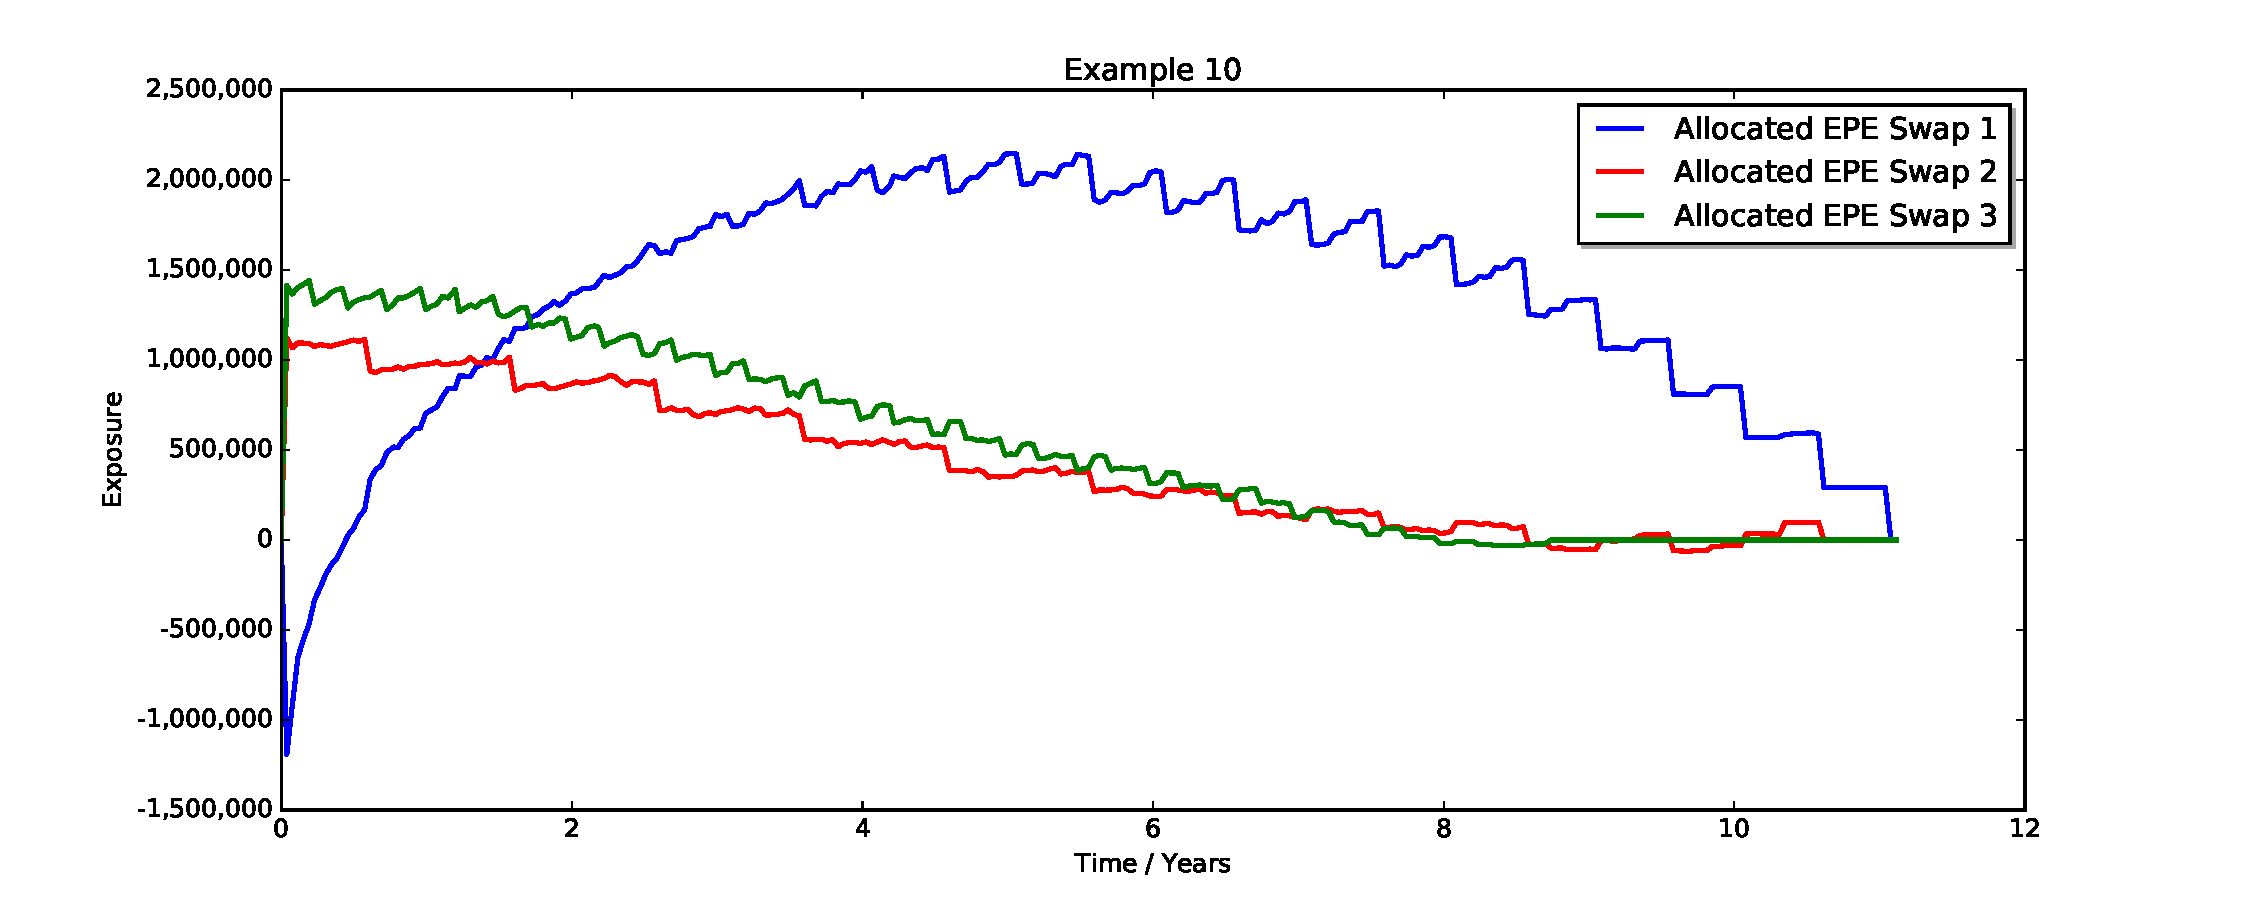
\includegraphics[scale=0.45]{examples/mpl_nocollateral_allocated_epe.pdf}
\end{center}
\caption{Exposure allocation without collateral. Simulation with 5000 paths and bi-weekly time steps.}
\label{fig_12}
\end{figure}
In both cases we apply the {\em marginal} (Euler) allocation method as published by Pykhtin and Rosen in 2010, hence we
see the typical negative EPE for one of the trades at times when it reduces the netting set exposure. The case with
collateral moreover shows the typical spikes in the allocated exposures.
\begin{figure}[h!]
\begin{center}
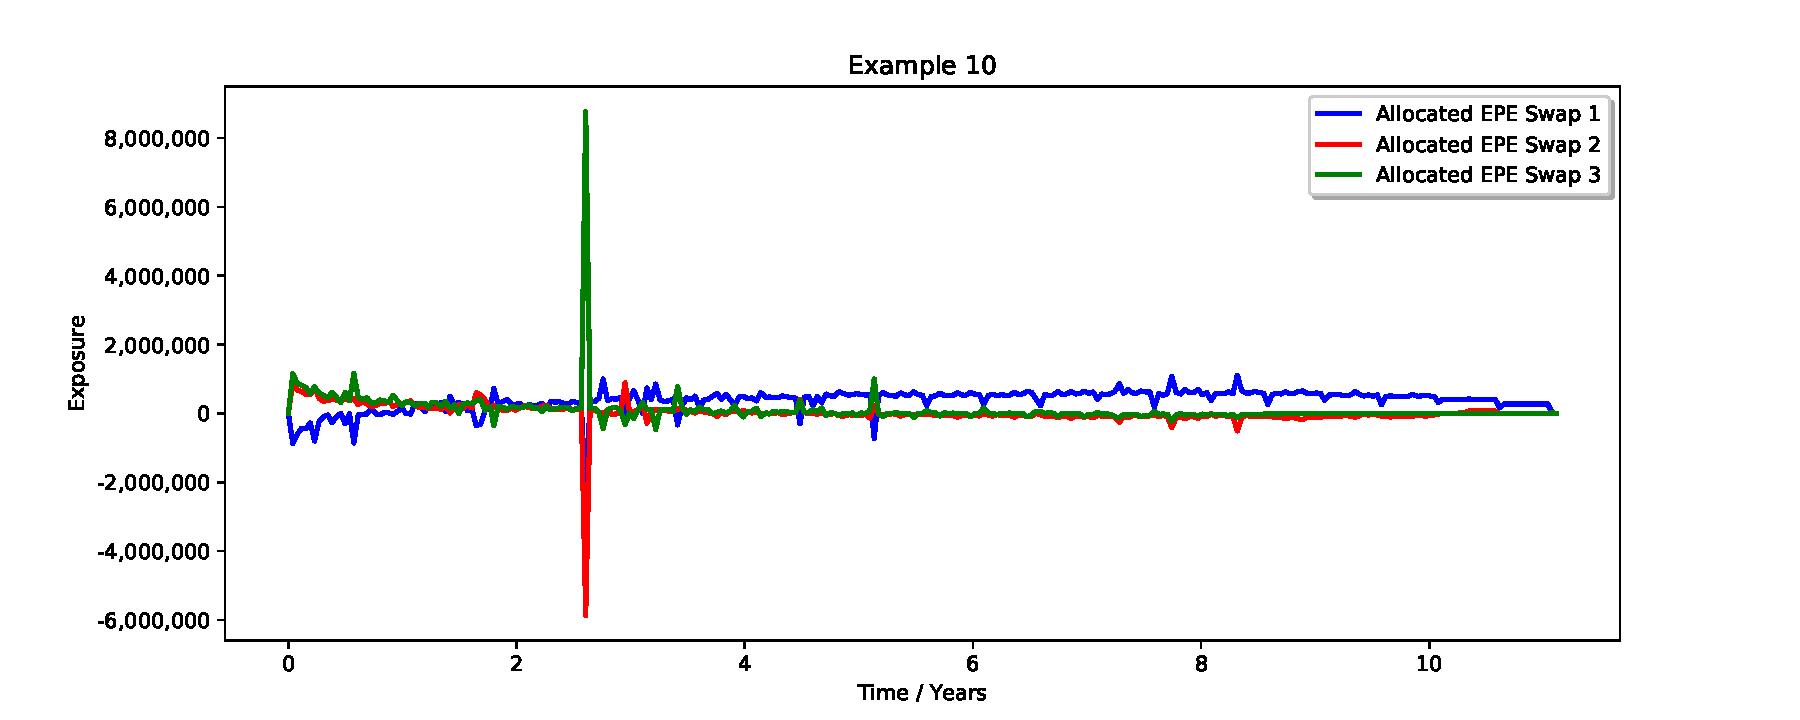
\includegraphics[scale=0.45]{examples/mpl_threshold_allocated_epe.pdf}
\end{center}
\caption{Exposure allocation with collateral and threshold 1m EUR. Simulation with 5000 paths and bi-weekly time steps.}
\label{fig_13}
\end{figure}
The analytics results also feature allocated XVAs in file {\tt xva.csv} which are derived from the allocated exposure
profiles. Note that ORE also offers alternative allocation methods to the marginal method by Pykhtin/Rosen, which can be
explored with {\tt Examples/Example\_10}.

%--------------------------------------------------------
\subsection{Basel Exposure Measures}\label{sec:basel}
%--------------------------------------------------------

Example {\tt Example\_11} demonstrates the relation between the evolution of the expected exposure (EPE in our notation)
to the `Basel' exposure measures EE\_B, EEE\_B, EPE\_B and EEPE\_B as defined in \cite{methods}. In
particular the latter is used in internal model methods for counterparty credit risk as a measure for the exposure at
default. It is a `derivative' of the expected exposure evolution and defined as a time average over the running maximum
of EE\_B up to the horizon of one year.
\begin{figure}[h!]
\begin{center}
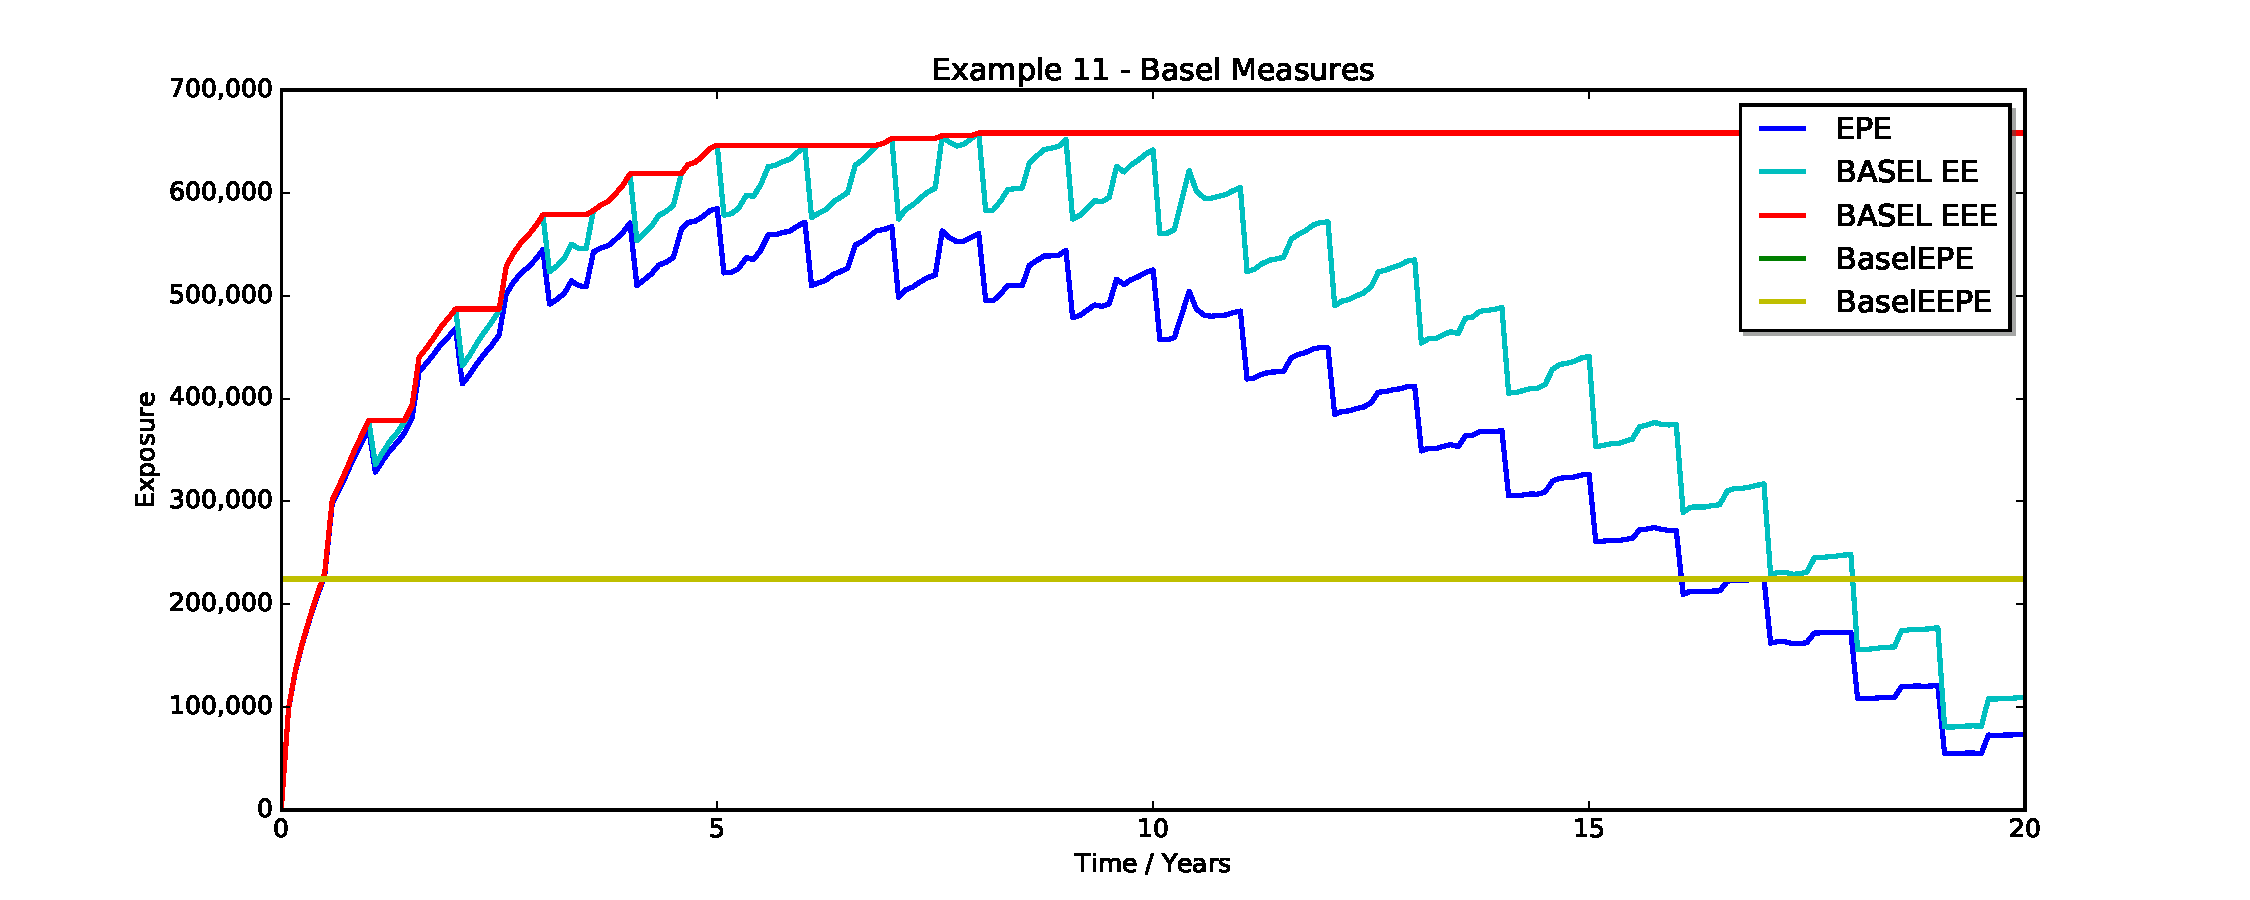
\includegraphics[scale=0.45]{examples/mpl_basel_exposures.pdf}
\end{center}
\caption{Evolution of the expected exposure of Vanilla Swap, comparison to the `Basel' exposure measures EEE\_B, EPE\_B and EEPE\_B. Note that the latter two are indistinguishable in this case, because the expected exposure is increasing for the first year.}
\label{fig_14}
\end{figure}

%--------------------------------------------------------
\subsection{Long Term Simulation with Horizon Shift}\label{sec:longterm}
%--------------------------------------------------------

The example in folder {\tt Example\_12} finally demonstrates an effect that, at first glance, seems to cause a serious
issue with long term simulations. Fortunately this can be avoided quite easily in the Linear Gauss Markov model setting
that is used here. \\

In the example we consider a Swap with maturity in 50 years in a flat yield curve environment. If we simulate this
naively as in all previous cases, we obtain a particularly noisy EPE profile that does not nearly reconcile with the
known exposure (analytical Swaption prices). This is shown in figure \ref{fig_15} (`no horizon shift'). The origin of
this issue is the width of the risk-neutral NPV distribution at long time horizons which can turn out to be quite small
so that the Monte Carlo simulation with finite number of samples does not reach far enough into the positive or negative
NPV range to adequately sample the distribution, and estimate both EPE and ENE in a single run.  Increasing the number
of samples may not solve the problem, and may not even be feasible in a realistic setting. \\

The way out is applying a `shift transformation' to the Linear Gauss Markov model, see {\tt
  Example\_12/Input/simulation2.xml} in lines 92-95:
\begin{listing}[H]
%\hrule\medskip
\begin{minted}[fontsize=\footnotesize]{xml}
        <ParameterTransformation>
          <ShiftHorizon>30.0</ShiftHorizon>
          <Scaling>1.0</Scaling>
        </ParameterTransformation>
\end{minted}
%\hrule
%\caption{LGM Shift transformation}
%\label{lst:shift_transformation}
\end{listing}

The effect of the 'ShiftHorizon' parameter $T$ is to apply a shift to the Linear Gauss Markov model's $H(t)$ parameter
(see \cite{methods}) {\em after} the model has been calibrated, i.e. to replace:
$$ 
H(t) \rightarrow H(t) - H(T) 
$$ 
It can be shown that this leaves all expectations computed in the model (such as EPE and ENE) invariant. As explained in
\cite{Lichters}, subtracting an $H$ shift effectively means performing a change of measure from the `native' LGM measure
to a T-Forward measure with horizon $T$, here 30 years. Both negative and positive shifts are permissible, but only
negative shifts are connected with a T-Forward measure and improve numerical stability. \\

In our experience it is helpful to place the horizon in the middle of the portfolio duration to significantly improve
the quality of long term expectations. The effect of this change (only) is shown in the same figure \ref{fig_15}
(`shifted horizon').
\begin{figure}[h!]
\begin{center}
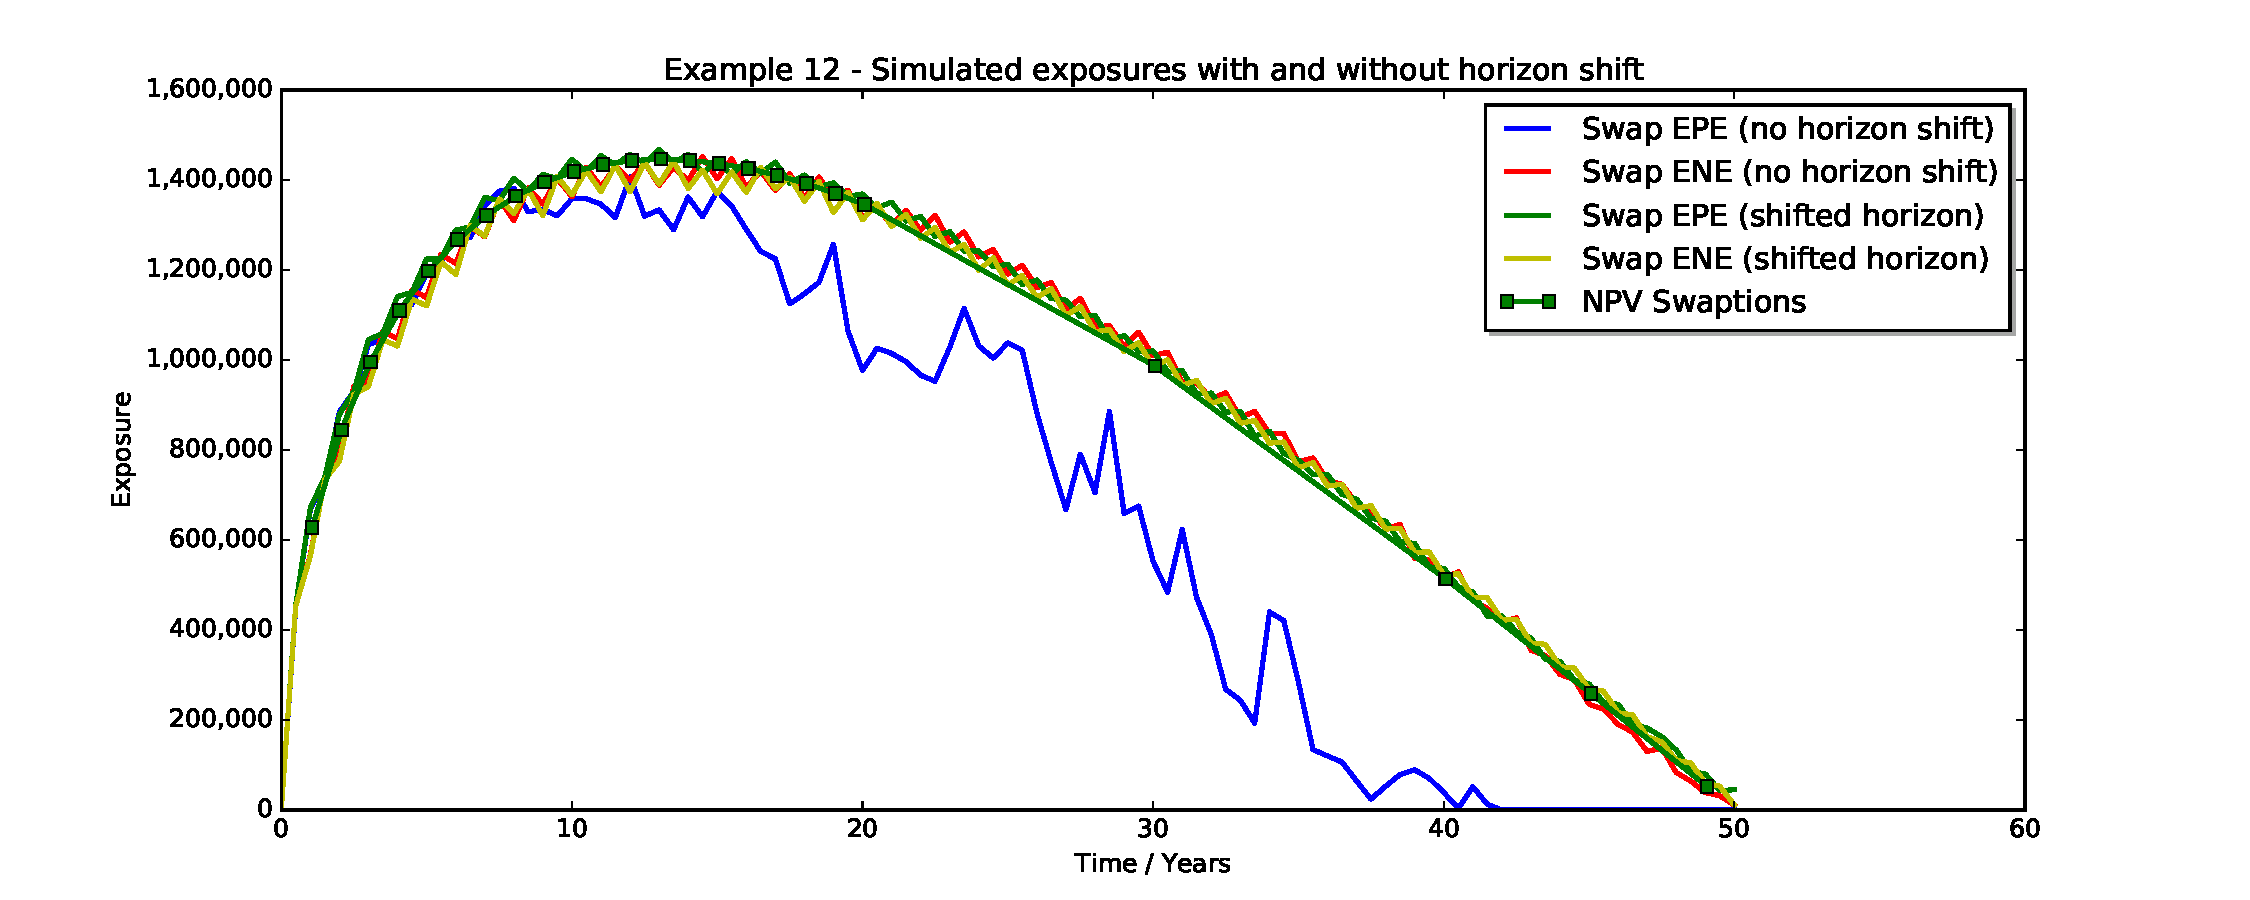
\includegraphics[scale=0.45]{examples/mpl_longterm.pdf}
\end{center}
\caption{Long term Swap exposure simulation with and without horizon shift.}
\label{fig_15}
\end{figure}
Figure \ref{fig_15b} further illustrates the origin of the problem and its resolution: The rate distribution's mean
(without horizon shift or change of measure) drifts upwards due to convexity effects (note that the yield curve is flat
in this example), and the distribution's width is then too narrow at long horizons to yield a sufficient number of low
rate scenarios with contributions to the Swap's $\EPE$ (it is a floating rate payer). With the horizon shift (change of
measure), the distribution's mean is pulled 'back' at long horizons, because the convexity effect is effectively wiped
out at the chosen horizon, and the expected rate matches the forward rate.

\begin{figure}[h!]
\begin{center}
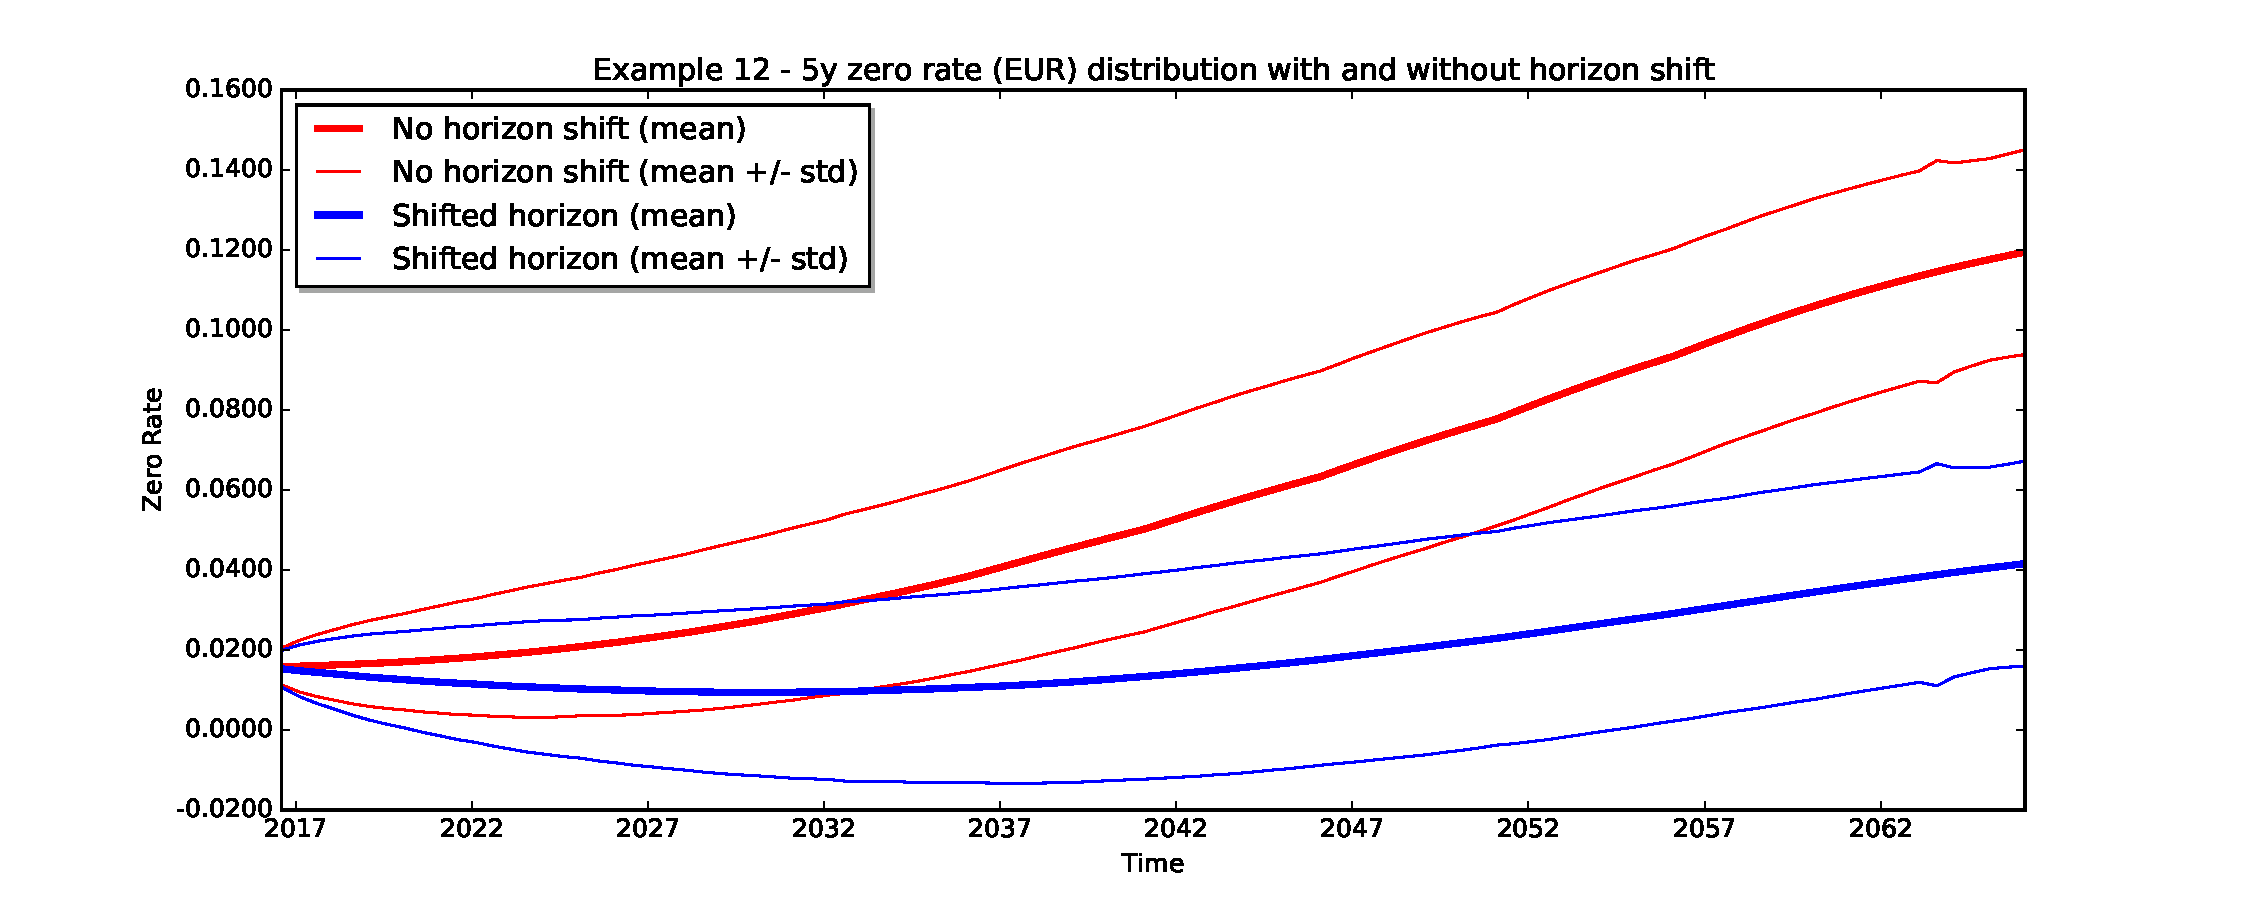
\includegraphics[scale=0.45]{examples/mpl_rates.pdf}
\end{center}
\caption{Evolution of rate distributions with and without horizon shift (change of measure). Thick lines indicate mean
  values, thin lines are contours of the rate distribution at $\pm$ one standard deviation.}
\label{fig_15b}
\end{figure}

%--------------------------------------------------------
\subsection{Dynamic Initial Margin and MVA}\label{sec:dim}
%--------------------------------------------------------

This example in folder {\tt Examples/Example\_13} demonstrates Dynamic Initial Margin calculations (see also \cite{methods}) for a number of elementary products:
\begin{itemize}
\item A single currency Swap in EUR (case A), 
\item a European Swaption in EUR with physical delivery (case B), 
\item a single currency Swap in USD (case C),
\item a EUR/USD cross currency Swap (case D),
\item a EUR/USD FX Option (case E).
\end{itemize}

The examples can be run as before with 

\medskip
\centerline{\tt python run\_A.py} 

\medskip
and likewise for cases B--E. The essential results of each run are visualised in the form of 
\begin{itemize}
\item evolution of expected DIM which feeds into the MVA calculation
\item regression plots at selected future times 
\end{itemize}
illustrated for cases A, B and E in figures \ref{fig_ex13a_evolution} - \ref{fig_ex13c_evolution}. 

\begin{figure}[h!]
\begin{center}
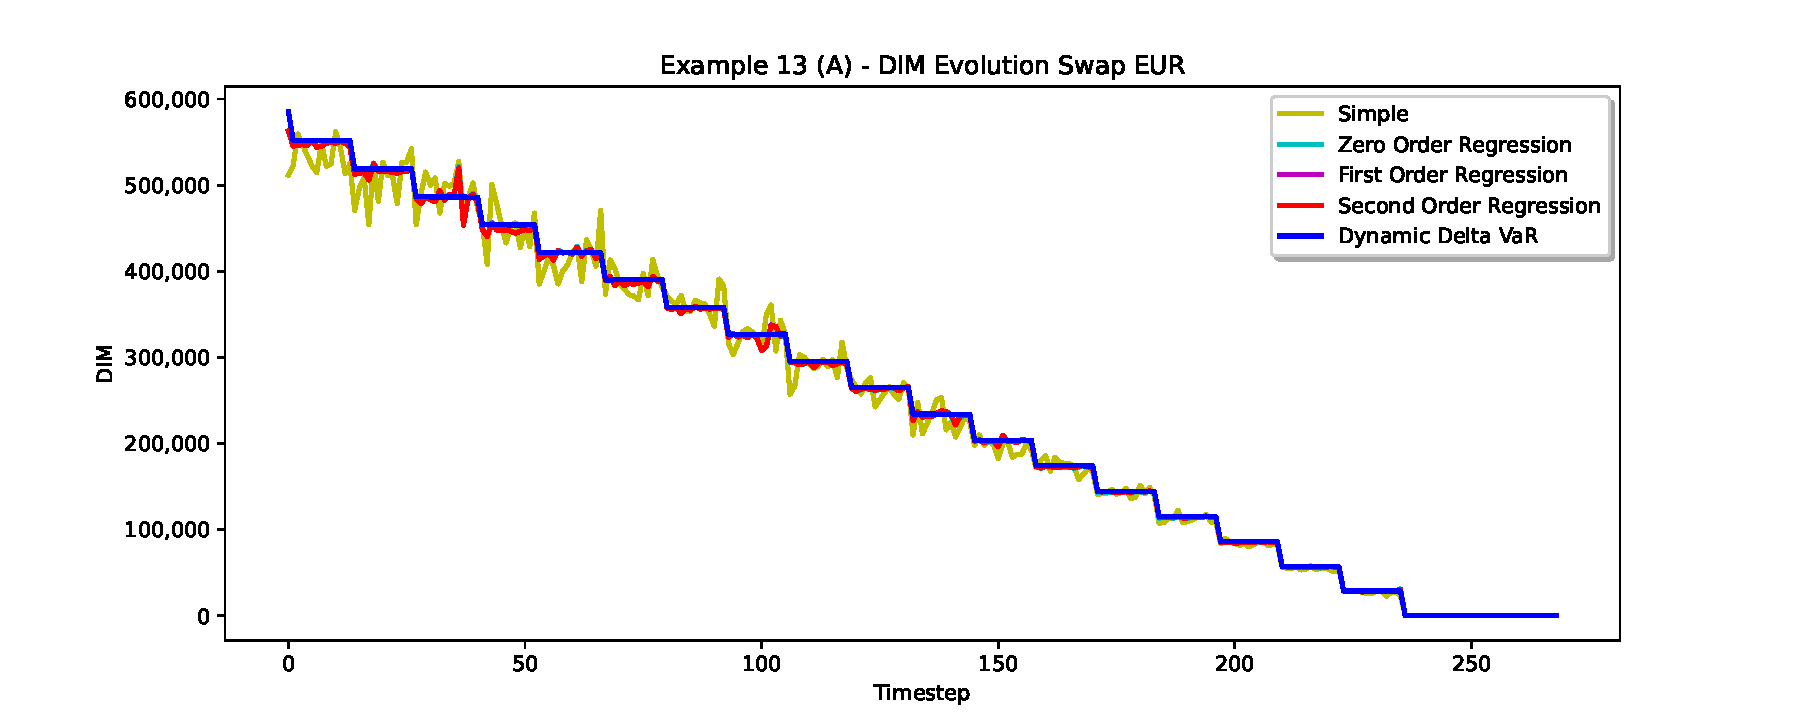
\includegraphics[scale=0.45]{examples/mpl_dim_evolution_A_swap_eur.pdf}
\end{center}
\caption{Evolution of expected Dynamic Initial Margin (DIM) for the EUR Swap of Example 13 A. Regression DIM is evaluated using
  regression of NPV change variances versus the simulated 3M Euribor fixing; regression polynomials are zero, first and
  second order (first and second order curves are not noticebly different in this case). The simulation uses 1000 samples and a time
  grid with bi-weekly steps in line with the Margin Period of Risk.}
\label{fig_ex13a_evolution}
\end{figure}

\begin{figure}[h!]
\begin{center}
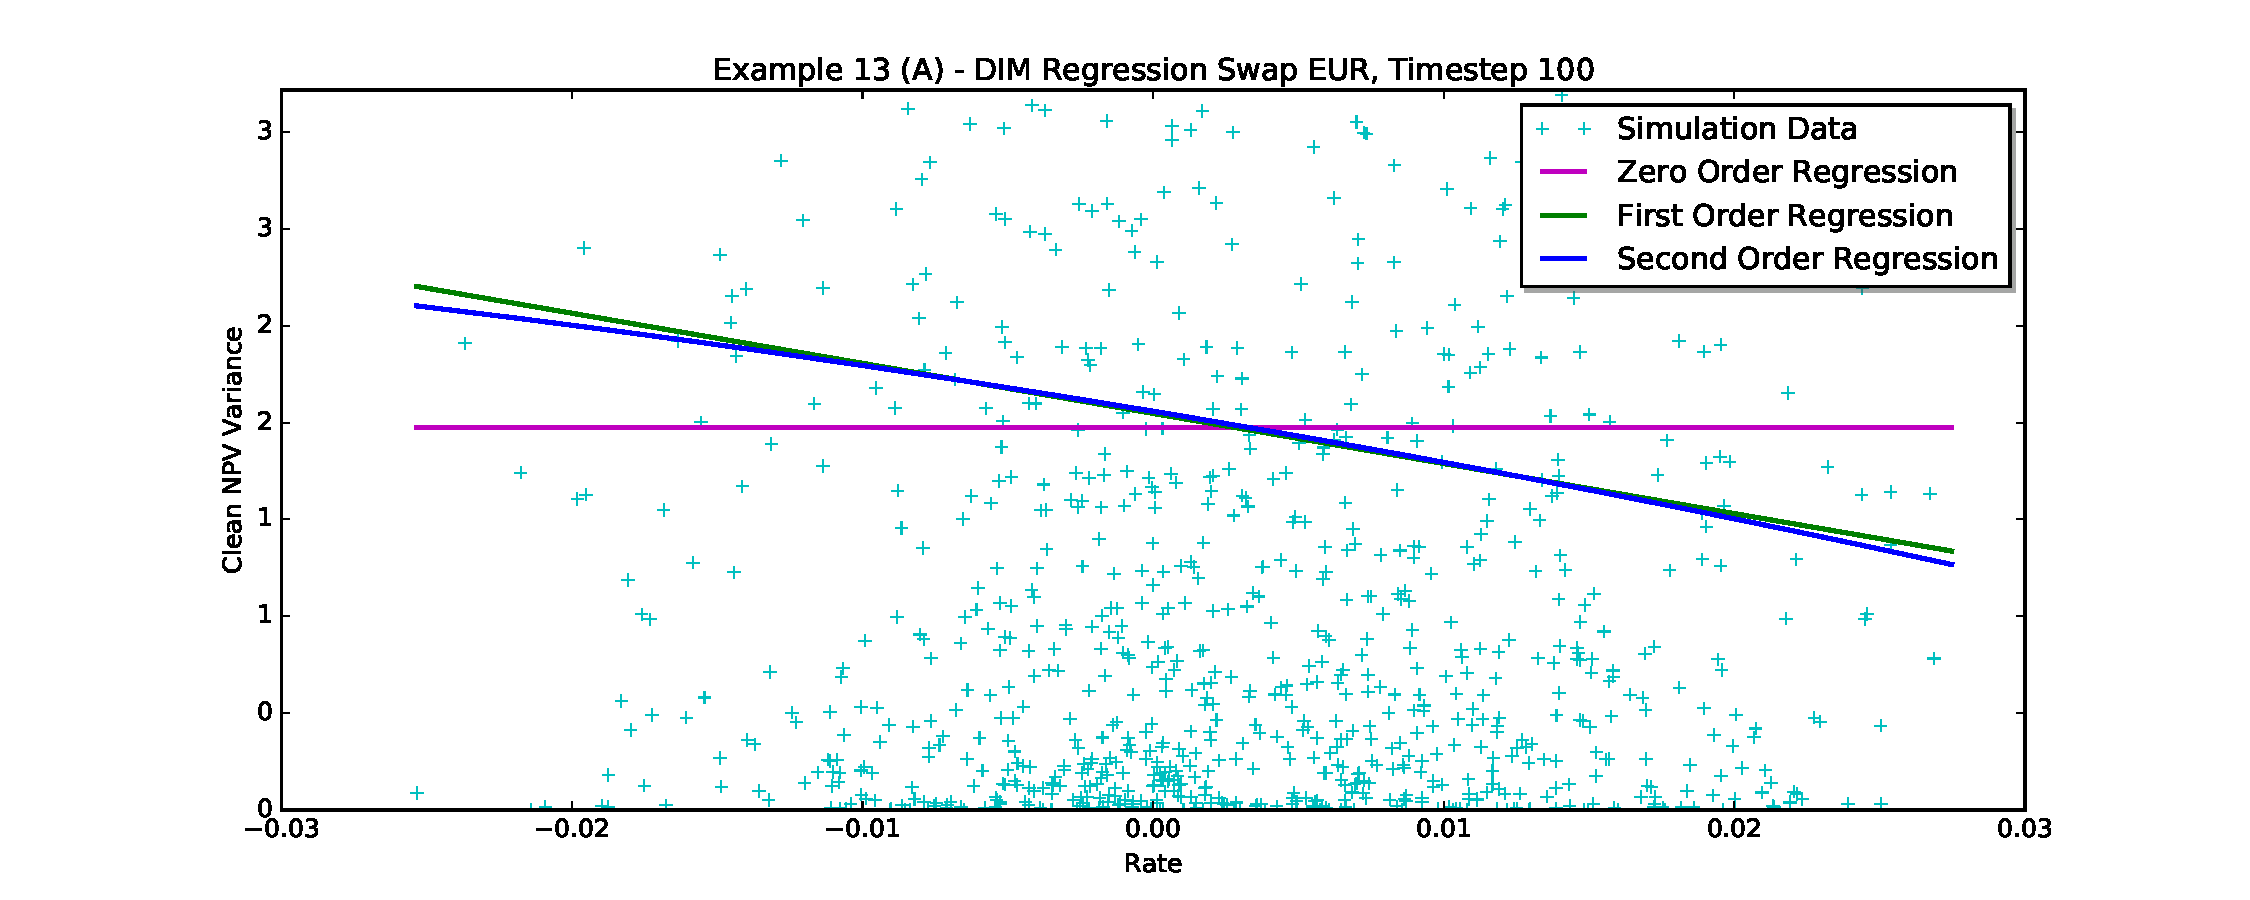
\includegraphics[scale=0.45]{examples/mpl_dim_regression_A_swap_eur.pdf}
\end{center}
\caption{Regression snapshot at time step 100 for the EUR Swap of Example 13 A.}
\label{fig_ex13a_regression}
\end{figure}

The DIM evolution graphs compare a subset of the following Initial Margin projections methods in ORE
\begin{itemize}
\item Simple: 99\% quantile of NPV changes ($\Delta$) over the Margin Period of Risk across all paths, i.e. same IM applied across paths
\item Zero Order ``Regression'': Standard deviation of $\Delta$s scaled to the 99\% quantile with factor 2.33 (normal distribution assumption); same IM applied across paths
\item First/Second Order Regression: Conditional standard deviation of $\Delta$ computed by polynomial first/second order regression of $\Delta$ variances, scaled to the 99\% quantile as avove; different IM amounts applied across paths, graphs show the expected DIM i.e. avergae across paths
\item Dynamic Delta VaR: 99\% quantile VaR based on analytic deltas and vegas computed under scenarios; different IM amounts applied across paths, graphs show the expected DIM i.e. average across paths
\end{itemize}

For a discussion of the regression model performance see \cite{Anfuso2016,LichtersEtAl}. The cases A--E are associated with
various ORE master input files {\tt Input/ore\_A*.xml},  {\tt Input/ore\_B*.xml}, ..., which demonstrate the required simulation
and xva analytic configurations.
 
\begin{figure}[h!]
\begin{center}
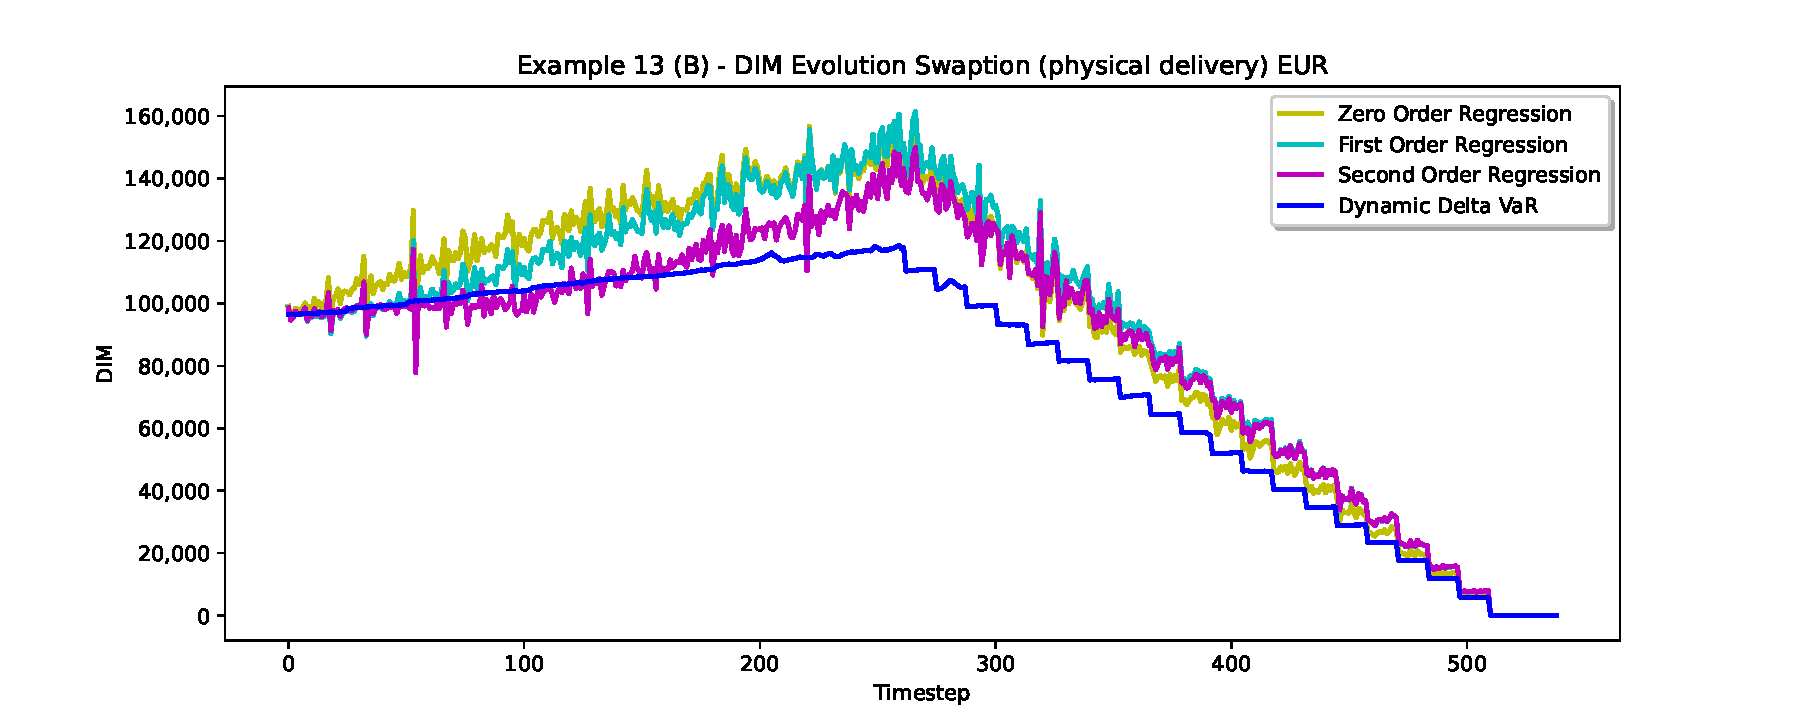
\includegraphics[scale=0.45]{examples/mpl_dim_evolution_B_swaption_eur.pdf}
\end{center}
\caption{Evolution of expected Dynamic Initial Margin (DIM) for the EUR Swaption of Example 13 B with expiry in 10Y
  around time step 100.}
\label{fig_ex13b_evolution}
\end{figure}

\begin{figure}[h!]
\begin{center}
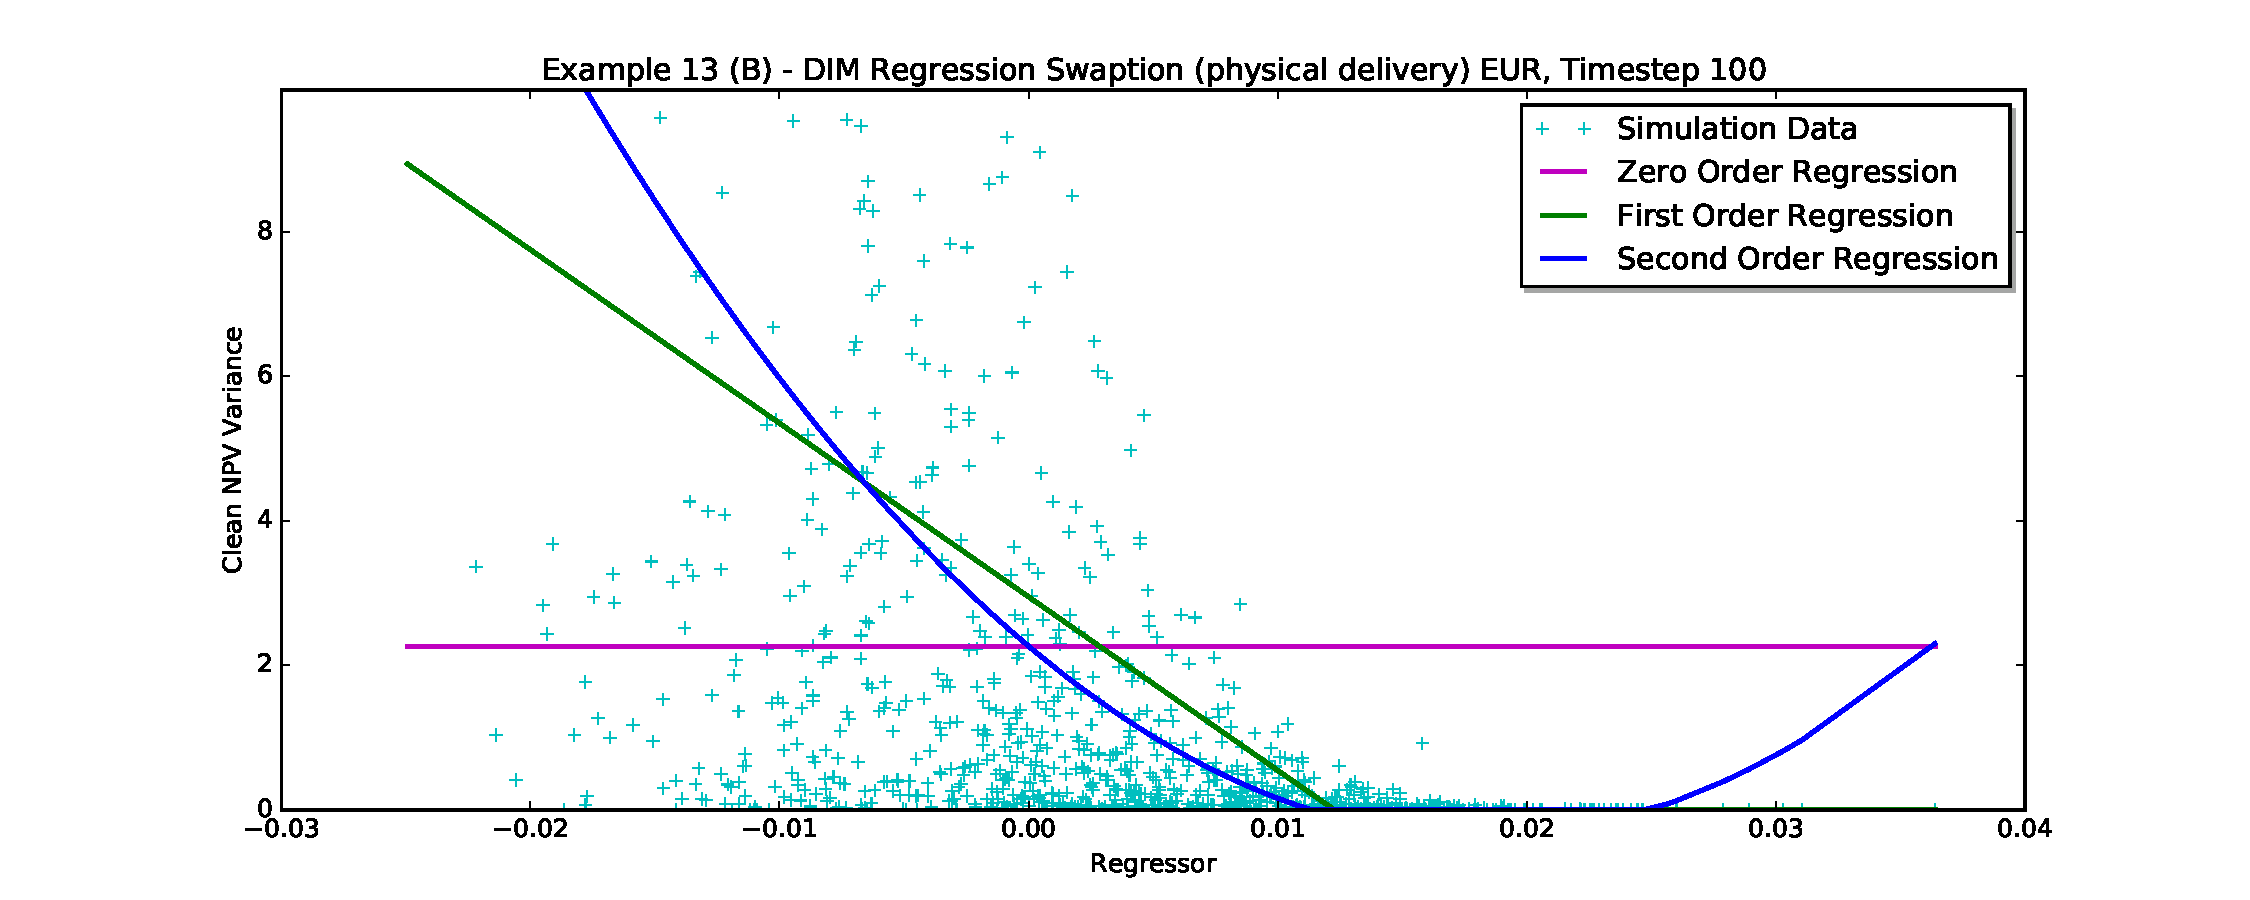
\includegraphics[scale=0.45]{examples/mpl_dim_regression_B_swaption_eur_t100.pdf}
\end{center}
\caption{Regression snapshot at time step 100 (before expiry) for the EUR Swaption of Example 13 B.}
\label{fig_ex13b_regression}
\end{figure}

\begin{figure}[h!]
\begin{center}
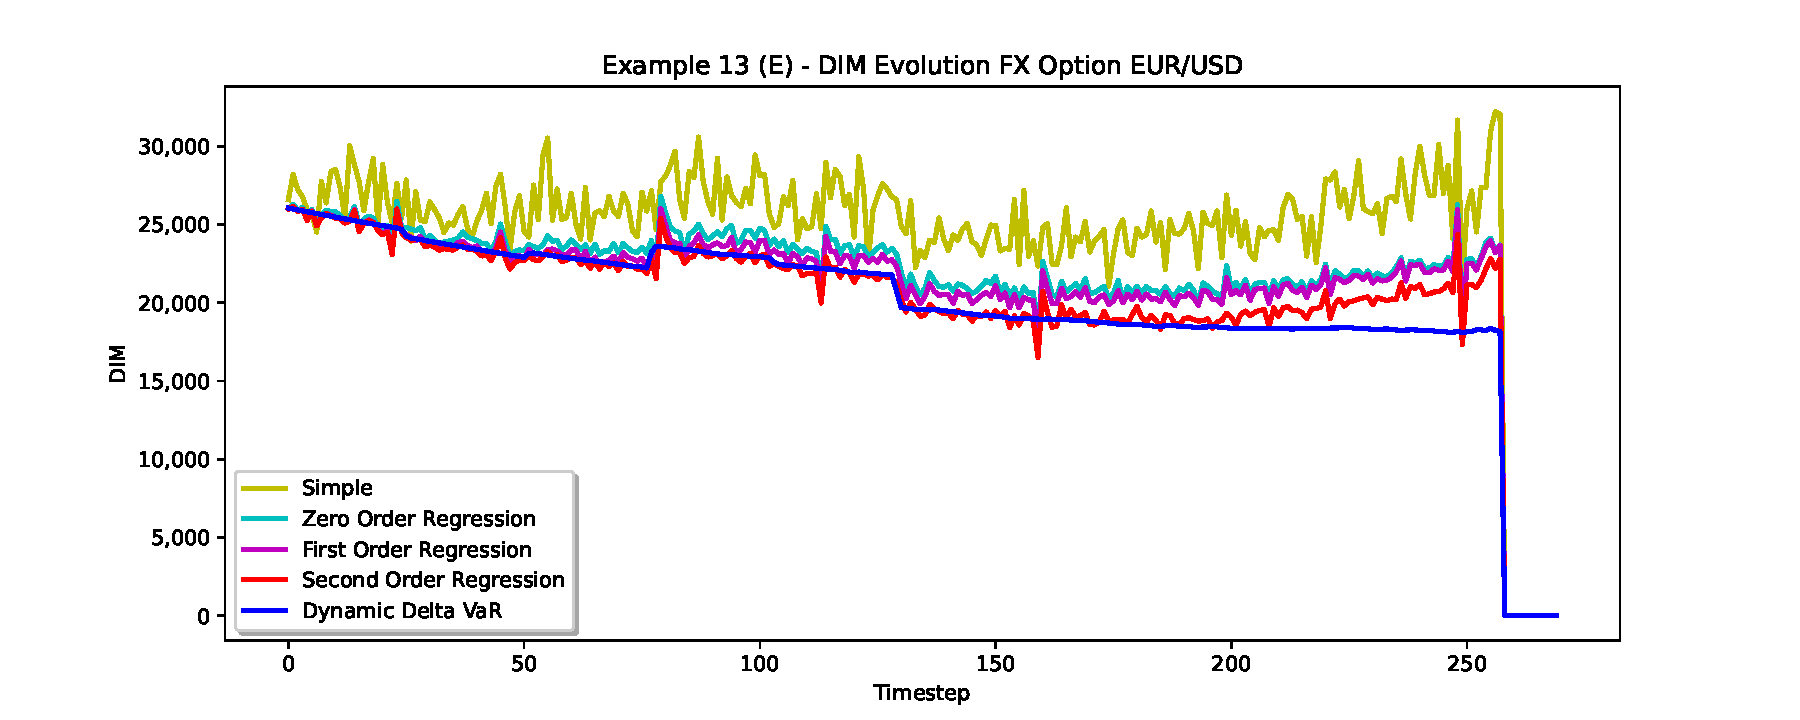
\includegraphics[scale=0.45]{examples/mpl_dim_evolution_E_fxopt.pdf}
\end{center}
\caption{Evolution of expected Dynamic Initial Margin (DIM) for the EUR/USD FX Option of Example 13 (case E) with expiry in 10Y
  around time step 100.}
\label{fig_ex13c_evolution}
\end{figure}

%--------------------------------------------------------
\subsection{Minimal Market Data Setup}
%--------------------------------------------------------

The example in folder {\tt Examples/Example\_14} demonstrates using a minimal market data setup in order to rerun the vanilla Swap exposure simulation shown in {\tt Examples/Example\_1}. The minimal market data uses single points per curve where possible.

%--------------------------------------------------------
\subsection{Sensitivity Analysis, Stress Testing and Parametric Value-at-Risk}
\label{ex:sensitivity_stress}
%--------------------------------------------------------

The example in folder {\tt Examples/Example\_15} demonstrates the calculation of sensitivities and stress scenarios. The
portfolio used in this example consists of

\begin{itemize}
\item a vanilla swap in EUR
\item a cross currency swap EUR-USD
\item a resettable cross currency swap EUR-USD
\item a FX forward EUR-USD
\item a FX call option on USD/GBP % commented out?
\item a FX put option on USD/EUR
\item an European swaption
\item a Bermudan swaption 
\item a cap and a floor in USD
\item a cap and a floor in EUR
\item a fixed rate bond
\item a floating rate bond with floor
\item an Equity call option, put option and forward on S\&P500
\item an Equity call option, put option and forward on Lufthansa
\item a CPI Swap referencing UKRPI
\item a Year-on-Year inflation swap referencing EUHICPXT
\item a USD CDS.
\end{itemize}

The sensitivity configuration in {\tt sensitivity.xml} aims at computing the following sensitivities

\begin{itemize}
\item discount curve sensitivities in EUR, USD; GBP, CHF, JPY, on pillars 6M, 1Y, 2Y, 3Y, 5Y, 7Y, 10Y, 15Y, 20Y (absolute shift of 0.0001)
\item forward curve sensitivities for EUR-EURIBOR 6M and 3M indices, EUR-EONIA, USD-LIBOR 3M and 6M, GBP-LIBOR 3M and
  6M, CHF-LIBOR-6M and JPY-LIBOR-6M indices (absolute shift of 0.0001)
\item yield curve shifts for a bond benchmark curve in EUR (absolute shift of 0.0001)
\item FX spot sensitivities for USD, GBP, CHF, JPY against EUR as the base currency (relative shift of 0.01)
\item FX vegas for USDEUR, GBPEUR, JPYEUR volatility surfaces (relative shift of 0.01)
\item swaption vegas for the EUR surface on expiries 1Y, 5Y, 7Y, 10Y and underlying terms 1Y, 5Y, 10Y (relative shift of 0.01)
\item caplet vegas for EUR and USD on an expiry grid 1Y, 2Y, 3Y, 5Y, 7Y, 10Y and strikes 0.01, 0.02, 0.03, 0.04,
  0.05. (absolute shift of 0.0001)
\item credit curve sensitivities on tenors 6M, 1Y, 2Y, 5Y, 10Y (absolute shift of 0.0001).
\item Equity spots for S\&P500 and Lufthansa
\item Equity vegas for S\&P500 and Lufthansa at expiries 6M, 1Y, 2Y, 3Y, 5Y
\item Zero inflation curve deltas for UKRPI and EUHICPXT at tenors 6M, 1Y, 2Y, 3Y, 5Y, 7Y, 10Y, 15Y, 20Y
\item Year on year inflation curve deltas for EUHICPXT at tenors 6M, 1Y, 2Y, 3Y, 5Y, 7Y, 10Y, 15Y, 20Y
\end{itemize}

Furthermore, mixed second order derivatives (``cross gammas'') are computed for discount-discount, discount-forward and
forward-forward curves in EUR.

By definition the sensitivities are zero rate sensitivities and optionlet sensitivities, no par sensitivities are
provided. The sensitivity analysis produces three output files.

The first, {\tt scenario.csv}, contains the shift
direction ({\tt UP}, {\tt DOWN}, {\tt CROSS}), the base NPV, the scenario NPV and the difference of these two for each
trade and sensitivity key. For an overview over the possible scenario keys see \ref{sec:sensitivity}.

The second file, {\tt sensitivity.csv}, contains the shift size (in absolute terms always) and first (``Delta'') and second
(``Gamma'') order finite differences computed from the scenario results. Note that the Delta and Gamma results are pure
differences, i.e. they are not divided by the shift size.

The second file also contains second order mixed differences according to the specified cross gamma filter, along with the shift sizes for the two factors involved.

The stress scenario definition in {\tt stresstest.xml} defines two stress tests:

\begin{itemize}
\item {\tt parallel\_rates}: Rates are shifted in parallel by 0.01 (absolute). The EUR bond benchmark curve is shifted by
  increasing amounts 0.001, ..., 0.009 on the pillars 6M, ..., 20Y. FX Spots are shifted by 0.01 (relative), FX vols by
  0.1 (relative), swaption and cap floor vols by 0.0010 (absolute).
  Credit curves are not yet shifted.
\item {\tt twist}: The EUR bond benchmark curve is shifted by amounts -0.0050, -0.0040, -0.0030, -0.0020, 0.0020,
  0.0040, 0.0060, 0.0080, 0.0100 on pillars 6M, 1Y, 2Y, 3Y, 5Y, 7Y, 10Y, 15Y, 20Y.
\end{itemize}

The corresponding output file {\tt stresstest.csv} contains the base NPV, the NPV under the scenario shifts and the
difference of the two for each trade and scenario label.

%\todo[inline]{Update after CDS has been added to the example.}
\medskip
Finally, this example demonstrates a parametric VaR calculation based on the sensitivity and cross gamma output from the sensitivity analysis (deltas, vegas, gammas, cross gammas) and an external covariance matrix input. The result in {\tt var.csv} shows a breakdown by portfolio, risk class (All, Interest Rate, FX, Inflation, Equity, Credit) and risk type (All, Delta \& Gamma, Vega). The results shown are Delta Gamma Normal VaRs for the 95\% and 99\% quantile, the holding period is incorporated into the input covariances. Alternatively, one can choose a Monte Carlo VaR which means that the sensitivity based P\&L distribution is evaluated with MC simulation assuming normal respectively log-normal risk factor distribution. 
 
%--------------------------------------------------------
\subsection{Equity Derivatives Exposure}\label{ex:equityderivatives}
%--------------------------------------------------------

The example in folder {\tt Examples/Example\_16} demonstrates the computation of NPV, sensitivities, exposures and XVA for a portfolio 
of OTC equity derivatives. The portfolio used in this example consists of:

\begin{itemize}
	\item an equity call option denominated in EUR (``Luft'')
	\item an equity put option denominated in EUR (``Luft'')
	\item an equity forward denominated in EUR (``Luft'')
	\item an equity call option denominated in USD (``SP5'')
	\item an equity put option denominated in USD (``SP5'')
	\item an equity forward denominated in USD (``SP5'')
	\item an equity Swap in USD with return type  ``price'' (``SP5'')
	\item an equity Swap in USD with return type ``total'' (``SP5'')
\end{itemize}

The step-by-step procedure for running ORE is identical for equities as for other asset classes; the same market and 
portfolio data files are used to store the equity market data and trade details, respectively. For the exposure 
simulation, the calibration parameters for the equity risk factors can be set in the usual {\tt simulation.xml} file.

Looking at the MtM results in the output file {\tt npv.csv} we observe that put-call parity ($V_{Fwd} = V_{Call} - 
V_{Put}$) is observed as expected. Looking at Figure \ref{fig_eq_call} we observe that the Expected Exposure profile of 
the equity call option trade is relatively smooth over time, while for the equity forward trade the Expected Exposure 
tends to increase as we approach maturity. This behaviour is similar to what we observe in sections \ref{sec:fxfwd} 
and \ref{sec:fxoption}. 

\begin{figure}[h!]
	\begin{center}
		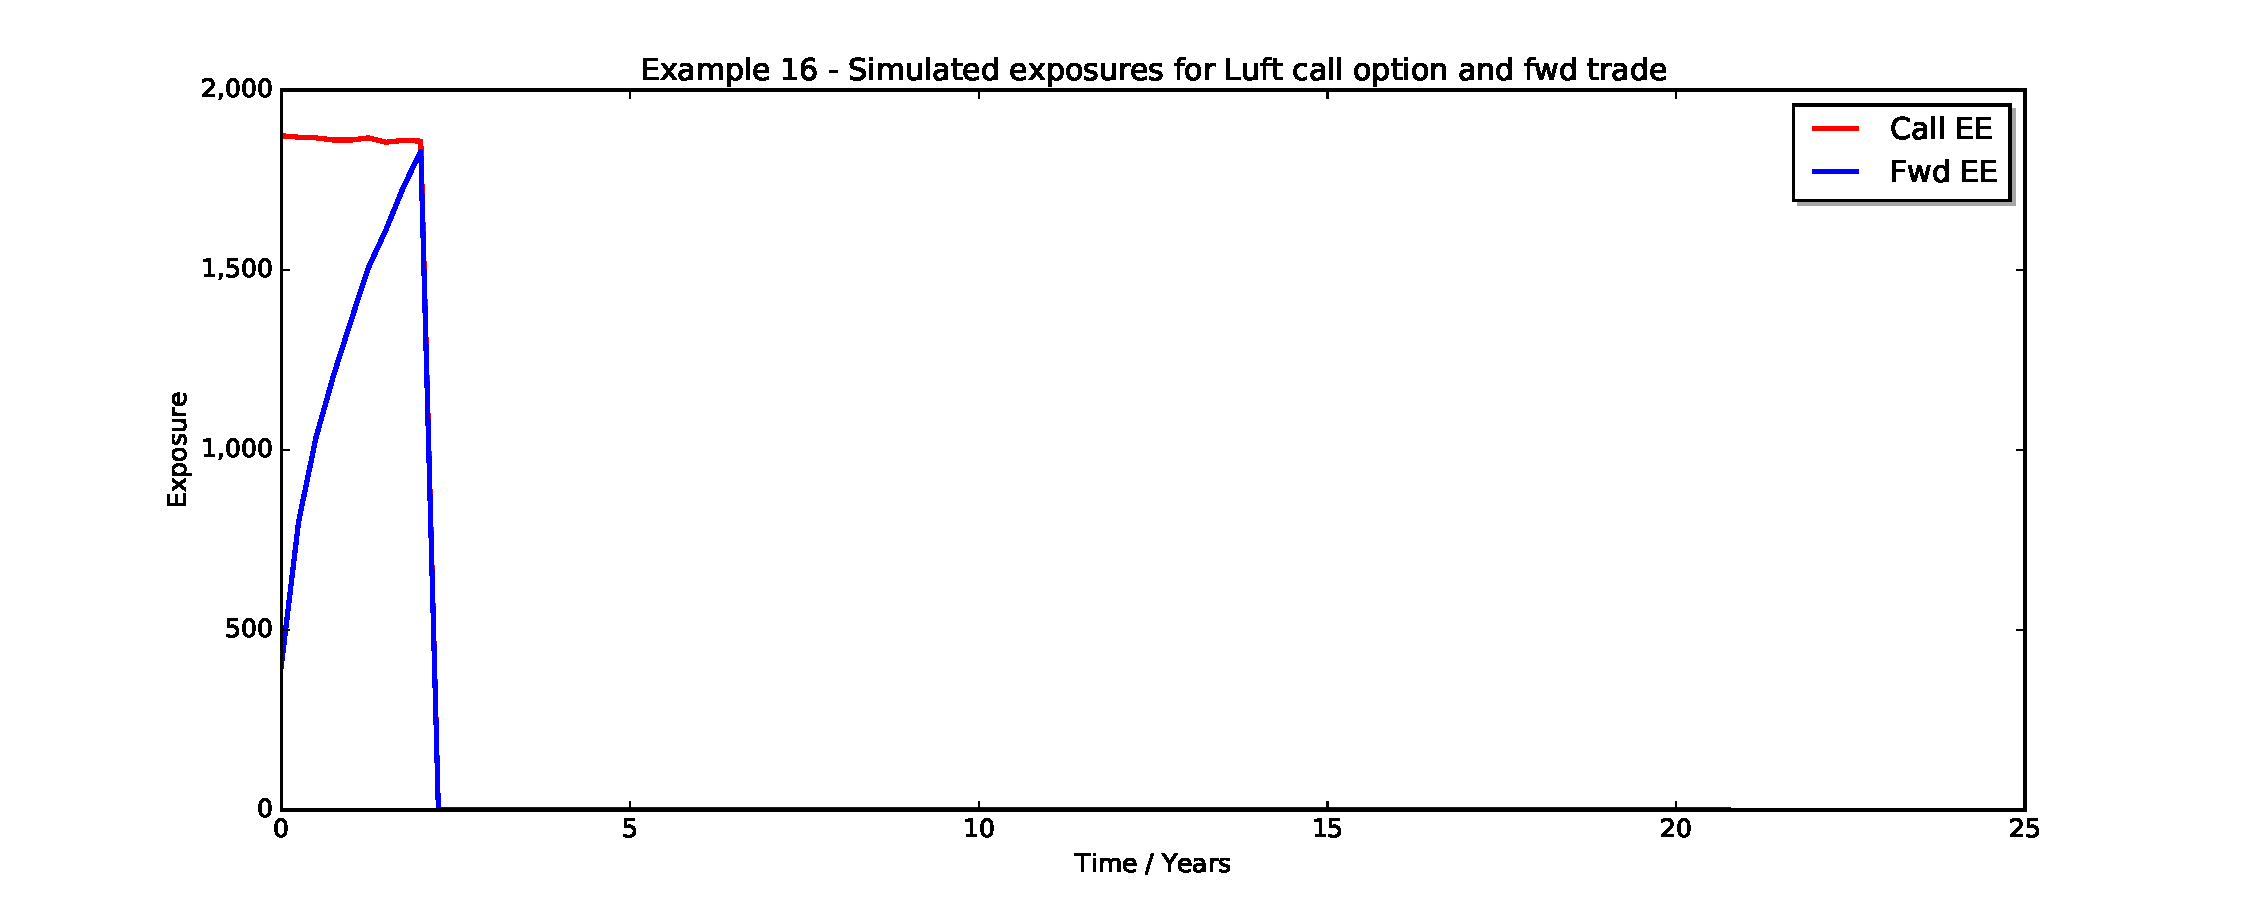
\includegraphics[scale=0.45]{examples/mpl_eq_call.pdf}
	\end{center}
	\caption{Equity (``Luft'') call option and OTC forward exposure evolution, maturity in approximately 2.5 years. 
	Simulation with 
	10000 paths and quarterly time steps.}
	\label{fig_eq_call}
\end{figure}

%--------------------------------------------------------
\subsection{Inflation Swap Exposure under Dodgson-Kainth}% Example 17
\label{example:17}
%--------------------------------------------------------

The example portfolio in folder {\tt Examples/Example\_17} contains two CPI Swaps and one Year-on-Year Inflation Swap.
The terms of the three trades are as follows:

\begin{itemize}
\item CPI Swap 1: Exchanges on 2036-02-05 a fixed amount of 20m GBP for a 10m GBP notional inflated with UKRPI with base CPI 210
\item CPI Swap 2: Notional 10m GBP, maturity 2021-07-18, exchanging GBP Libor for GBP Libor 6M vs. $2\%$ x CPI-Factor (Act/Act), inflated with index UKRPI with base CPI 210
\item YOY Swap: Notional 10m EUR, maturity 2021-02-05, exchanging fixed coupons for EUHICPXT year-on-year inflation coupons
\item YOY Swap with capped/floored YOY leg: Notional 10m EUR, maturity 2021-02-05, exchanging fixed coupons for EUHICPXT year-on-year inflation coupons, YOY leg capped with 0.03 and floored with 0.005
\item YOY Swap with scheduled capped/floored YOY leg: Notional 10m EUR, maturity 2021-02-05, exchanging fixed coupons for EUHICPXT year-on-year inflation coupons, YOY leg capped with cap schedule and floored with floor schedule
\end{itemize}

The example generates cash flows, NPVs, exposure evolutions, XVAs, as well as two exposure graphs for CPI Swap 1 respectively the YOY Swap. For the YOY Swap and the both YOY Swaps with capped/floored YOY leg, the example generates their cash flows, NPVs, exposure evolutions, XVAs and sensitivities. Figure \ref{fig_cpi_swap} shows the CPI Swap exposure evolution.

\begin{figure}[h!]
	\begin{center}
		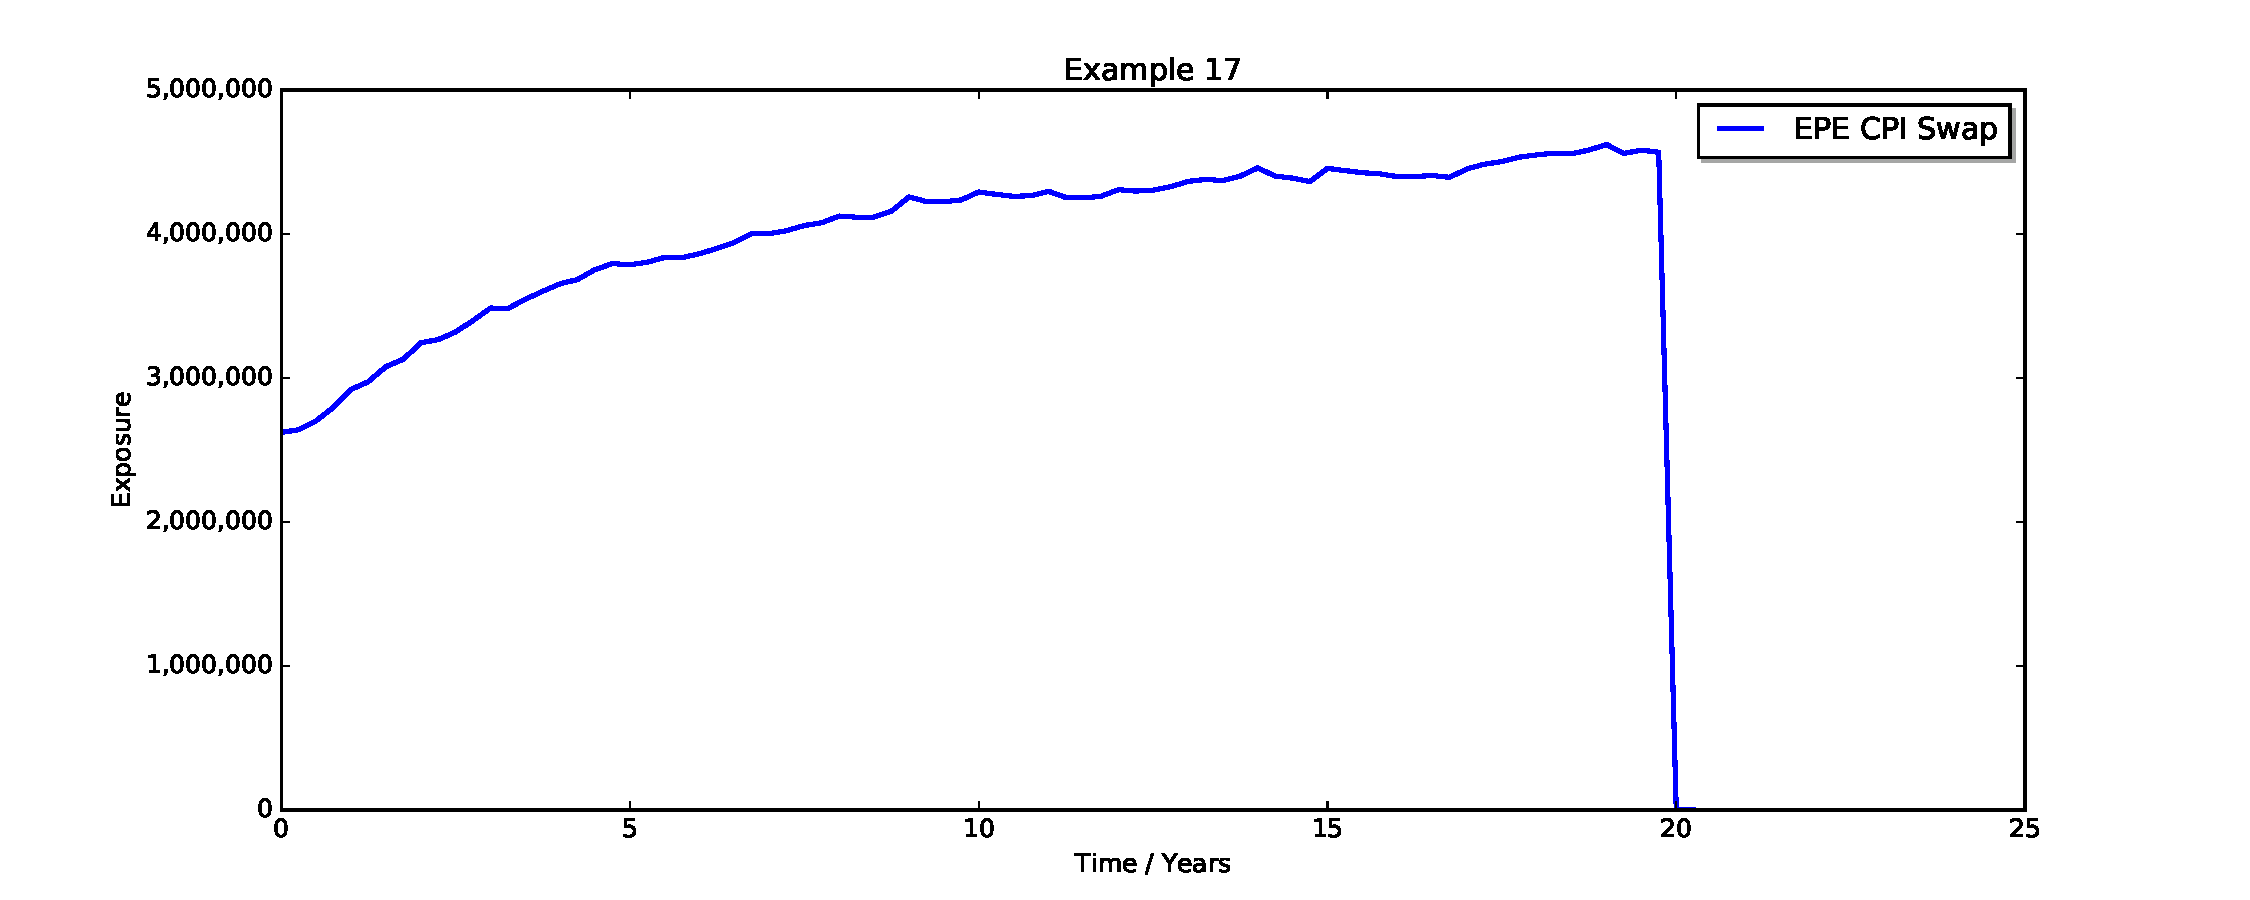
\includegraphics[scale=0.45]{examples/mpl_cpi_swap.pdf}
	\end{center}
	\caption{CPI Swap 1 exposure evolution. Simulation with 1000 paths and quarterly time steps.}
	\label{fig_cpi_swap}
\end{figure}

Figure \ref{fig_yoy_swap} shows the evolution of the 5Y maturity Year-on-Year inflation swap for comparison. Note that the inflation simulation model (Dodgson-Kainth, see \cite{methods}) yields the evolution of inflation indices and inflation zero bonds which allows spanning future inflation zero curves and the pricing of CPI swaps. To price Year-on-Year inflation Swaps under future scenarios, we imply Year-on-Year inflation curves from zero inflation curves\footnote{Currently we discard the required (small) convexity adjustment. This will be supplemented in a subsequent release.}. Note that for pricing Year-on-Year Swaps as of today we use a separate inflation curve bootstrapped from quoted Year-on-Year inflation Swaps.
 
\begin{figure}[h!]
	\begin{center}
		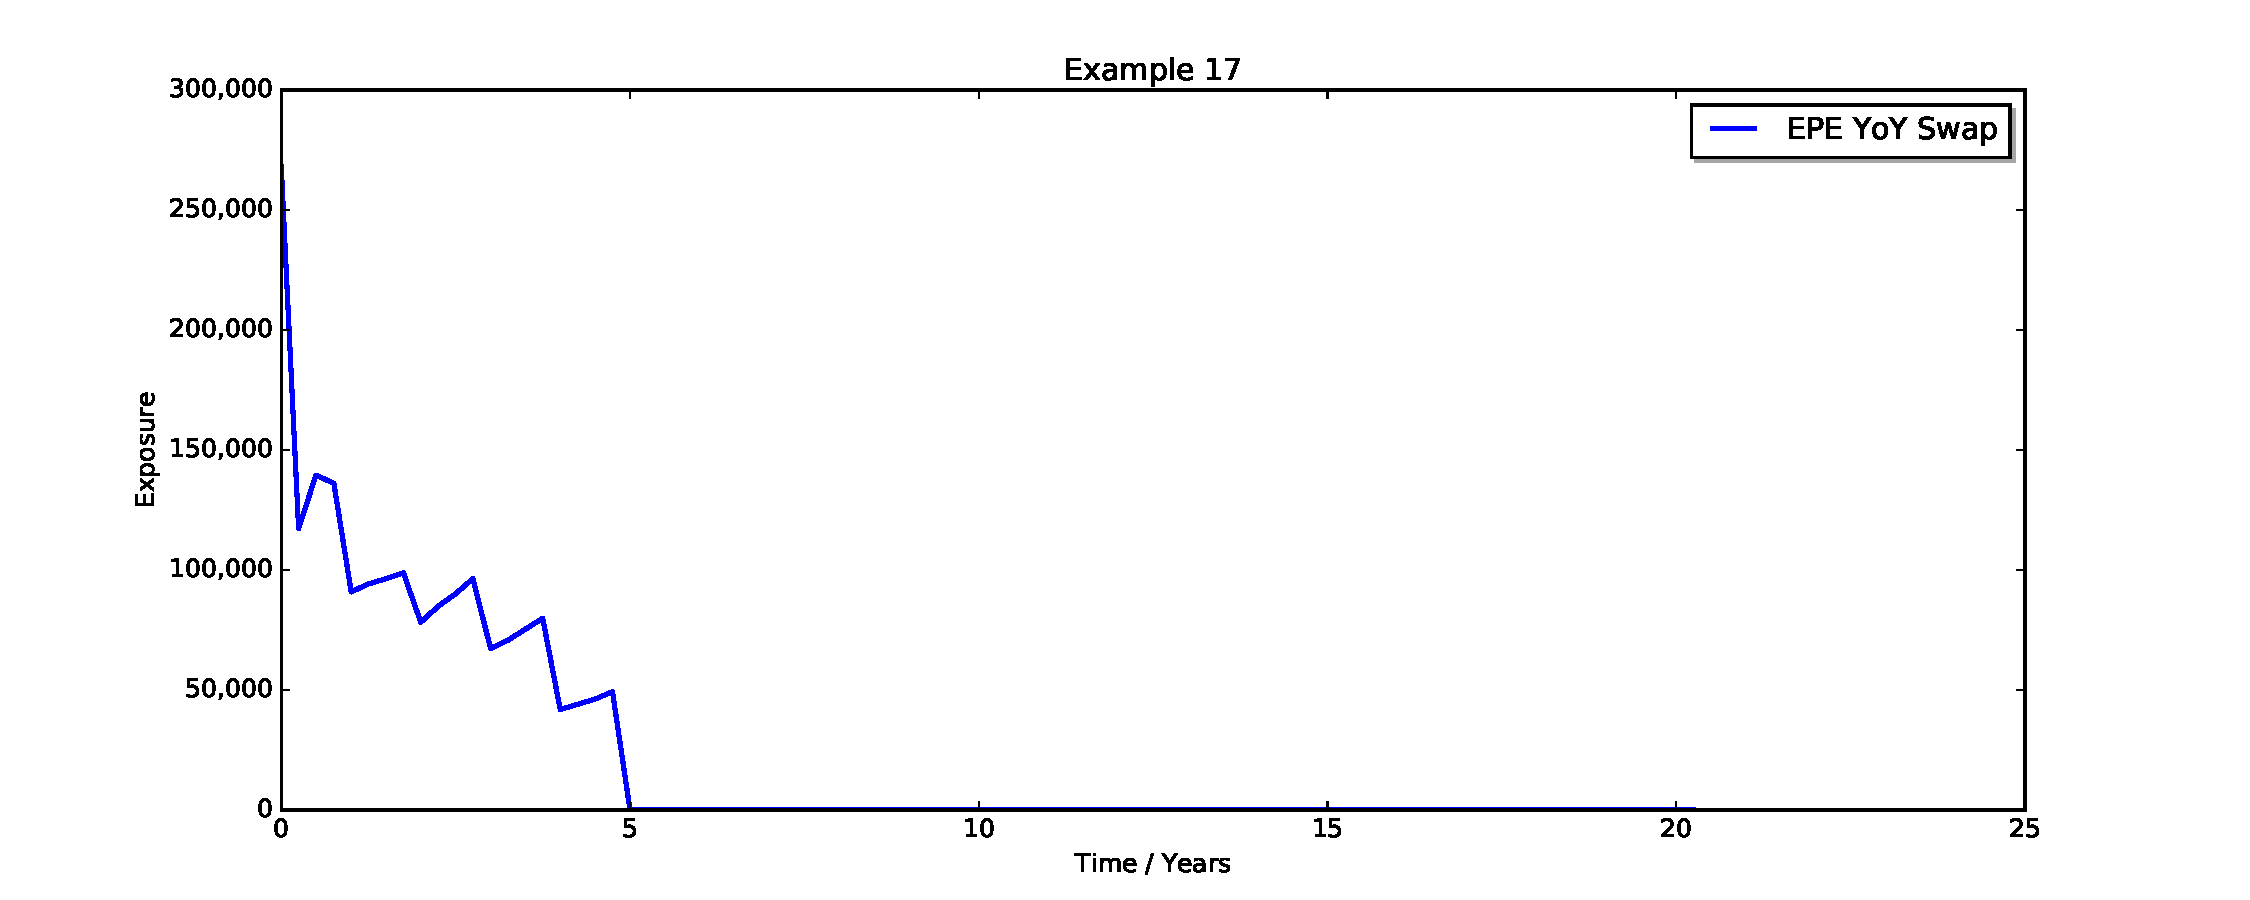
\includegraphics[scale=0.45]{examples/mpl_yoy_swap.pdf}
	\end{center}
	\caption{Year-on-Year Inflation Swap exposure evolution. Simulation with 1000 paths and quarterly time steps.}
	\label{fig_yoy_swap}
\end{figure}

%--------------------------------------------------------
\subsection{Bonds and Amortisation Structures}% Example 18
%--------------------------------------------------------

The example in folder {\tt Examples/Example\_18} computes NPVs and cash flow projections for a vanilla bond portfolio
consisting of a range of bond products, in particular demonstrating amortisation features. Also, pricing using a benchmark bond price curve (bond definitions in referencedata.xml) is demonstrated:
\begin{itemize}
\item fixed rate bond
\item floating rate bond linked to Euribor 6M
\item bond switching from fixed to floating
\item bond with 'fixed amount' amortisation
\item bond with percentage amortisation relative to the initial notional
\item bond with percentage amortisation relative to the previous notional
\item bond with fixed annuity amortisation
\item bond with floating annuity amortisation (this example needs QuantLib 1.10 or higher to work, in particular the amount() method in the Coupon class needs to be virtual)
\item bond with fixed amount amortisation followed by percentage amortisation relative to previous notional
\item fixed rate bond using a benchmark bond price curve instead of the benchmark yield curve
\end{itemize}

After running the example, the results of the computation can be found in the output files {\tt npv.csv} and {\tt
  flows.csv}, respectively.

\medskip
Note that the amortisation features used here are linked to the LegData structure, hence not limited to the Bond instrument, see \cite{products}. %section \ref{ss:amortisationdata}.

%--------------------------------------------------------
\subsection{Swaption Pricing with Smile}% Example 19
%--------------------------------------------------------

This example in folder {\tt Examples/Example\_19} demonstrates European Swaption pricing with and without smile. Calling

\medskip
\centerline{\tt python run.py}

\medskip
will launch two ORE runs using config files {\tt ore\_flat.xml} and {\tt ore\_smile.xml}, respectively. The only difference in these is referencing alternative market configurations {\tt todaymarket\_flat.xml} and {\tt todaysmarket\_smile.xml} using an ATM Swaption volatility matrix and a Swaption cube, respectively. NPV results are written to {\tt npv\_flat.cvs} and {\tt npv\_smile.csv}.

%--------------------------------------------------------
\subsection{Credit Default Swap Pricing}% Example 20
%--------------------------------------------------------

This example in folder {\tt Examples/Example\_20} demonstrates Credit Default Swap pricing via ORE. Calling

\medskip
\centerline{\tt python run.py}

\medskip
will launch a single ORE run to process a single name CDS example and to generate NPV and cash flows in the usual result files. 

\medskip
CDS can be included in sensitivity analysis and stress testing. Exposure simulation for credit derivatives will follow in the next ORE release.

%--------------------------------------------------------
\subsection{CMS and CMS Cap/Floor Pricing}% Example 21
%--------------------------------------------------------

This example in folder {\tt Examples/Example\_21} demonstrates the pricing of CMS and CMS Cap/Floor using a portfolio consisting of a CMS Swap (CMS leg vs. fixed leg) and a CMS Cap. Calling

\medskip
\centerline{\tt python run.py}

\medskip
will launch a single ORE run to process the portfolio and generate NPV and cash flows in the usual result files. 

\medskip
CMS structures can be included in sensitivity analysis, stress testing and exposure simulation. 

%--------------------------------------------------------
\subsection{Option Sensitivity Analysis with Smile}% Example 22
%--------------------------------------------------------

The example in folder {\tt Examples/Example\_22} demonstrates the current state of sensitivity calculation for European options where the volatility surface has a smile. 

\medskip
The portfolio used in this example consists of
\begin{itemize}
	\item an equity call option denominated in USD (``SP5'')
	\item an equity put option denominated in USD (``SP5'')
	\item a receiver swaption in EUR
	\item an FX call option on EUR/USD
\end{itemize}

\medskip
Refer to \cite{methods} for the current status of sensitivity implementation with smile. In this example the setup is as follows
\begin{itemize}
\item today's market is configured with volatility smile for all three products above
\item simulation market has two configurations, to simulate ``ATM only'' or the ``full surface''; ``ATM only'' means that only ATM volatilities are to be simulated and shifts to ATM vols are propagated to the respective smile section;
\item the sensitivity analysis has two corresponding configurations as well, ``ATM only'' and ``full surface''; note that the ``full surface'' configuration leads to explicit sensitivities by strike only in the case of Swaption volatilities, for FX and Equity volatilities only ATM sensitivity can be specified at the moment and sensitivity output is currently aggregated to the ATM bucket (to be extended in subsequent releases).
\end{itemize}

The respective output files end with ``{\tt\_fullSurface.csv}'' respectively ``{\tt\_atmOnly.csv}''.

%ORE supports two methods of simulating equity volatility smile. The first method simulates the entire surface using specific moneyness levels configured in simulation.xml. The second method simulates only the ATM equity volatilities, the other strikes are shifted relative to this new ATM using the $t_{0}$ smile.  This example compares both methods using the same sensitivity configuration as in {\tt Examples/Example\_15}. For the first method {\tt simulation\_fullSurface.xml} is used and all output files are appended with ``\_fullSurface'', for the second method {\tt simulation\_atmOnly.xml} is used and all output files are appended with ``\_atmOnly''.


%--------------------------------------------------------
\subsection{FRA and Average OIS Exposure}% Example 23
%--------------------------------------------------------

This example in folder {\tt Examples/Example\_23} demonstrates pricing, cash flow projection and exposure simulation for two additional products
\begin{itemize}
\item Forward Rate Agreements
\item Averaging Overnight Index Swaps
\end{itemize}
using a minimal portfolio of four trades, one FRA and three OIS. The essential results are in {\tt npv.csv}, {\tt flows.csv} and 
four {\tt exposure\_trade\_*.csv} files.

%--------------------------------------------------------
\subsection{Commodity Derivatives, Pricing, Sensitivity, Exposure}% Example 24
\label{example:24}
%--------------------------------------------------------

Calling

\medskip
\centerline{\tt python run.py}

\medskip
in folder {\tt Examples/Example\_24} will launch two ORE runs. The first one determined by {\tt ore.xml} demonstrates pricing and sensitivity analysis for
\begin{itemize}
\item Commodity Forwards
\item European Commodity Options
\end{itemize}
using a minimal portfolio of four forwards and two options referencing WTI and Gold. 
The essential results are in {\tt npv.csv} and {\tt sensitivity.csv}.

The second run determined by {\tt ore\_wti.xml} demonstrates Commodity exposure simulation for a portfolio including a
\begin{itemize}
\item Commodity Forward
\item Commodity Swap
\item European Commodity Option
\item Commodity Average Price Option
\item Commodity Swaption
\end{itemize}
with the usual results, exposure reports and graphs. 

%--------------------------------------------------------
\subsection{CMS Spread with (Digital) Cap/Floor}% Example 25
\label{example:25}
%--------------------------------------------------------

The example in folder {\tt Examples/Example\_25}  demonstrates pricing, sensitivity analysis 
and exposure simulation for 
\begin{itemize}
\item Capped/Floored CMS Spreads
\item CMS Spreads with Digital Caps/Floors
\end{itemize}

The example can be run with

\medskip
\centerline{\tt python run.py}

\medskip
and results are in {\tt npv.csv}, {\tt sensitivity.csv}, {\tt exposure\_*.csv} 
and the exposure graphs in {\tt mpl\_cmsspread.pdf}.

%--------------------------------------------------------
\subsection{Bootstrap Consistency}% Example 26
%--------------------------------------------------------

The example in folder {\tt Examples/Example\_26} confirms that bootstrapped curves 
correctly reprice the bootstrap instruments (FRAs, Interest Rate Swaps, FX Forwards, Cross
Currency Basis Swaps) using three pricing setups with
\begin{itemize}
\item EUR collateral discounting (configuration xois\_eur)
\item USD collateral discounting (configuration xois\_usd)
\item in-currency OIS discounting (configuration collateral\_inccy)
\end{itemize}
all defined in {\tt Examples/Input/todaysmarket.xml}.

\medskip
The required portfolio files need to be generated from market data and conventions in
{\tt Examples/Input} and trade templates in 
{\tt Examples/Example\_26/Helpers}, calling

\medskip
\centerline{\tt python TradeGenerator.py}

\medskip
This will place three portfolio files {\tt *\_portfolio.xml} in the input folder.
Thereafter, the three consistency checks can be run calling

\medskip
\centerline{\tt python run.py}

\medskip
Results are in three files {\tt *\_npv.csv} and should show zero NPVs for all benchmark instruments.

%--------------------------------------------------------
\subsection{BMA Basis Swap}% Example 27
\label{example:27}
%--------------------------------------------------------

The example in folder {\tt Examples/Example\_27} demonstrates pricing 
and sensitivity analysis for a series of USD Libor 3M vs. Averaged BMA (SIFMA) 
Swaps that correspond to the instruments used to bootstrap the BMA curve. 

The example can be run with

\medskip
\centerline{\tt python run.py}

\medskip
and results are in {\tt npv.csv} and {\tt sensitivity.csv}.

%--------------------------------------------------------
\subsection{Discount Ratio Curves}% Example 28
\label{example:28}
%--------------------------------------------------------

The example in folder {\tt Examples/Example\_28} shows how to use a yield curve 
built from a DiscountRatio segment. 
In particular, it builds a GBP collateralized in EUR discount curve by referencing 
three other discount curves:
\begin{itemize}
\item a GBP collateralised in USD curve
\item a EUR collateralised in USD curve
\item a EUR OIS curve i.e. a EUR collateralised in EUR curve
\end{itemize}

The implicit assumption in building the curve this way is that EUR/GBP FX 
forwards collateralised in EUR have the same fair market rate as EUR/GBP 
FX forwards collateralised in USD. This assumption is illustrated in the 
example by the NPV of the two forward instruments in the portfolio returning 
exactly 0 under both discounting regimes i.e. under USD collateralization with 
direct curve building and under EUR collateralization with the discount ratio 
modified ``GBP-IN-EUR'' curve.

Also, in this example, an assumption is made that there are no direct GBP/EUR FX 
forward or cross currency quotes available which in general is false. The example 
s merely for illustration.

Both collateralizaton scenarios can be run calling {\tt python run.py}.

%--------------------------------------------------------
\subsection{Curve Building using Fixed vs. Float Cross Currency Helpers}% Example 29
\label{example:29}
%--------------------------------------------------------

The example in folder {\tt Examples/Example\_29} demonstrates using fixed vs. float 
cross currency swap helpers. In particular, it builds a TRY collateralised in USD 
discount curve using TRY annual fixed vs USD 3M Libor swap quotes.

The portfolio contains an at-market fixed vs. float cross currency swap that is 
included in the curve building. The NPV of this swap should be zero when the example is run,
using {\tt python run.py} or ``directly'' calling {\tt ore[.exe] ore.xml}.

%--------------------------------------------------------
\subsection{USD-Prime Curve Building via Prime-LIBOR Basis Swap}% Example 30
\label{example:30}
%--------------------------------------------------------

The example in folder {\tt Examples/Example\_30} demonstrates the implementation of the USD-Prime index in the ORE.
The USD-Prime yield curve is built from USD-Prime vs USD 3M Libor basis swap quotes.
The portfolio consists of two fair basis swaps (NPVs equal to 0):
\begin{itemize}
\item US Dollar Prime Rate vs 3 Month LIBOR
\item US Dollar 3 Month LIBOR vs Fed Funds + 0.027
\end{itemize}

In particular, it is confirmed that the bootstrapped curves USD-FedFunds and USD-Prime follow
the 3\% rule observed on the market: {\tt U.S. Prime Rate = (The Fed Funds Target Rate + 3\%)}.
(See \url{http://www.fedprimerate.com/}.)

Running ORE in directory {\tt Examples/Example\_30} with {\tt python run.py }
yields the USD-Prime curve in {\tt Examples/Example\_30/Output/curves.csv.}

%--------------------------------------------------------
\subsection{Exposure Simulation using a Close-Out Grid}% Example 31
\label{example:31}
%--------------------------------------------------------

In the previous examples we have used a ``lagged'' approach, described at the end of the collateral section in \cite{methods},
to take the Margin Period of Risk into account in exposure modelling. This used to have the disadvantage in ORE that we need
to use equally-spaced time grids with time steps that match the MPoR, e.g. 2W, out to final portfolio maturity. 

In this example we demonstrate an alternative approach supported by ORE since release 6. In this approach we use two nested grids: The (almost) arbitrary main simulation grid is used to compute ``default values'' which feed into the collateral balance $C(t)$ filtered by MTA and Threshold etc; an auxiliary ``close-out'' grid, offset from the main grid by the MPoR, is used to compute the delayed close-out values $V(t)$ associated with time default time $t$. The difference between $V(t)$ and $C(t)$ causes a residual exposure $[V(t)-C(t)]^+$ even if minimum transfer amounts and thresholds are zero.

The close-out date value can be computed in two ways in ORE
\begin{itemize}
\item as of default date, by just evolving the market from default date to close-out date
   (``sticky date''), or 
\item  as of close-out date, by evolving both valuation date and market over the 
   close-out period (``actual date''), i.e., the portfolio ages and cash flows might occur
   in the close-out period causing spikes in the evolution of exposures. 
\end{itemize}

We are reusing one case from Example 10 here, perfect CSA with zero threshold and
minimum transfer amount, so that the remaining exposure is solely due to the MPoR
effect. The portfolio consists of a single at-the-money Swap in GBP. 
The relevant configuration changes that trigger this modelling are in the Parameters section of {\tt simulation.xml} as shown in Listing \ref{lst:close_out_grid}

\begin{listing}[H]
\begin{minted}[fontsize=\footnotesize]{xml}
  <Parameters>
    <Grid> ... </Grid>
    <Calendar> ... </Calendar>
    <Sequence> ... </Sequence>
    <Scenario> ... </Scenario>
    <Seed> ... </Seed>
    <Samples> ... </Samples>
    <CloseOutLag> 2W </CloseOutLag>
    <MporMode> StickyDate </MporMode><!-- Alternative: ActualDate -->
  </Parameters>
\end{minted}
\caption{Close-out grid specification}
\label{lst:close_out_grid}
\end{listing}

and moreover in the XVA analytics section of {\tt ore\_mpor.xml} as shown in Listing \ref{lst:calctype_nolag}.

\begin{listing}[H]
\begin{minted}[fontsize=\footnotesize]{xml}
  <Analytic type="xva">
    ...
    <Parameter name="calculationType"> NoLag </Parameter>
    ...
  </Parameters>
\end{minted}
\caption{Close-out grid specification}
\label{lst:calctype_nolag}
\end{listing}

\begin{figure}[h!]
\begin{center}
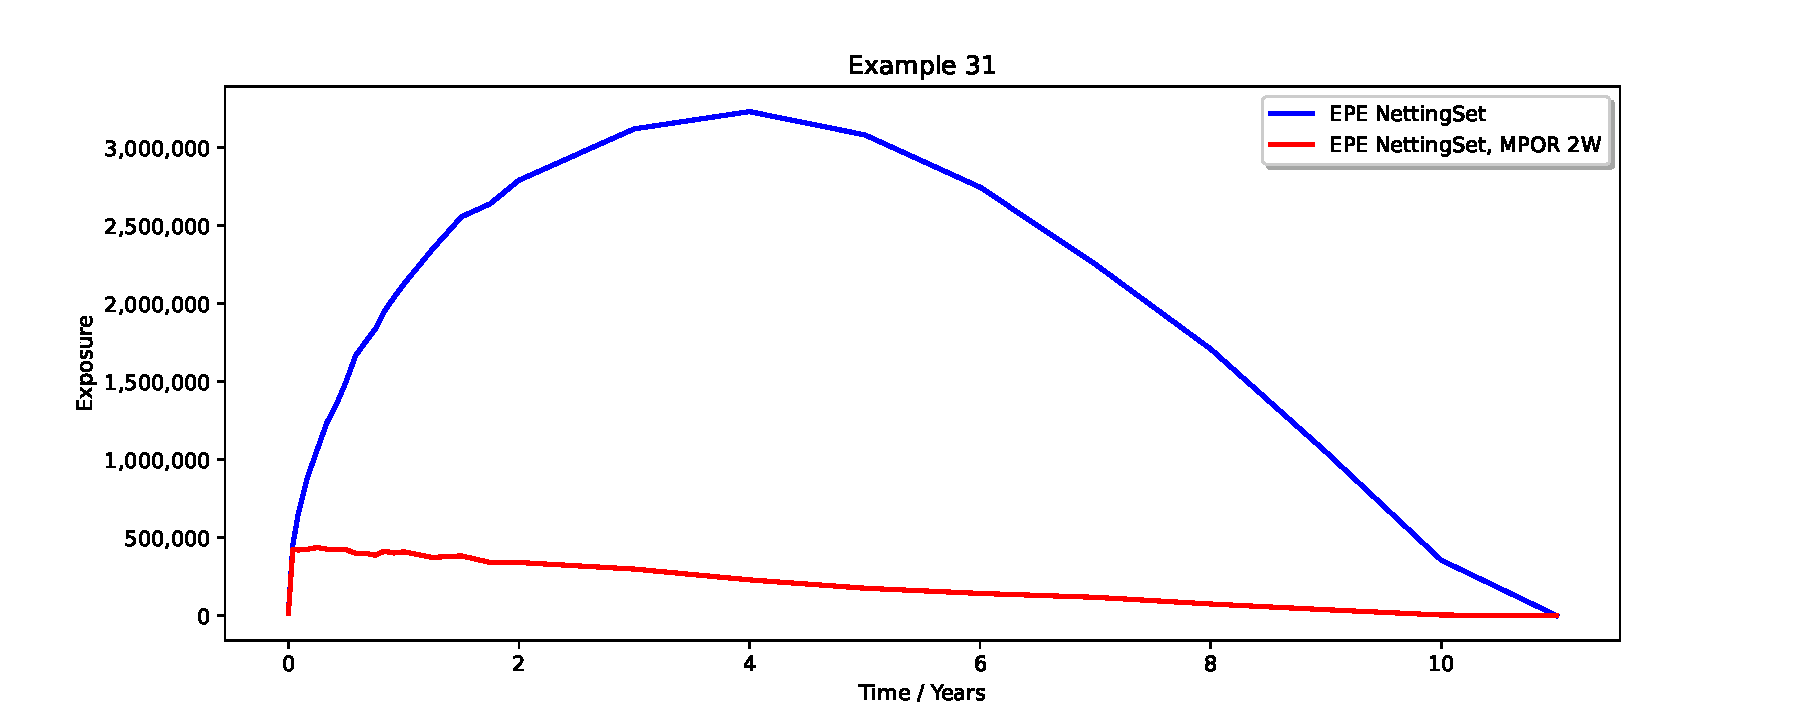
\includegraphics[scale=0.45]{examples/mpl_closeout_mpor_epe.pdf}
\end{center}
\caption{Uncollateralized Swap exposure vs exposure with Variation Margin, zero threshold and MTA.
  The simulation uses a variable grid with an auxiliary grid for closeout value calculation which is offset by the MPOR.}
\label{fig_31_a}
\end{figure}

\begin{figure}[h!]
\begin{center}
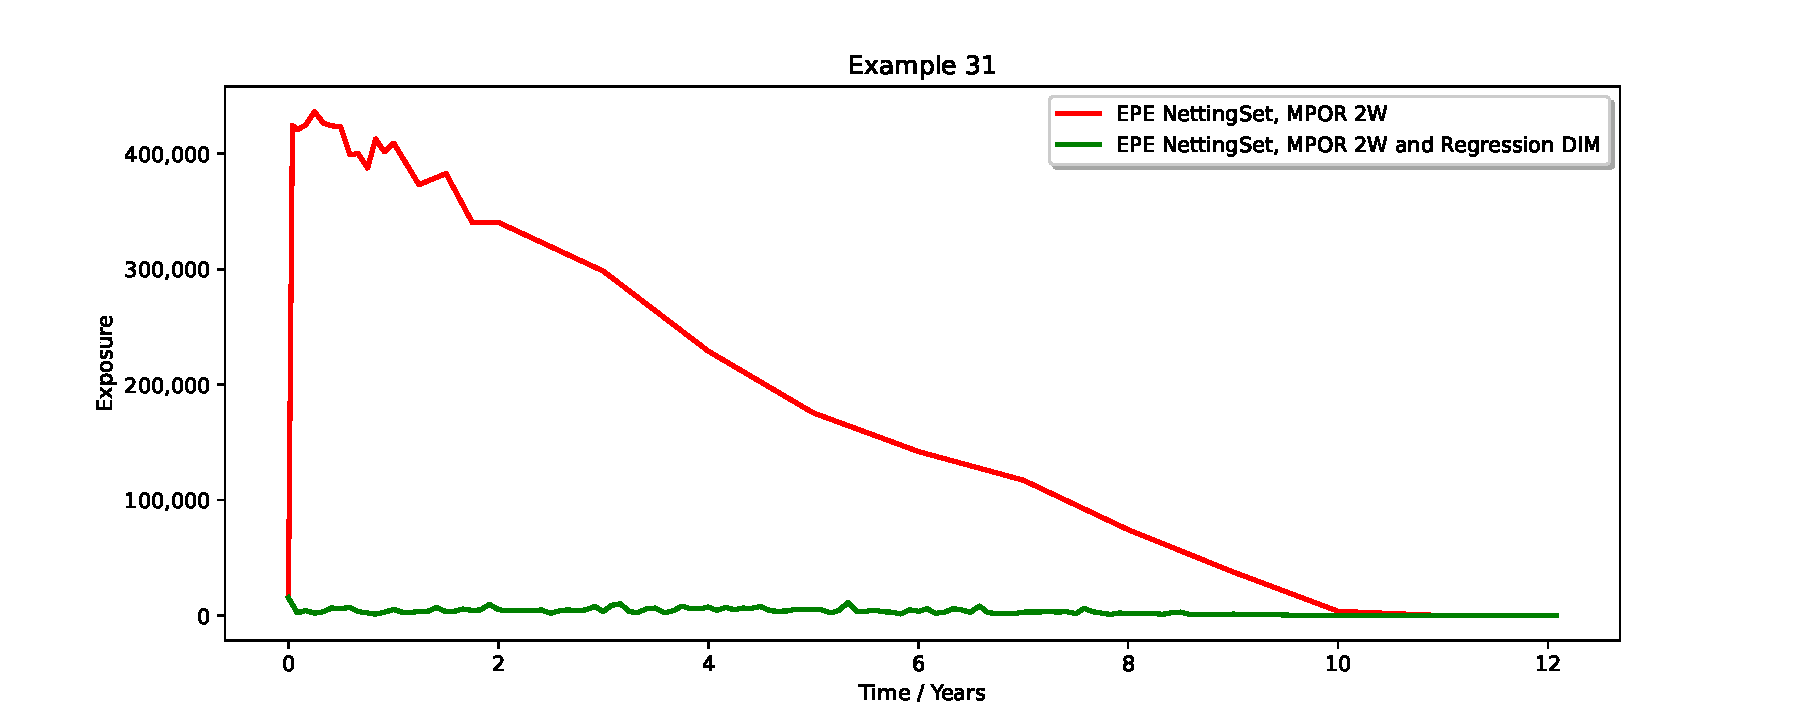
\includegraphics[scale=0.45]{examples/mpl_closeout_dim_epe.pdf}
\end{center}
\caption{Comparison of Swap exposure with VM only as above vs VM+IM using first-order regression.}
\label{fig_31_b}
\end{figure}

\begin{figure}[h!]
\begin{center}
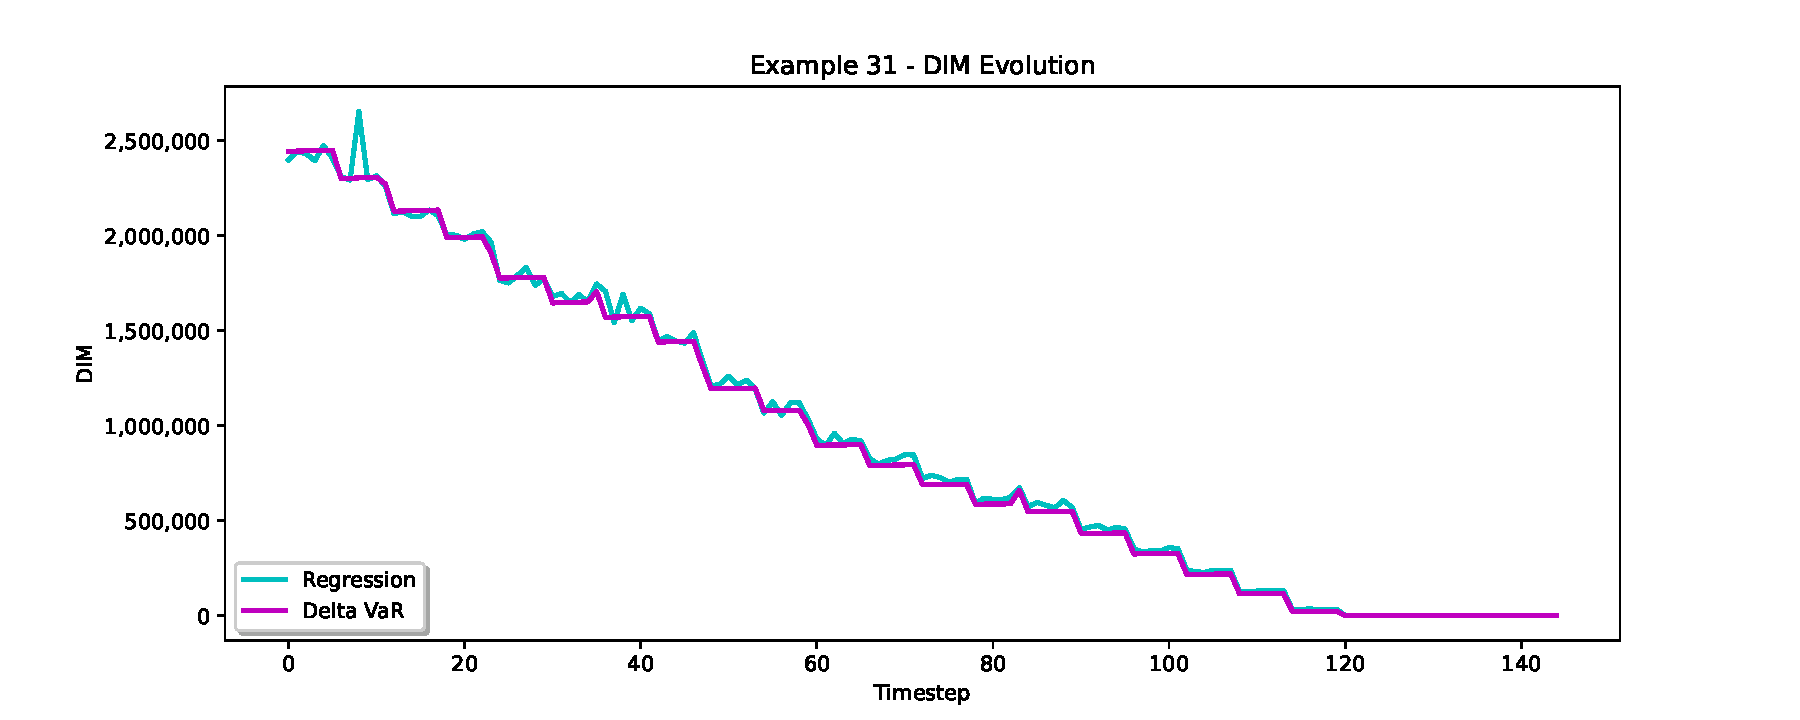
\includegraphics[scale=0.45]{examples/mpl_closeout_dim_evolution.pdf}
\end{center}
\caption{Evolution of expected IM from the regression model vs Delta VaR benchmark.}
\label{fig_31_c}
\end{figure}

Run as usual calling {\tt python run.py}. The resulting exposure graphs, with comparison of the uncollateralised to the collateralised
case (with Variation Margin only) is shown in figure \ref{fig_31_a}.

In figure \ref{fig_31_b} we have added Initial Margin based on ORE's regression model, and we compare the exposure with VM only to
the exposure with both VM and IM. This graph is also generated in this {\tt Example\_31}. Figure \ref{fig_31_c} shows the
related evolution of expected DIM, benchmarked against the Delta VaR DIM model, mentioned in {\tt Example\_13} and described in
\cite{methods}.

%--------------------------------------------------------------------
\subsection{Inflation Swap Exposure under Jarrow-Yildrim}% Example 32
\label{example:32}
%--------------------------------------------------------------------

The example here is similar to that in Section \ref{example:17} in that we are generating exposures for inflation swaps. The example in Section \ref{example:17} uses the Dodgson-Kainth model whereas this example uses the Jarrow-Yildrim model. The valuation date is 2 Nov 2020 and the portfolio contains four spot starting inflation swaps:

\begin{itemize}
\item trade\_01: 20Y standard UKRPI ZCIIS struck at the fair market rate of 3.1925\% giving an NPV of 0.0. 
\item trade\_02: 20Y standard EUHICPXT ZCIIS struck at the fair market rate of 1.16875\% giving an NPV of 0.0.
\item trade\_03: 20Y year on year EUHICPXT swap.
\item trade\_04: 20Y year on year UKRPI swap.
\end{itemize}

The example generates cash flows, NPVs, exposure evolutions and XVAs.

%--------------------------------------------------------------------
\subsection{CDS Exposure Simulation}% Example 33
\label{example:33}
%--------------------------------------------------------------------

The example in folder {\tt Examples/Example\_33} is the credit variant of the example in
\ref{sec:example1}. Running ORE in directory {\tt Examples/Example\_33} with

\medskip
\centerline{\tt python run.py } 
\medskip

yields the exposure evolution in 

\medskip
\centerline{\tt Examples/Example\_33/Output/*.pdf } 
\medskip

and shown in figure \ref{fig_33}. 
\begin{figure}[h!]
\begin{center}
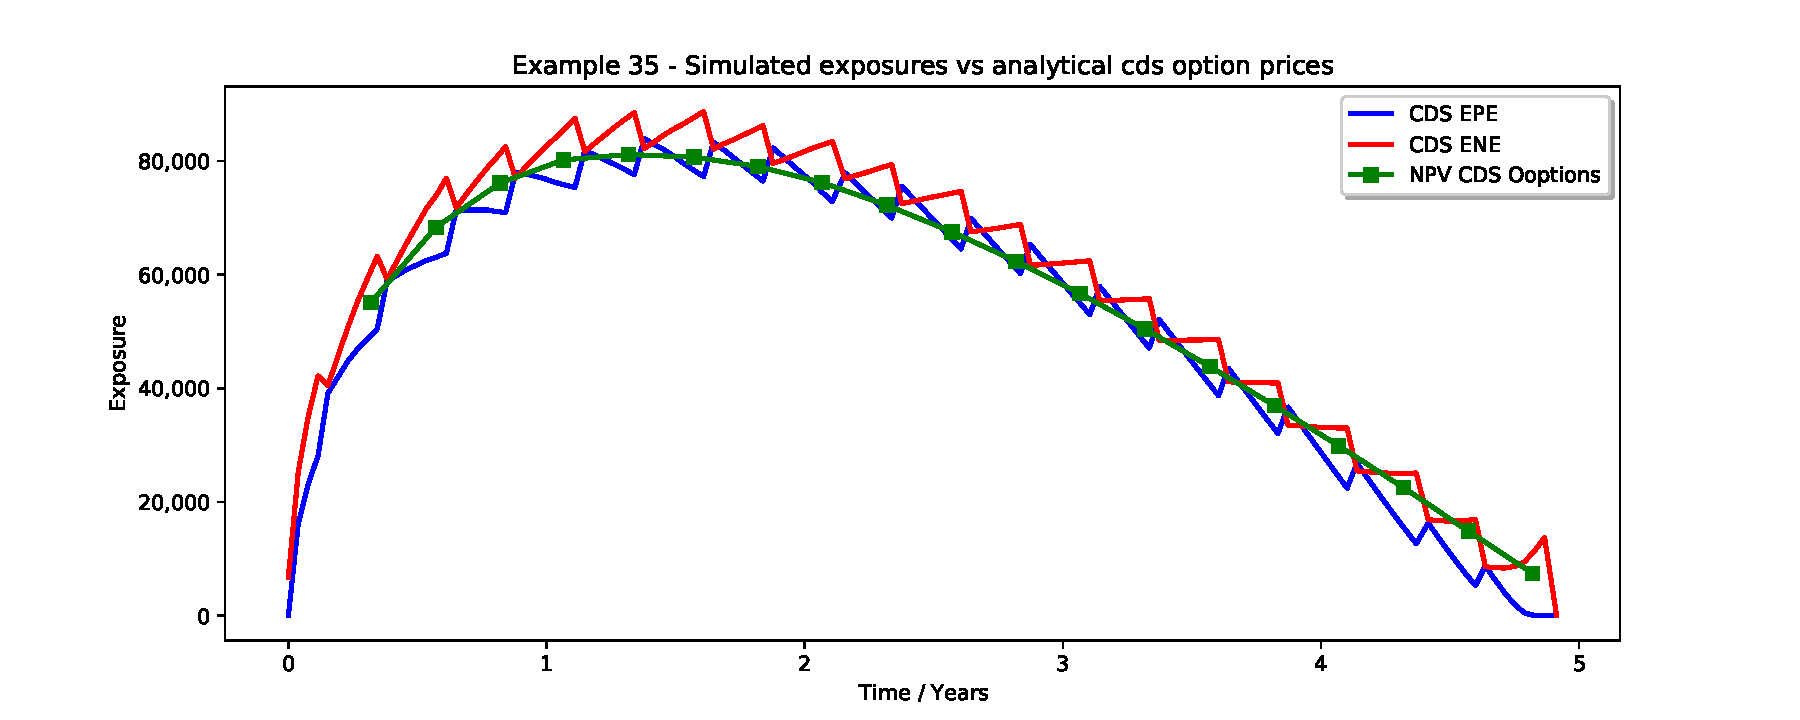
\includegraphics[scale=0.45]{examples/mpl_cds_33_2w_10k.pdf}
\end{center}
\caption{Credit Default Swap expected exposure in a flat market environment from both parties' perspectives. The symbols are CDS Option prices. The simulation was run with bi-weekly time steps and 10,000 Monte Carlo samples to demonstrate the convergence of EPE and ENE profiles. A similar
outcome can be obtained more quickly with 5,000 samples on a monthly time grid which is the default setting of Example\_33. }
\label{fig_33}
\end{figure}
Both CDS simulation and CDS Option pricing are run with calls to the ORE executable, essentially 

\medskip
\centerline{\tt ore[.exe] ore.xml} 

\centerline{\tt ore[.exe] ore\_cds\_option.xml} 
\medskip

which are wrapped into the script {\tt Examples/Example\_33/run.py} provided with the ORE release.

This example demonstrates credit simulation using the LGM model and the calculation of Wrong Way Risk due to credit
correlation between the underlying entity of the CDS and the counterparty of the CDS trade via dynamic credit.
Positive correlation between the two names weakens the protection of the CDS whilst
negative correlation strengthens the protection.

The following table lists the XVA result from the example at different levels of correlation.


\begin{table}[hbt]
\scriptsize
\begin{center}
\begin{tabular}{|r|l|r|r|r|r|}
\hline
Correlation & NettingSetId & CVA & DVA & FBA & FCA \\
\hline
-100\%  &  CPTY\_B  &  -2,638  &  2,906  &  486  &  -1,057 \\
 -90\%  &  CPTY\_B  &  -2,204  &  2,906  &  488  &  -1,053 \\
 -50\%  &  CPTY\_B  &    -485  &  2,906  &  493  &  -1,040 \\
 -40\%  &  CPTY\_B  &     -60  &  2,906  &  495  &  -1,037 \\
 -30\%  &  CPTY\_B  &     363  &  2,906  &  496  &  -1,033 \\
 -20\%  &  CPTY\_B  &     784  &  2,906  &  498  &  -1,030 \\
 -10\%  &  CPTY\_B  &   1,204  &  2,906  &  500  &  -1,027 \\
   0\%  &  CPTY\_B  &   1,621  &  2,906  &  501  &  -1,023 \\
  10\%  &  CPTY\_B  &   2,036  &  2,906  &  503  &  -1,020 \\
  20\%  &  CPTY\_B  &   2,450  &  2,906  &  504  &  -1,017 \\
  30\%  &  CPTY\_B  &   2,861  &  2,906  &  506  &  -1,013 \\
  40\%  &  CPTY\_B  &   3,271  &  2,906  &  507  &  -1,010 \\
  50\%  &  CPTY\_B  &   3,679  &  2,906  &  509  &  -1,017 \\
  90\%  &  CPTY\_B  &   5,290  &  2,906  &  515  &    -994 \\
 100\%  &  CPTY\_B  &   5,689  &  2,906  &  517  &    -991 \\
\hline
\end{tabular}
\caption{CDS XVA results with LGM model}
\end{center}
\end{table}

%--------------------------------------------------------------------
\subsection{Wrong Way Risk}% Example 34
\label{example:34}
%--------------------------------------------------------------------

The example in folder {\tt Examples/Example\_34} is an extension of the example in
\ref{sec:example1} with dynamic credit and IR-CR correlation. As we are paying
float, negative correlation implies that we pay more when the counterparty's credit
worsens, leading to a surge of CVA.

The following table lists the XVA result from the example at different levels of correlation.

\begin{table}[hbt]
\scriptsize
\begin{center}
\begin{tabular}{|r|l|r|r|r|r|}
\hline
Correlation & NettingSetId & CVA & DVA & FBA & FCA \\
\hline
 -30\%  &  CPTY\_A  & 105,146  &  68,061  &  31,519  &  -4,127 \\
 -20\%  &  CPTY\_A  &  88,442  &  68,061  &  30,976  &  -4,219 \\
 -10\%  &  CPTY\_A  &  71,059  &  68,061  &  30,439  &  -4,314 \\
   0\%  &  CPTY\_A  &  52,983  &  68,061  &  29,909  &  -4,411 \\
  10\%  &  CPTY\_A  &  34,199  &  68,061  &  29,386  &  -4,511 \\
  20\%  &  CPTY\_A  &  14,691  &  68,061  &  28,869  &  -4,614 \\
  30\%  &  CPTY\_A  &  -5,554  &  68,061  &  28,360  &  -4,719 \\
\hline
\end{tabular}
\caption{IR Swap XVA results with LGM model}
\end{center}
\end{table}

%--------------------------------------------------------------------
\subsection{Flip View}% Example 35
\label{example:35}
%--------------------------------------------------------------------

The example in folder {\tt Examples/Example\_35} demonstrates how ORE can be used to quickly switch perspectives in XVA calculations with minimal changes in the {\tt ore.xml} file only. In particular it does not involve manipulating the portfolio input or the netting set.

%--------------------------------------------------------------------
\subsection{Choice of Measure}% Example 36
\label{example:36}
%--------------------------------------------------------------------

The example in folder {\tt Examples/Example\_36} illustrates the effect of measure changes on simulated expected and peak exposures. For that purpose we reuse Example 1 (un-collateralized vanilla swap exposure) and run the simulation three times with different risk-neutral measures,
\begin{itemize}
\item in the LGM measure as in Example 1 (note {\tt <Measure>LGM</Measure>} in {\tt simulation\_lgm.xml}, this is the default also if the Measure tag is omitted)  
\item in the more common Bank Account measure (note {\tt <Measure>BA</Measure>} in {\tt simulation\_ba.xml})  
\item in the T-Forward measure with horizon T=20 at the Swap maturity (note {\tt <Measure>LGM</Measure>}  and {\tt <ShiftHorizon>20.0</ShiftHorizon>} in {\tt simulation\_fwd.xml})
\end{itemize}

The results are summarized in the exposure evolution graphs in figure \ref{fig:36}. As expected, the expected exposures evolutions match across measures, as these are expected discounted NPVs and hence measure independent.
However, peak exposures are dependent on the measure choice as confirmed graphically here. Many more measures are accessible with ORE, by way of varying the T-Forward horizon which was chosen arbitrarily here to match the Swap's maturity.

\begin{figure}[h!]
\begin{center}
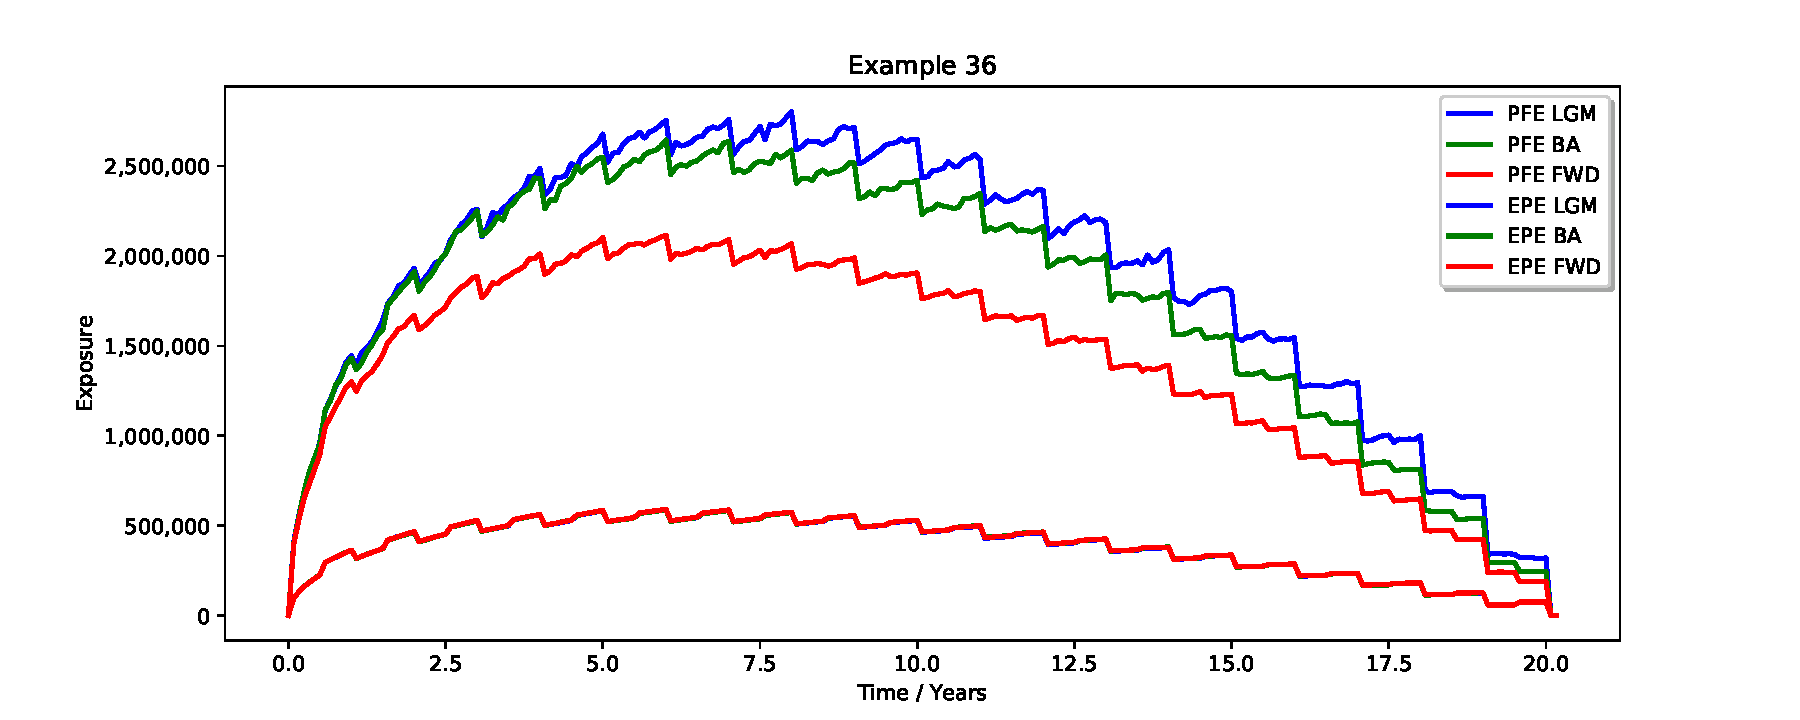
\includegraphics[scale=0.45]{examples/mpl_exposures_measures.pdf}
\end{center}
\caption{Evolution of expected exposures (EPE) and peak exposures (PFE at the 95\% quantile) in three measures, LGM, Bank Account, T-Forward with T=20, with 10k Monte Carlo samples.}
\label{fig:36}
\end{figure}

%--------------------------------------------------------------------
\subsection{Multifactor Hull-White Scenario Generation}% Example 37
\label{example:37}
%--------------------------------------------------------------------

The example in folder {\tt Examples/Example\_37} illustrates the scenario generation under a Hull-White multifactor
model. The model is driven by two independent Brownian motions and has four states. The diffusion matrix sigma is
therefore 2 x 4. The reversion matrix is a 4 x 4 diagonal matrix and entered as an array. Both diffusion and reversion
are constant in time. Their values are not calibrated to the option market, but hardcoded in simulation.xml.

The values for the diffusion and reversion matrices were fitted to the first two principal components of a
(hypothetical) analyis of absolute rate curve movements. These input principal components can be found in
inputeigenvectors.csv in the input folder. The tenor is given in years, and the two components are given as column
vectors, see table \ref{tab:ex37_1}.

\begin{table}[hbt]
\begin{center}
\begin{tabular}{r|r|r}
tenor & eigenvector 1  & eigenvector 2   \\
\hline      
1     & 0.353553390593 & -0.537955502871 \\
2     & 0.353553390593 & -0.374924478795 \\
3     & 0.353553390593 & -0.252916811525 \\
5     & 0.353553390593 & -0.087587539893 \\
10    & 0.353553390593 & 0.12267800393   \\
15    & 0.353553390593 & 0.240659435416  \\
20    & 0.353553390593 & 0.339148675322  \\
30    & 0.353553390593 & 0.552478951238
\end{tabular}
\caption{Input principal components}
\label{tab:ex37_1}
\end{center}
\end{table}

The first eigenvector represent perfectly parallel movements. The second eigenvector represent a rotation around the 7y
point of the curve. Furthermore we prescribe an annual volatility of 0.0070 for the first components and 0.0030 for the
second one. The values can be compared to normal (bp) volatilities.

We follow \cite{Andersen_Piterbarg_2010} chapter 12.1.5 ``Multi-Factor Statistical Gaussian Model'' to calibrate the
diffusion and reversion matrices to the prescribed components and volatilities. We do not detail the procedure here and
refer the interested reader to the given reference.

The example generates a single monte carlo path with 5000 daily steps and outputs the generated scenarios in
scenariodump.csv. The python script pca.py performs a principal component analysis on this output. The model implied
eigenvalues are given in table \ref{tab:ex37_2}.

\begin{table}[hbt]
\begin{center}
\begin{tabular}{r|r}
number & value                  \\
\hline      
1      & 4.9144936649319346e-05 \\
2      & 8.846877641067412e-06  \\
3      & 5.82566039467854e-10   \\
4      & 2.1298948225571415e-10 \\
5      & 9.254913949332787e-11  \\
6      & 1.0861256211767673e-11 \\
7      & 8.478795662698618e-14  \\
8      & 9.74468069377584e-13   \\
\end{tabular}
\caption{Input principal components}
\label{tab:ex37_2}
\end{center}
\end{table}

Only the first two values are relevant, the following are all close to zero. The square root of the first two
eigenvalues is given in table \ref{tab:ex37_3}.

\begin{table}[hbt]
\begin{center}
\begin{tabular}{r|r}
number & sqrt(value)                \\
\hline      
1      & 0.007010344973631422       \\
2      & 0.0029743701250966414      \\
\end{tabular}
\caption{Input principal components}
\label{tab:ex37_3}
\end{center}
\end{table}

matching the prescribed input values of 0.0070 and 0.0030 quite well. The correpsonding eigenvectors are given in etable
\ref{tab:ex37_4}.

\begin{table}[hbt]
\begin{center}
\begin{tabular}{r|r|r}
tenor & eigenvector 1       & eigenvector 2       \\
\hline      
1     & 0.34688826736335926 & 0.5441204725042812  \\
2     & 0.3489303472083185  & 0.380259707350115   \\
3     & 0.350362134519783   & 0.2581408080614405  \\
5     & 0.3523983915961889  & 0.09230899007104967 \\
10    & 0.3550169593982022  & -0.11856777284904292\\
15    & 0.35647835947136625 & -0.23676104168229614\\
20    & 0.3577146190751303  & -0.3354486339442275 \\
30    & 0.36042236352102563 & -0.549124709243042  \\
\end{tabular}
\caption{Input principal components}
\label{tab:ex37_4}
\end{center}
\end{table}

again matching the input principal components quite well. The second eigenvector is the negative of the input vector
here (the principal compoennt analysis can not distinguish these of course).

The example also produces a plot comparing the input eigenvectors and the model implied eigenvectors as shown in figure \ref{fig:ex37}.

\begin{figure}[h!]
\begin{center}
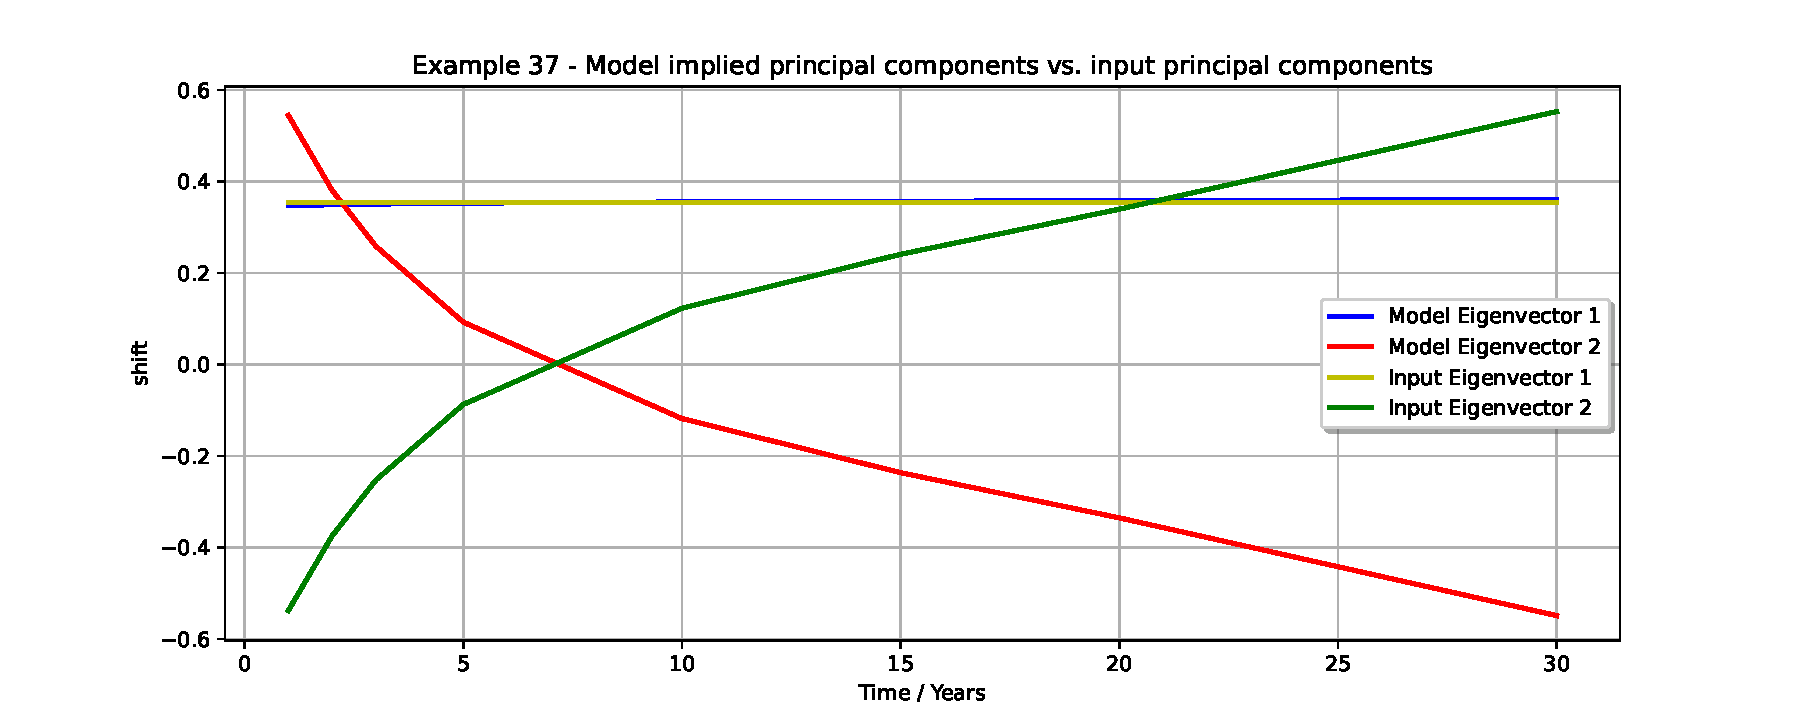
\includegraphics[scale=0.50]{examples/mpl_eigenvectors_ex37.pdf}
\end{center}
\caption{Input and model implied eigenvectors for a Hull-White 4-factor model calibrated to 2 principal components of
  rate curve movements (parallel + rotation). Notice that the model implied 2nd eigenvector is the negative of the input
  vector.}
\label{fig:ex37}
\end{figure}

%--------------------------------------------------------------------
\subsection{Cross Currency Swap Exposure using Multifactor Hull-White Models}% Example 38
\label{example:38}
%--------------------------------------------------------------------

The example in folder {\tt Examples/Example\_38} is similar to Example 8 (EPE, ENE for xccy swap), but uses a
multifactor HW model for EUR and USD to generate scenarios. The parametrization of the HW models is taken from Example
37.

Each of the two factors of each HW model is correlated with each of the two factors of the other currency's HW model and
with the FX factors. Remember that the factors represent principal components of interest rate movements and so the
correlations can be interpreted as correlations of these principal components with each other and the fx rate processes.

%--------------------------------------------------------------------
\subsection{Exposure Simulation using American Monte Carlo}% Example 39
\label{example:39}
%--------------------------------------------------------------------

The example in folder {\tt Examples/Example\_39} demonstrates how to use American Monte Carlo simulation (AMC) to generate exposures in ORE.
For a sketch of the methodology and comments on its implementation in ORE see \cite{methods}.

Calling 

\medskip
\centerline {\tt python run.py} 

\medskip
performs two ORE runs, a 'classical' exposure simulation and an American Monte Carlo simulation, both on a quarterly simulation grid and for the same portfolio consisting of four trades:

\begin{itemize}
\item Bermudan swaption
\item Single Currency Swap
\item Cross Currency Swap
\item FX Option
\end{itemize}

We use a 'flat' market here (yield curve and Swaption volatility surface). The number of simulation paths is 2k in the classic simulations. If not stated otherwise below, the number of training paths and simulation paths is 10k in the AMC simulations. 

In the following we compare the AMC exposure profiles to those produced by the 'classic' valuation engine for each trade and the netting set. 

Figure \ref{epe_swaption} shows the EPE and ENE for a Bermudan Swaption 10y into 10y in (base ccy) EUR with physical settlement. The classic run uses
the LGM grid engine for valuation. We observe close agreement between the two runs. To achieve the observed agreement, it is essential to set the LGM model's mean reversion speed to zero in both
\begin{itemize}
\item the Bermudan Swaption LGM pricing model (see Input/pricingengine.xml), and
\item the Cross Asset Model's IR model components (see Input/simulation.xml and Input/simulation\_amc.xml) 
\end{itemize}
and to use a high order 6 of the regression polynomials (see Input/pricingengine\_amc.xml).
 
\begin{figure}
  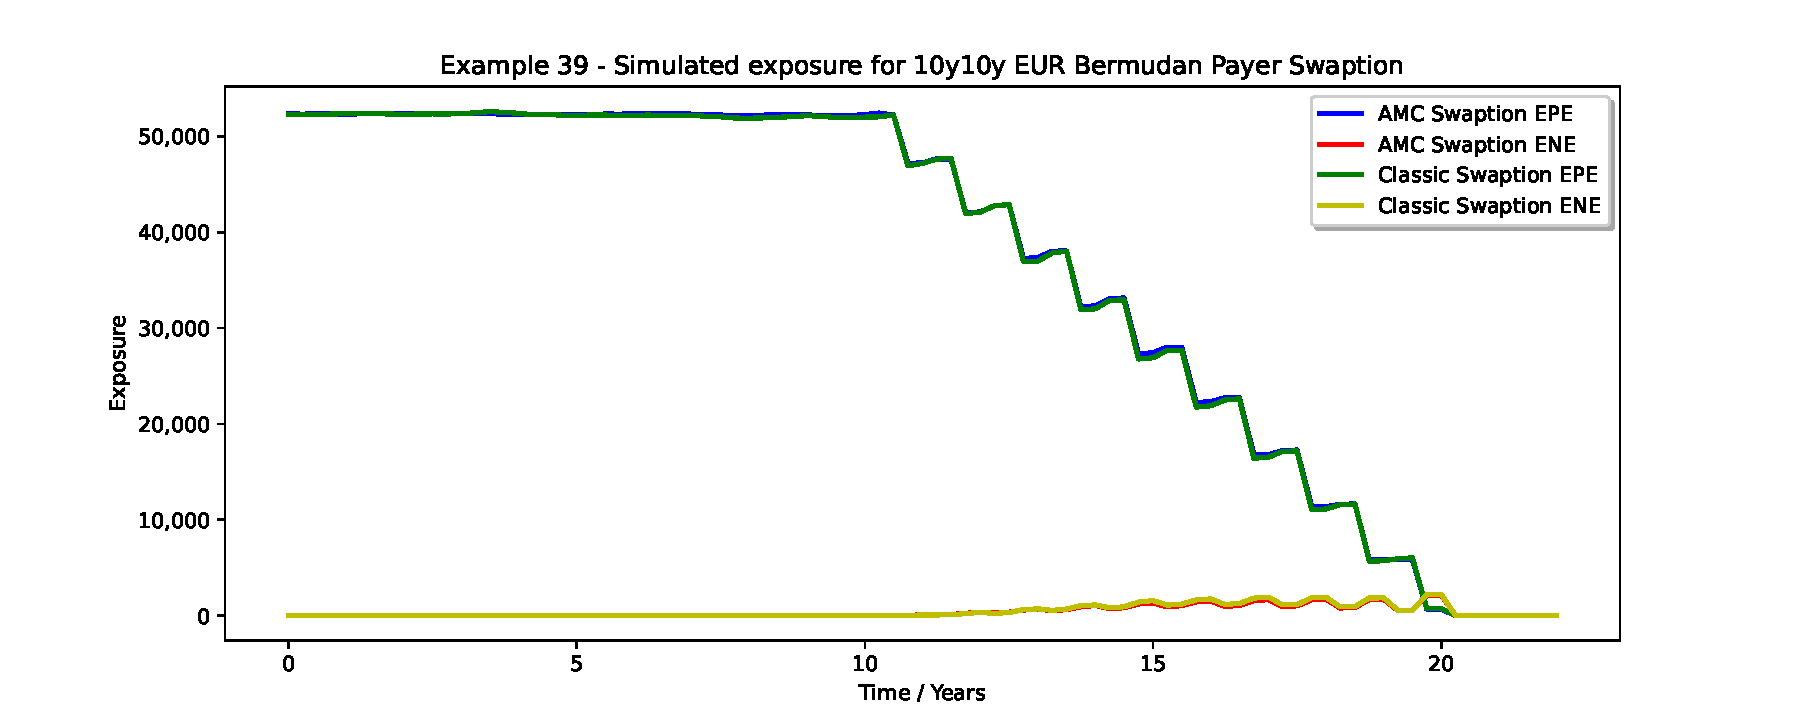
\includegraphics[width=0.8\textwidth]{examples/mpl_amc_bermudanswaption.pdf}
  \caption{EPE of a EUR Bermudan Swaption computed with the classic and AMC valuation engines, using 50k training paths for the AMC simulation.}
  \label{epe_swaption}
\end{figure}

Figure \ref{epe_swap} shows the EPE and ENE for a 20y vanilla Swap in USD. The currency of
the amc calculator is USD in this case, i.e. it is different from the base ccy of the simulation (EUR). The consistency
of the classic and amc runs in particular demonstrates the correct application of the currency conversion factor (see methodology guide).
To get a better accuracy for purposes of the plot in this document we increased the
number of training paths for this example to 50k and the order of the basis functions to 6.

\begin{figure}
  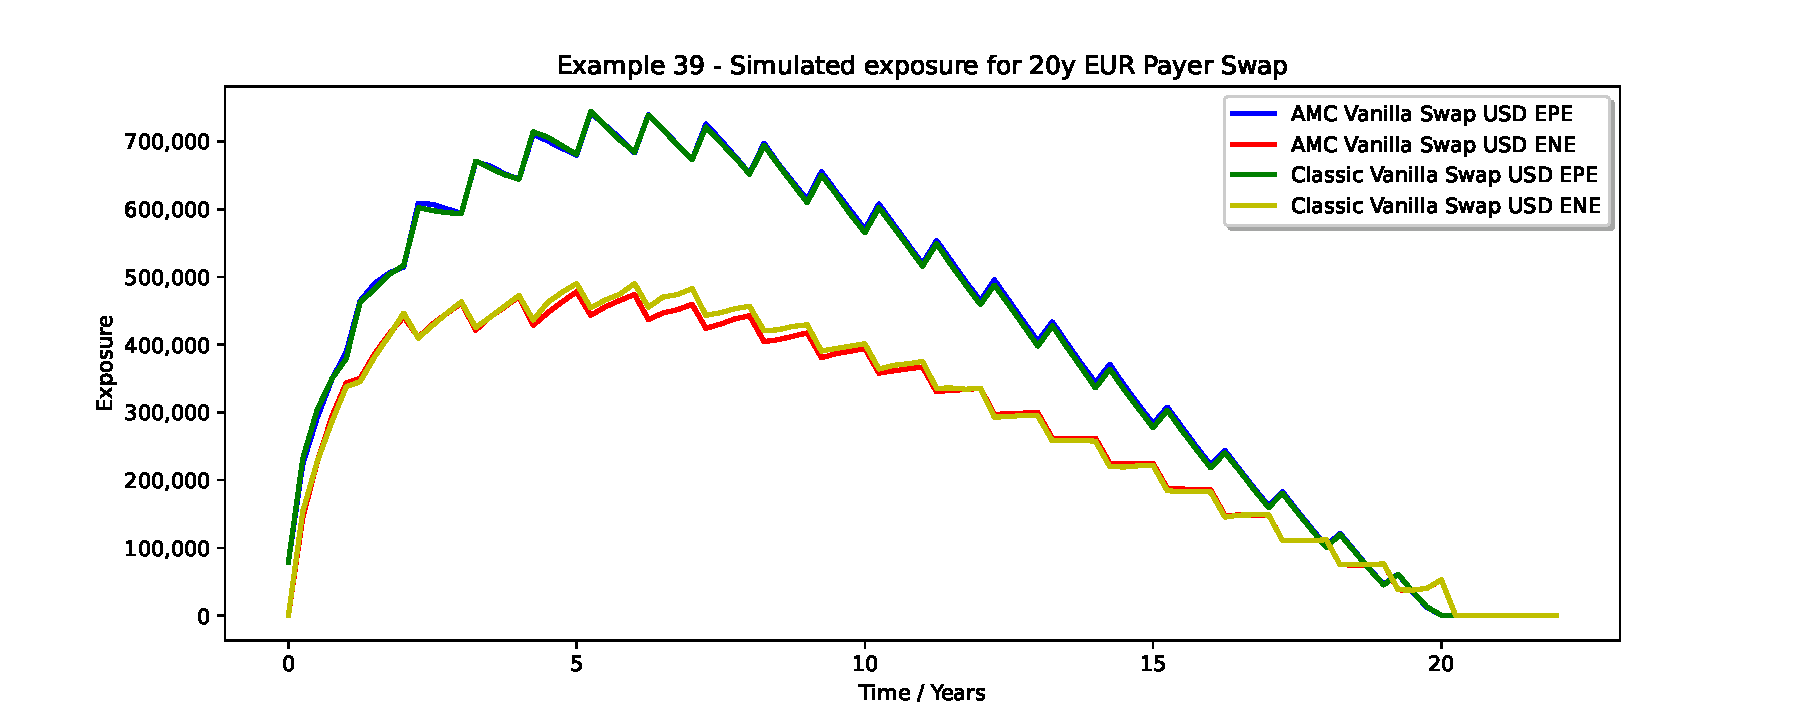
\includegraphics[width=0.8\textwidth]{examples/mpl_amc_vanillaswap_usd.pdf}
  \caption{EPE of a USD swap computed with the classic and AMC valuation engines}
  \label{epe_swap}
\end{figure}

Figure \ref{epe_ccyswap} shows the EPE and ENE for a 20y cross currency Swap EUR-USD. 

\begin{figure}
  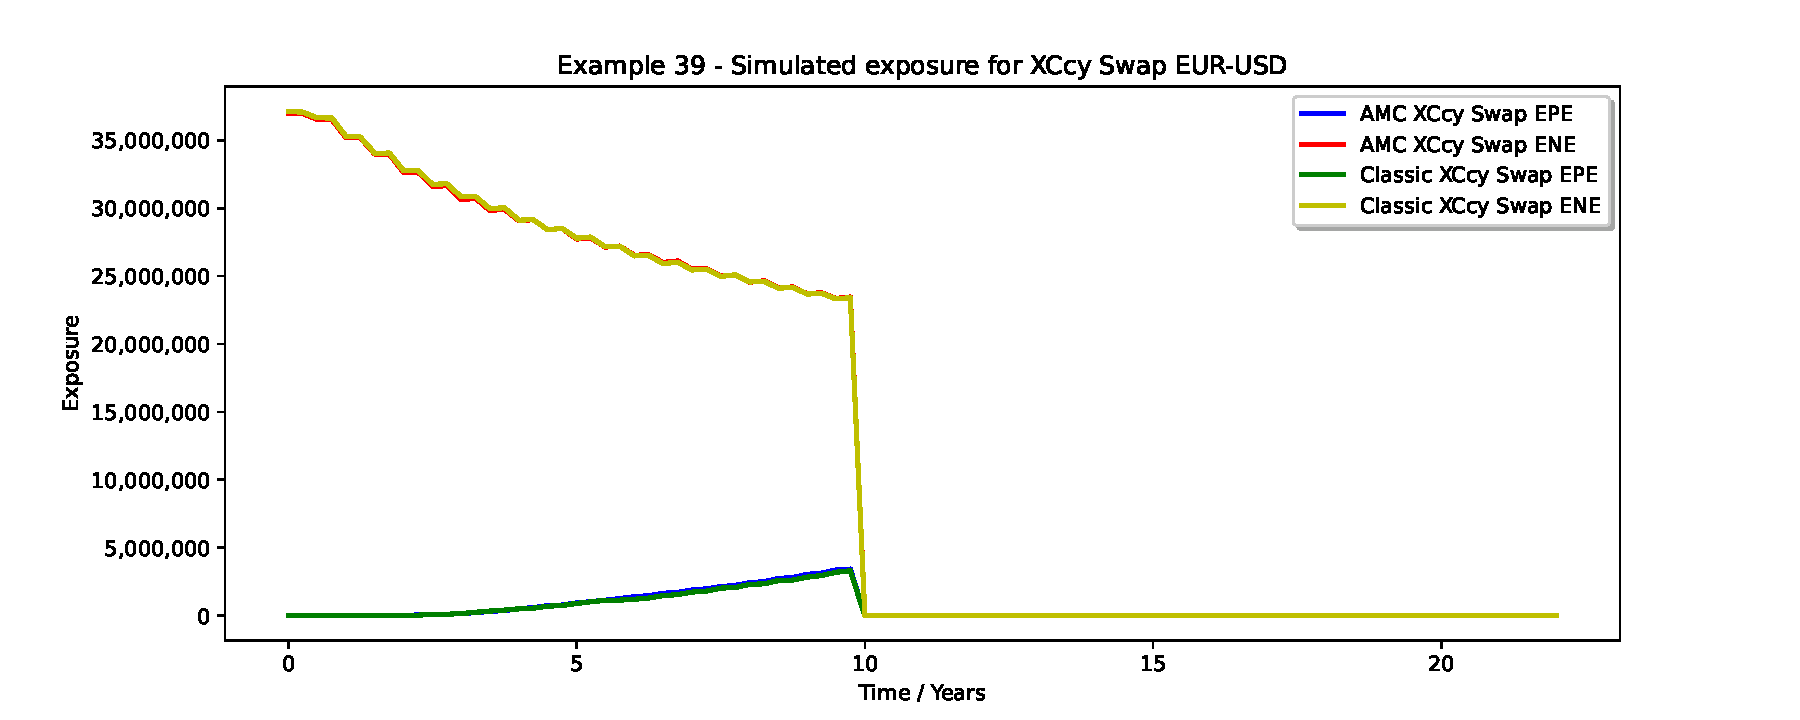
\includegraphics[width=0.8\textwidth]{examples/mpl_amc_xccyswap.pdf}
  \caption{EPE of a EUR-USD cross currency swap computed with the classic and AMC valuation engines}
  \label{epe_ccyswap}
\end{figure}

Figure \ref{epe_fxoption} shows the EPE and ENE for a vanilla FX Option EUR-USD with 10y1m expiry. 
For the classic run the FX volatility surface is not implied by the cross asset model but kept flat, which
yields a slight hump in the profile. The AMC profile is flat on the other hand which demonstrates the consistency of the
FX Option pricing with the risk factor evolution model.

\begin{figure}
  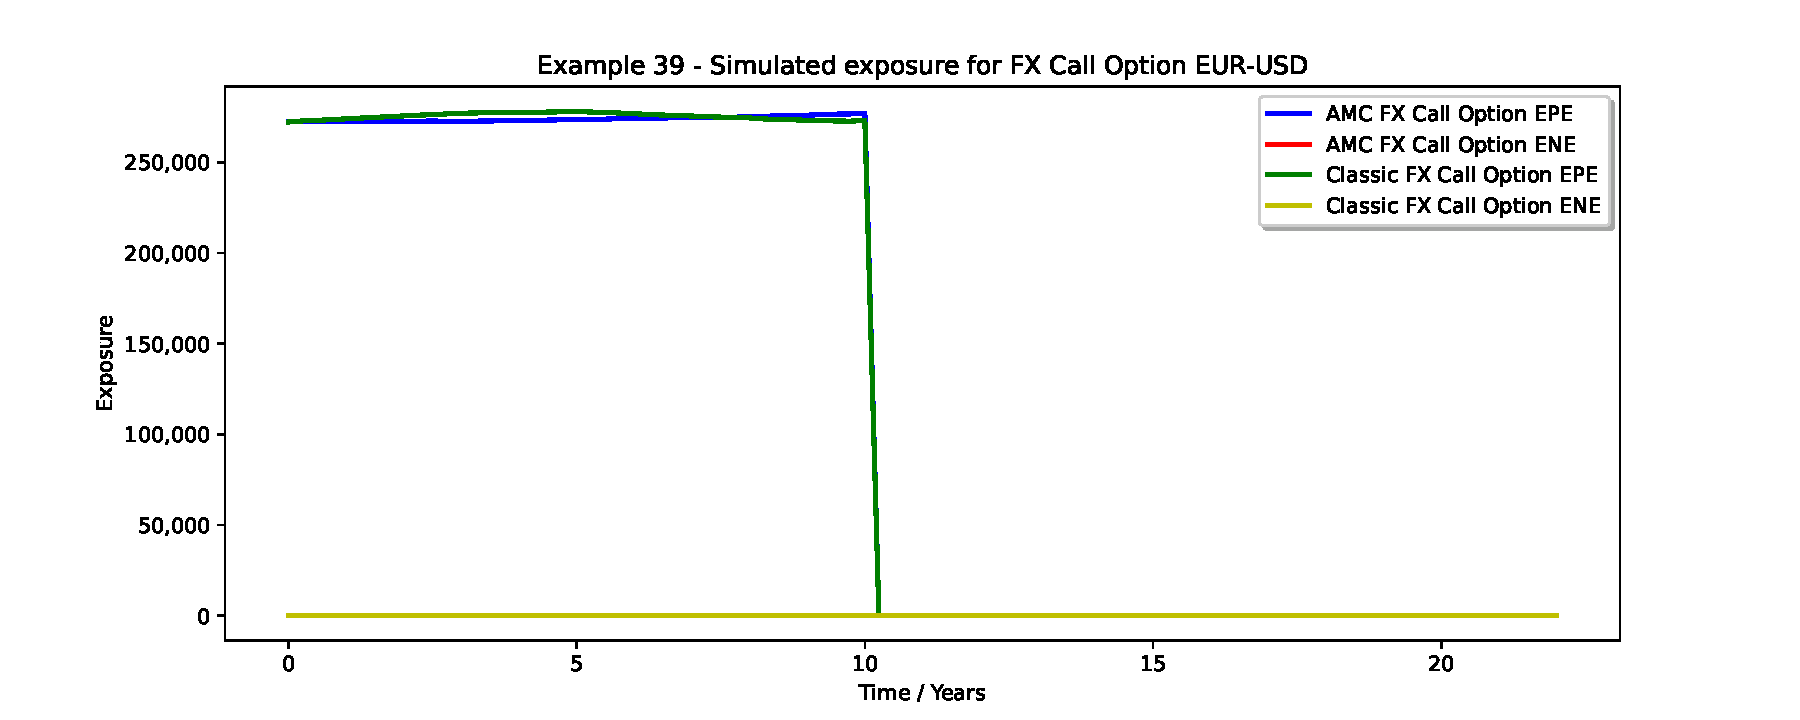
\includegraphics[width=0.8\textwidth]{examples/mpl_amc_fxoption.pdf}
  \caption{EPE of a EUR-USD FX option computed with the classic and AMC valuation engines}
  \label{epe_fxoption}
\end{figure}

\subsubsection*{Analytic Configuration}
\label{sec:amc_applicationconfig}

To use the AMC engine for an XVA simulation the following needs to be added to the {\tt simulation} analytic in {\tt ore.xml}:

\begin{minted}[fontsize=\scriptsize]{xml}
<Analytic type="simulation">
  ...
  <Parameter name="amc">Y</Parameter>
  <Parameter name="amcPricingEnginesFile">pricingengine_amc.xml</Parameter>
  <Parameter name="amcTradeTypes">Swaption</Parameter>
  ...
</Analytic>
\end{minted}

The trades which have a trade type matching one of the types in the \verb+amcTradeTypes+ list, will be built against the
pricing engine config provided and processed in the AMC engine. As a naming convention, pricing engines with engine type
AMC provide the required functionality to be processed by the AMC engine, for technical details cf. \cite{methods}.

All other trades are processed by the classic simulation engine in ORE. The resulting cubes from the classic and AMC
simulation are joined and passed to the post processor in the usual way.

Note that since sometimes the AMC pricing engines have a different base ccy than the risk factor evolution model (see
below), a horizon shift parameter in the simulation set up should be set for all currencies, so that the shift also
applies to these reduced models.

\subsubsection*{Pricing Engine Configuration}
\label{sec:amc_pricingengineconfig}

At this point we assume that the reader is generally familiar with the configuration section 
\ref{sec:configuration}, in particular pricing engine configuration in section in \cite{products}.

The pricing engine configuration is similar for all AMC enabled products, e.g. for Bermudan Swaptions:

\begin{minted}[fontsize=\scriptsize]{xml}
<Product type="BermudanSwaption">
  <Model>LGM</Model>
  <ModelParameters/>
  <Engine>AMC</Engine>
  <EngineParameters>
    <Parameter name="Training.Sequence">MersenneTwisterAntithetic</Parameter>
    <Parameter name="Training.Seed">42</Parameter>
    <Parameter name="Training.Samples">50000</Parameter>
    <Parameter name="Training.BasisFunction">Monomial</Parameter>
    <Parameter name="Training.BasisFunctionOrder">6</Parameter>
    <Parameter name="Pricing.Sequence">SobolBrownianBridge</Parameter>
    <Parameter name="Pricing.Seed">17</Parameter>
    <Parameter name="Pricing.Samples">0</Parameter>
    <Parameter name="BrownianBridgeOrdering">Steps</Parameter>
    <Parameter name="SobolDirectionIntegers">JoeKuoD7</Parameter>
    <Parameter name="MinObsDate">true</Parameter>
    <Parameter name="RegressionOnExerciseOnly">false</Parameter>
  </EngineParameters>
</Product>
\end{minted}

The \verb+Model+ differs by product type, table \ref{tbl:amcconfig} summarises the supported product types and model and
engine types. The engine parameters are the same for all products:

\begin{enumerate}
\item \verb+Training.Sequence+: The sequence type for the traning phase, can be \verb+MersenneTwister+,
  \verb+MersenneTwisterAntithetc+, \verb+Sobol+, \verb+Burley2020Sobol+, \verb+SobolBrownianBridge+,
  \verb+Burley2020SobolBrownianBridge+
\item \verb+Training.Seed+: The seed for the random number generation in the training phase
\item \verb+Training.Samples+: The number of samples to be used for the training phase
\item \verb+Pricing.Sequence+: The sequence type for the pricing phase, same values allowed as for training
\item \verb+Training.BasisFunction+: The type of basis function system to be used for the regression analysis, can be
  \verb+Monomial+, \verb+Laguerre+, \verb+Hermite+, \verb+Hyperbolic+, \verb+Legendre+, \verb+Chbyshev+,
  \verb+Chebyshev2nd+
\item \verb+BasisFunctionOrder+: The order of the basis function system to be used
\item \verb+Pricing.Seed+: The seed for the random number generation in the pricing
\item \verb+Pricing.Samples+: The number of samples to be used for the pricing phase. If this number is zero, no pricing
  run is performed, instead the (T0) NPV is estimated from the training phase (this result is used to fill the T0 slice
  of the NPV cube)
\item \verb+BrownianBridgeOrdering+: variate ordering for Brownian bridges, can be \verb+Steps+, \verb+Factors+,
  \verb+Diagonal+
\item \verb+SobolDirectionIntegers+: direction integers for Sobol generator, can be \verb+Unit+, \verb+Jaeckel+,
  \verb+SobolLevitan+, \verb+SobolLevitanLemieux+, \verb+JoeKuoD5+, \verb+JoeKuoD6+, \verb+JoeKuoD7+,
  \verb+Kuo+, \verb+Kuo2+, \verb+Kuo3+
\item \verb+MinObsDate+: if true the conditional expectation of each cashflow is taken from the minimum possible
  observation date (i.e. the latest exercise or simulation date before the cashflow's event date); recommended setting
  is \verb+true+
\item \verb+RegressionOnExerciseOnly+: if true, regression coefficients are computed only on exercise dates and
  extrapolated (flat) to earlier exercise dates; only for backwards compatibility to older versions of the AMC module,
  recommended setting is \verb+false+
\end{enumerate}

\begin{table}[hbt]
  \begin{tabular}{l|l|l}
    Product Type & Model & Engine \\ \hline
    Swap & CrossAssetModel & AMC \\
    CrossCurrencySwap & CrossAssetModel & AMC \\
    FxOption & CrossAssetModel & AMC \\
    BermudanSwaption & LGM & AMC \\
    MultiLegOption & CrossAssetModel & AMC \\
  \end{tabular}
  \caption{AMC enabled products with engine and model types}
  \label{tbl:amcconfig}
\end{table}

\subsubsection*{Additional Features}
\label{sec:amc_sideproducts}

As a side product the AMC module provides plain MC pricing engines for Bermudan Swaptions and a new trade type
\verb+MultiLegOption+ with a corresponding MC pricing engine.

\subsubsection*{MC pricing engine for Bermudan swaptions}\label{sec:mc_bermudan_engine}

The following listing shows a sample configuration for the MC Bermudan Swaption engine. The model parameters are
identical to the LGM Grid engine configuration. The engine parameters on the other hand are the same as for the AMC
engine, see \ref{sec:amc_pricingengineconfig}.

\begin{minted}[fontsize=\scriptsize]{xml}
<Product type="BermudanSwaption">
  <Model>LGM</Model>
  <ModelParameters>
    <Parameter name="Calibration">Bootstrap</Parameter>
    <Parameter name="CalibrationStrategy">CoterminalDealStrike</Parameter>
    <Parameter name="Reversion_EUR">0.0050</Parameter>
    <Parameter name="Reversion_USD">0.0030</Parameter>
    <Parameter name="ReversionType">HullWhite</Parameter>
    <Parameter name="VolatilityType">HullWhite</Parameter>
    <Parameter name="Volatility">0.01</Parameter>
    <Parameter name="ShiftHorizon">0.5</Parameter>
    <Parameter name="Tolerance">1.0</Parameter>
  </ModelParameters>
  <Engine>MC</Engine>
  <EngineParameters>
    <Parameter name="Training.Sequence">MersenneTwisterAntithetic</Parameter>
    <Parameter name="Training.Seed">42</Parameter>
    <Parameter name="Training.Samples">10000</Parameter>
    <Parameter name="Training.BasisFunction">Monomial</Parameter>
    <Parameter name="Training.BasisFunctionOrder">6</Parameter>
    <Parameter name="Pricing.Sequence">SobolBrownianBridge</Parameter>
    <Parameter name="Pricing.Seed">17</Parameter>
    <Parameter name="Pricing.Samples">25000</Parameter>
    <Parameter name="BrownianBridgeOrdering">Steps</Parameter>
    <Parameter name="SobolDirectionIntegers">JoeKuoD7</Parameter>
  </EngineParameters>
</Product>
\end{minted}

\subsubsection*{Multi Leg Options / MC pricing engine}

The following listing shows a sample MultiLegOption trade. It consists of

\begin{enumerate}
\item an option data block; this is optional, see below
\item a number of legs; in principle all leg types are supported, the number of legs is arbitrary and they can be in
  different currencies; if the payment currency of a leg is different from a floating index currency, this is
  interpreted as a quanto payoff
\end{enumerate}

If the option block is given, the trade represents a Bermudan swaption on the underlying legs. If the option block is
missing, the legs themselves represent the trade.

See \cite{methods} for limitations of the multileg option pricing engine.

\begin{minted}[fontsize=\scriptsize]{xml}
<Trade id="Sample_MultiLegOption">
  <TradeType>MultiLegOption</TradeType>
  <Envelope>...</Envelope>
  <MultiLegOptionData>
    <OptionData>
      <LongShort>Long</LongShort>
      <OptionType>Call</OptionType>
      <Style>Bermudan</Style>
      <Settlement>Physical</Settlement>
      <PayOffAtExpiry>false</PayOffAtExpiry>
      <ExerciseDates>
        <ExerciseDate>2026-02-25</ExerciseDate>
        <ExerciseDate>2027-02-25</ExerciseDate>
        <ExerciseDate>2028-02-25</ExerciseDate>
      </ExerciseDates>
    </OptionData>
    <LegData>
      <LegType>Floating</LegType>
      <Payer>false</Payer>
      <Currency>USD</Currency>
      <Notionals>
        <Notional>100000000</Notional>
      </Notionals>
      ...
    </LegData>
    <LegData>
      <LegType>Floating</LegType>
      <Payer>true</Payer>
      <Currency>EUR</Currency>
      <Notionals>
        <Notional>100000000</Notional>
      </Notionals>
      ...
    </LegData>
  </MultiLegOptionData>
</Trade>
\end{minted}

The pricing engine configuration is similar to that of the MC Bermudan swaption engine, cf.
\ref{sec:mc_bermudan_engine}, also see the following listing.

\begin{minted}[fontsize=\scriptsize]{xml}
  <Product type="MultiLegOption">
  <Model>CrossAssetModel</Model>
  <ModelParameters>
    <Parameter name="Tolerance">0.0001</Parameter>
    <!-- IR -->
    <Parameter name="IrCalibration">Bootstrap</Parameter>
    <Parameter name="IrCalibrationStrategy">CoterminalATM</Parameter>
    <Parameter name="ShiftHorizon">1.0</Parameter>
    <Parameter name="IrReversion_EUR">0.0050</Parameter>
    <Parameter name="IrReversion_GBP">0.0070</Parameter>
    <Parameter name="IrReversion_USD">0.0080</Parameter>
    <Parameter name="IrReversion">0.0030</Parameter>
    <Parameter name="IrReversionType">HullWhite</Parameter>
    <Parameter name="IrVolatilityType">HullWhite</Parameter>
    <Parameter name="IrVolatility">0.0050</Parameter>
    <!-- FX -->
    <Parameter name="FxCalibration">Bootstrap</Parameter>
    <Parameter name="FxVolatility_EURUSD">0.10</Parameter>
    <Parameter name="FxVolatility">0.08</Parameter>
    <Parameter name="ExtrapolateFxVolatility_EURUSD">false</Parameter>
    <Parameter name="ExtrapolateFxVolatility">true</Parameter>
    <!-- Correlations IR-IR, IR-FX, FX-FX -->
    <Parameter name="Corr_IR:EUR_IR:GBP">0.80</Parameter>
    <Parameter name="Corr_IR:EUR_FX:GBPEUR">-0.50</Parameter>
    <Parameter name="Corr_IR:GBP_FX:GBPEUR">-0.15</Parameter>
  </ModelParameters>
  <Engine>MC</Engine>
  <EngineParameters>
    <Parameter name="Training.Sequence">MersenneTwisterAntithetic</Parameter>
    <Parameter name="Training.Seed">42</Parameter>
    <Parameter name="Training.Samples">10000</Parameter>
    <Parameter name="Pricing.Sequence">SobolBrownianBridge</Parameter>
    <Parameter name="Pricing.Seed">17</Parameter>
    <Parameter name="Pricing.Samples">25000</Parameter>
    <Parameter name="Training.BasisFunction">Monomial</Parameter>
    <Parameter name="Training.BasisFunctionOrder">4</Parameter>
    <Parameter name="BrownianBridgeOrdering">Steps</Parameter>
    <Parameter name="SobolDirectionIntegers">JoeKuoD7</Parameter>
  </EngineParameters>
</Product>
\end{minted}

Model Parameters special to that product are

\begin{enumerate}
\item \verb+IrCalibrationStrategy+ can be \verb+None+, \verb+CoterminalATM+, \verb+UnderlyingATM+
\item \verb+FXCalibration+ can be \verb+None+ or \verb+Bootstrap+
\item \verb+ExtrapolateFxVolatility+ can be \verb+true+ or \verb+false+; if false, no calibration instruments are used
  that require extrapolation of the market fx volatilty surface in option expiry direction
\item \verb+Corr_Key1_Key2+: These entries describe the cross asset model correlations to be used; the syntax for
  \verb+Key1+ and \verb+Key2+ is the same as in the simulation configuration for the cross asset model
\end{enumerate}

%--------------------------------------------------------------------
\subsection{Par Sensitivity Analysis}% Example 40
\label{example:40}
%--------------------------------------------------------------------

The example in folder {\tt Examples/Example\_40}  demonstrates ORE's par sensitivity analysis (e.g. to Swap rates) 
that is implemented  by means of a Jacobi transformation of the "raw" sensitivities (e.g. to zero rates), see a sketch of the 
methodology in \cite{methods} and section \ref{sec:sensitivity} for configuration details.

To perform a par sensitivity analysis, the following required change in {\tt ore.xml} is required

\begin{minted}[fontsize=\scriptsize]{xml}
    <Analytic type="sensitivity">
      <Parameter name="active">Y</Parameter>
      <Parameter name="marketConfigFile">simulation.xml</Parameter>
      <Parameter name="sensitivityConfigFile">sensitivity.xml</Parameter>
      <Parameter name="pricingEnginesFile">../../Input/pricingengine.xml</Parameter>
      <Parameter name="scenarioOutputFile">sensi_scenarios.csv</Parameter>
      <Parameter name="sensitivityOutputFile">sensitivity.csv</Parameter>
      <Parameter name="outputSensitivityThreshold">0.000001</Parameter>
      <!-- Additional parametrisation for par sensitivity analysis -->
      <Parameter name="parSensitivity">Y</Parameter>
      <Parameter name="parSensitivityOutputFile">parsensitivity.csv</Parameter>
      <Parameter name="outputJacobi">Y</Parameter>
      <Parameter name="jacobiOutputFile">jacobi.csv</Parameter>
      <Parameter name="jacobiInverseOutputFile">jacobi_inverse.csv</Parameter>
    </Analytic>
\end{minted}

The portfolio used in this example includes products sensitive to 
\begin{itemize}
\item Discount and index curves
\item Credit curves
\item Inflation curves
\item CapFloor volatilities
\end{itemize}

The usual sensitivity analysis is performed by bumping the "raw" rates (zero rates, hazard rates, inflation zero rates, optionlet vols).
This is followed by the Jacobi transformation that turns "raw" sensitivities  into sensitivities in the par domain (Deposit/FRA/Swap rates, FX Forwards, CC Basis Swap spreads, 
CDS spreads, ZC and YOY Inflation Swap rates, flat Cap/Floor vols). The conversion is controlled by the additional {\tt ParConversion} data blocks 
in {\tt sensitivity.xml} where the assumed par instruments and corresponding conventions are coded, as shown below for three types of discount curves.

\begin{minted}[fontsize=\scriptsize]{xml}
  <DiscountCurves>
  
    <DiscountCurve ccy="EUR">
      <ShiftType>Absolute</ShiftType>
      <ShiftSize>0.0001</ShiftSize>
      <ShiftTenors>2W,1M,3M,6M,9M,1Y,2Y,3Y,4Y,5Y,7Y,10Y,15Y,20Y,25Y,30Y</ShiftTenors>
      <ParConversion>
        <!--DEP, FRA, IRS, OIS, FXF, XBS -->
	<Instruments>OIS,OIS,OIS,OIS,OIS,OIS,OIS,OIS,OIS,OIS,OIS,OIS,OIS,OIS,OIS,OIS</Instruments>
	<SingleCurve>true</SingleCurve>
	<Conventions>
	  <Convention id="OIS">EUR-OIS-CONVENTIONS</Convention>
	</Conventions>
      </ParConversion>
    </DiscountCurve>   
    
    <DiscountCurve ccy="USD">
      <ShiftType>Absolute</ShiftType>
      <ShiftSize>0.0001</ShiftSize>
      <ShiftTenors>2W,1M,3M,6M,9M,1Y,2Y,3Y,4Y,5Y,7Y,10Y,15Y,20Y,25Y,30Y</ShiftTenors>
      <ParConversion>
	<Instruments>FXF,FXF,FXF,FXF,FXF,XBS,XBS,XBS,XBS,XBS,XBS,XBS,XBS,XBS,XBS,XBS</Instruments>
	<SingleCurve>true</SingleCurve>
	<Conventions>
	  <Convention id="XBS">EUR-USD-XCCY-BASIS-CONVENTIONS</Convention>
	  <Convention id="FXF">EUR-USD-FX-CONVENTIONS</Convention>
	</Conventions>
      </ParConversion>

    <DiscountCurve ccy="GBP">
      <ShiftType>Absolute</ShiftType>
      <ShiftSize>0.0001</ShiftSize>
      <ShiftTenors>2W,1M,3M,6M,9M,1Y,2Y,3Y,4Y,5Y,7Y,10Y,15Y,20Y,25Y,30Y</ShiftTenors>
      <ParConversion>
	<Instruments>DEP,DEP,DEP,DEP,DEP,IRS,IRS,IRS,IRS,IRS,IRS,IRS,IRS,IRS,IRS,IRS</Instruments>
	<SingleCurve>true</SingleCurve>
	<Conventions>
	  <Convention id="DEP">GBP-DEPOSIT</Convention>
	  <Convention id="IRS">GBP-6M-SWAP-CONVENTIONS</Convention>
	</Conventions>
      </ParConversion>
    </DiscountCurve>
  
  </DiscountCurves>
\end{minted}

Finally note that par sensitivity analysis requires that the shift tenor grid in the sensitivity data above matches the corresponding grid in the simulation (market) configuration.
See also section \ref{sec:sensitivity}.

%--------------------------------------------------------------------
\subsection{Multi-threaded Exposure Simultion}% Example 41
\label{example:41}
%--------------------------------------------------------------------

The example in folder {\tt Examples/Example\_41} demonstrates the multithreaded valuation engine to generate the exposure for a
portfolio of 8 copies of the vanilla swap in {\tt Example\_1}.

%--------------------------------------------------------------------
\subsection{ORE Python Module}% Example 42
\label{example:42}
%--------------------------------------------------------------------

Since release 9 (March 2023) we provide easy access to ORE via a pre-compiled Python module. Some example scripts using this ORE module are provided in this example, so change to this directory first

\medskip
{\tt cd Example\_42} 

\medskip
The examples require Python 3. The ORE Python module is then installed with a one-liner, see step 3 below. However, to separate ORE from any other Python environments on your machine, we recommend creating a virtual environment first. In that case the steps are as follows. 

\begin{enumerate}
\item To create a virtual environment: {\tt python -m venv env1} 
\item To activate this environment on Windows: {\tt .{\bs}env1{\bs}Scripts{\bs}activate.bat}  \\
or on macOS/Linux: {\tt ./env1/bin/activate }  
\item Then install the latest release of ORE:\\
{\tt pip install open-source-risk-engine } 
\item Try examples:\\
	\begin{itemize} 
	\item {\tt python ore.py} \\
	This demonstrates the Python-wrapped version of the ORE application that is also used in the command line application {\tt ore.exe}. We use it here to re-run the Swap exposure of {\tt Example\_1}. 
	\item {\tt python ore2.py} \\
	This extends the previous example and shows how to access and post-process ORE in-memory results in the Python framework without reading files. 
	\item {\tt python commodityforward.py} \\
	The ORE Python module also allows lower-level access to the QuantLib and QuantExt libraries, demonstrated here for a CommodityForward instrument defined in QuantExt. 
	Note that the ORE Python module contains the entire QuantLib Python functionality.
	\end{itemize}
	More use cases of the ORE Python module including Jupyter notebooks can be found in the ORE SWIG repository, in particular in folder OREAnalytics-SWIG/Python/Examples. 
\item You can deactivate the environment with {\tt deactivate} \\
or even fully remove the environment again by removing the {\tt env1} folder.
\end{enumerate}

Finally, you can build the Python module and installable packages yourself following the instructions in sections \ref{sec:oreswig} based on your local ORE code. 

%--------------------------------------------------------------------
\subsection{Credit Portfolio Model}% Example 43
\label{example:43}
%--------------------------------------------------------------------

The purpose of the credit portfolio model in ORE is to generate an integrated portfolio gain/loss distribution at a given future horizon which is driven by 
\begin{itemize}
\item credit defaults and rating migrations in Bonds and CDS, and 
\item the PnL of a portfolio of derivatives over the specified time horizon.
\end{itemize}
The model integrates Credit and Market Risk by jointly evolving systemic credit risk drivers alongside the usual risk factors in ORE's Cross Asset Model.
See also the separate documentation in Docs/UserGuide/creditmodel.tex.

By running \\
\medskip
\centerline{{\tt python run.py}} 

\medskip
this example demonstrates the model's outcome for seven demo portfolios

\begin{center}
\begin{tabular}{|l|l|l|l|}
\hline
Case & Credit Mode & Exposure Mode & Evaluation \\
\hline
\hline
Single Bond & Migration & Value & Analytic \\
\hline
Bond and Swap & Migration & Value & Analytic \\
\hline
3 Bonds & Migration & Value & Analytic \\
\hline
10 Bonds & Migration & Value & Analytic \\
\hline
10 Bonds & Migration & Value & Terminal Simulation \\
\hline
Bonds and CDS & Migration & Notional & Analytic \\
\hline
100 Bonds & Default & Notional & Analytic \\
\hline
\end{tabular}
\end{center}
The last demo case in this table can be activated by uncommenting the corresponding section at the end of the {\tt run.py} script.
 
%--------------------------------------------------------------------
\subsection{Initial Margin: ISDA SIMM and IM Schedule}% Example 44
\label{example:44}
%--------------------------------------------------------------------

{\tt Example\_44} demonstrates the calculation of initial margin using ISDA's Standard Initial Margin Model (SIMM) based on a provided 
sensitivity file in ISDA's Common Risk Interchange Format (CRIF). In addition, we show how to use the standard "IM Schdule" method to compute 
initial margin.

ORE covers all SIMM versions since inception to date, i.e.\ 1.0, 1.1, 1.2, 1.3, 1.3.38, 2.0, 2.1, 2.2, 2.3, 2.4 (=2.3.8), 2.5, 2.5A, 2.6 (=2.5.6).
All versions have been tested against the respective ISDA SIMM model unit test suites and pass these tests.
Any new SIMM versions will be added with each ORE release.

For SIMM versions >= 2.2 we support SIMM calculation for both MPoR horizons, 1d and 10d.
 
Note that you need to purchase a SIMM model license from ISDA if you want to use the model in production, and the unit test
suites mentioned above are provided to licensed vendors only. Therefore we unfortunately cannot share our ORE SIMM model 
test suite here either. 

By running \\
\medskip
\centerline{{\tt python run.py}} 

\medskip
ORE will pick up the small example CRIF file in {\tt Input/crif.csv} (i.e.\ par sensitivities rebucketed and reformatted to match the ISDA CRIF template) and generate the resulting SIMM report in a {\tt simm.csv} file.
This report shows ISDA SIMM results with the usual breakdown by product class, risk class, margin type, bucket and SIMM ``side'' (IM to call or post).
The SIMM calculation in this example is done for SIMM version 2.4 and 2.6, with MPoR 1d and 10d:

\begin{itemize}
  \item SIMM 2.4, 1-day MPoR
  \item SIMM 2.4, 10-day MPoR
  \item SIMM 2.6, 1-day MPoR
  \item SIMM 2.6, 10-day MPoR
\end{itemize}

\medskip
There are four SIMM-related input files -- {\tt ore\_SIMM2.4\_1D.xml}, {\tt ore\_SIMM2.4\_10D.xml}, {\tt ore\_SIMM2.6\_1D.xml}, {\tt ore\_SIMM2.6\_10D.xml} -- with corresponding folders in the {\tt Output/} directory.
The relevant inputs in the files are:

\begin{itemize}
\item SIMM version
\item name of the CRIF file to be loaded
\item calculation currency - this determines which Risk\_FX entries of the CRIF will be ignored in the SIMM calculation
\item result currency (optional) - currency of the resulting SIMM amounts in the report, by default equal to the calculation currency
\item MPoR horizon, in terms of days
\end{itemize}

The market data input and todays's market configuration required here is minimal - limited to FX rates for conversions from base/calculation currency into USD and into the result currency.

\bigskip
If the ORE Python module is installed, as shown in Example 42, then you can also run the SIMM example using

\medskip
\centerline{\tt python ore.py} 

\subsubsection*{IM Schedule}

As an additonal case in this example we demonstrate how to use the IM Schedule method to compute initial margin.
The related input file is {\tt Input/ore\_schedule.xml}. It is also run when calling {\tt python run.py}, and results are written to folder 
{\tt Output/IM\_SCHEDULE}.
The basic input is provided in CRIF file format where ORE expects two lines per trade, one with RiskClass = PV and one with RiskClass = Notional, 
so that the  amounts in these CRIF lines are interpeted as NPV respectively notional. 
Further required columns are product class and end date, as shown in the example {\tt Input/crif\_schedule.csv}. Note that the product class has to be in
\begin{itemize}
  \item Rates
  \item FX
  \item Equity
  \item Credit
  \item Commodity
\end{itemize}
in contrast to SIMM where we use the combined RatesFX.

To run the IM Schedule analytic, the following minimal addition to {\tt Input/ore\_schedule.xml} is required.
\begin{minted}[fontsize=\scriptsize]{xml}
  <Analytics>
    <Analytic type="imschedule">
      <Parameter name="active">Y</Parameter>
      <Parameter name="crif">crif_schedule.csv</Parameter>
      <Parameter name="calculationCurrency">USD</Parameter>
    </Analytic>
  </Analytics>
\end{minted}

%--------------------------------------------------------
\subsection{Collateralized Bond Obligation}% Example 45
%--------------------------------------------------------

This example in folder {\tt Examples/Example\_45} demonstrates a Cashflow CDO or Collateralized Bond Obligation (CBO) via ORE. Calling

\medskip
\centerline{\tt python run.py}

\medskip
will launch a single ORE run to process a CBO example, referencing underyling bond portfolio of 20 trades. 
The CBO is represented by a CBO reference datum specified in the reference data file. 
NPV results are calculated for the investment in the junior tranche. 

%--------------------------------------------------------
\subsection{Generic Total Return Swap}% Example 46
%--------------------------------------------------------

This example in folder {\tt Examples/Example\_46} demonstrates ORE's generic Total Return Swap referencing a CBO. 
Calling

\medskip
\centerline{\tt python run.py}

\medskip
will launch a single ORE run to process a TRS example and to generate NPV and cash flows in the usual result files.
As opposed to example 45, the CBO and its bondbasket are represented explicitly in the CBO node.

%--------------------------------------------------------
\subsection{Composite Trade}% Example 47
%--------------------------------------------------------

This example in folder {\tt Examples/Example\_47} demonstrates the input of ORE's Composite Trade that can consist on any number 
and type of products covered by ORE. In this case the composite consists of two Equity Swaps.
Calling

\medskip
\centerline{\tt python run.py}

\medskip
runs ORE and generates an NPV report.

%--------------------------------------------------------
\subsection{Convertible Bond and ASCOT}% Example 48
%--------------------------------------------------------

This example in folder {\tt Examples/Example\_48} demonstrates the input of 
\begin{itemize}
\item a ConvertibleBond  trade
\item a related Asset Swapped Convertible Option Transaction (ASCOT)
\item a vanilla Swap that represents the package of Convertible Bond position and ASCOT
\end{itemize}

Calling
\medskip
\centerline{\tt python run.py}

\medskip
runs ORE and generates an NPV report.

%--------------------------------------------------------
\subsection{Bond Yield Shifted}% Example 49
\label{example:49}
%--------------------------------------------------------

The example in folder {\tt Examples/Example\_49} shows how to use a yield curve
built from a BondYieldShifted segment, as described in section \ref{sec:bond_yield_shifted}.

In particular, it builds the curve {\tt USD.BMK.GVN.CURVE\_SHIFTED} shifted by three liquid Bonds:

\begin{itemize}
\item Fixed rate USD Bond maturing in August 2023 with id {\tt EJ7706660}.
\item Fixed rate USD Bond maturing in September 2049 with id {\tt ZR5330686}.
\item Floating Rate Bond maturing in May 2025 with id {\tt AS064441}.
\end{itemize}

The resulting curve is exhibited in the {\tt curves.csv} output file.
Moreover, the results can be crosschecked against the NPVs, i.e. prices, of the ZeroBonds comprised in the portfolio.
\begin{itemize}
\item {\tt ZeroBond\_long}, maturing 2052-03-01 shows a price of 0.2080 akin to the 0.2080 in the curves output at the same date.
\item {\tt ZeroBond\_short}, maturing 2032-06-01 shows a price of 0.5808 aktin to the 0.808 in the curves output at the same date.
\end{itemize}

The example can be run calling {\tt python run.py}.


%--------------------------------------------------------------------
\subsection{Zero to Par sensitivity Conversion Analysis}% Example 50
\label{example:50}
%--------------------------------------------------------------------

The example in folder {\tt Examples/Example\_50} demonstrates ORE's capability to convert external computed zero sensitivities (e.g Zero rates) to par sensitivities (e.g. to Swap rates) 
that is implemented  by means of a Jacobi transformation of the "raw" sensitivities (e.g. to zero rates), see a sketch of the 
methodology in \cite{methods} and section \ref{sec:sensitivity} for configuration details.

To perform a par sensitivity analysis, the following required change in {\tt ore.xml} is required

\begin{minted}[fontsize=\scriptsize]{xml}
    <Analytic type="zeroToParSensiConversion">
      <Parameter name="active">Y</Parameter>
      <Parameter name="marketConfigFile">simulation.xml</Parameter>
      <Parameter name="sensitivityConfigFile">sensitivity.xml</Parameter>
      <Parameter name="pricingEnginesFile">../../Input/pricingengine.xml</Parameter>
	  <!-- Input file with the raw sensitivities -->
      <Parameter name="sensitivityInputFile">sensitivity.csv</Parameter>
      <Parameter name="idColumn">TradeId</Parameter>
      <Parameter name="riskFactorColumn">Factor_1</Parameter>
      <Parameter name="deltaColumn">Delta</Parameter>
	  <Parameter name="currencyColumn">Currency</Parameter>
	  <Parameter name="baseNpvColumn">Base NPV</Parameter>
 	  <Parameter name="shiftSizeColumn">ShiftSize_1</Parameter>
      <Parameter name="outputThreshold">0.000001</Parameter>
      <Parameter name="outputFile">parconversion_sensitivity.csv</Parameter>
      <Parameter name="outputJacobi">Y</Parameter>
      <Parameter name="jacobiOutputFile">jacobi.csv</Parameter>
      <Parameter name="jacobiInverseOutputFile">jacobi_inverse.csv</Parameter>
    </Analytic>
\end{minted}

The portfolio used in this example includes zero sensitivities of 
\begin{itemize}
\item Discount and index curves
\item Credit curves
\item Inflation curves
\item CapFloor volatilities
\end{itemize}

ORE reads the raw sensitivities from the csv input file *sensitivityInputFile*. The input file needs to have six  columns, the column names can be user configured. Here is a description of each of the columns:

\begin{enumerate}
\item idColumn : Column with a unique identifier for the trade / nettingset / portfolio.
\item riskFactorColumn: Column with the identifier of the zero/raw sensitivity. The risk factor name needs to follow the ORE naming convention, e.g. DiscountCurve/EUR/5/1Y (the 6th bucket in EUR discount curve as specified in the sensitivity.xml)\
\item deltaColumn: The raw sensitivity of the trade/nettingset / portfolio with respect to the risk factor
\item currencyColumn: The currency in which the raw sensitivity is expressed, need to be the same as the BaseCurrency in the simulation settings.
\item shiftSizeColumn: The shift size applied to compute the raw sensitivity, need to be consistent to the sensitivity configuration.
\item baseNpvColumn: The base npv of the trade / nettingset / portfolio in currency.
\end{enumerate}

This is followed by the Jacobi transformation that turns "raw" sensitivities  into sensitivities in the par domain (Deposit/FRA/Swap rates, FX Forwards, CC Basis Swap spreads, 
CDS spreads, ZC and YOY Inflation Swap rates, flat Cap/Floor vols). The conversion is controlled by the additional {\tt ParConversion} data blocks 
in {\tt sensitivity.xml} where the assumed par instruments and corresponding conventions are coded, as shown below for three types of discount curves.

\begin{minted}[fontsize=\scriptsize]{xml}
  <DiscountCurves>
  
    <DiscountCurve ccy="EUR">
      <ShiftType>Absolute</ShiftType>
      <ShiftSize>0.0001</ShiftSize>
      <ShiftTenors>2W,1M,3M,6M,9M,1Y,2Y,3Y,4Y,5Y,7Y,10Y,15Y,20Y,25Y,30Y</ShiftTenors>
      <ParConversion>
        <!--DEP, FRA, IRS, OIS, FXF, XBS -->
	<Instruments>OIS,OIS,OIS,OIS,OIS,OIS,OIS,OIS,OIS,OIS,OIS,OIS,OIS,OIS,OIS,OIS</Instruments>
	<SingleCurve>true</SingleCurve>
	<Conventions>
	  <Convention id="OIS">EUR-OIS-CONVENTIONS</Convention>
	</Conventions>
      </ParConversion>
    </DiscountCurve>   
    
    <DiscountCurve ccy="USD">
      <ShiftType>Absolute</ShiftType>
      <ShiftSize>0.0001</ShiftSize>
      <ShiftTenors>2W,1M,3M,6M,9M,1Y,2Y,3Y,4Y,5Y,7Y,10Y,15Y,20Y,25Y,30Y</ShiftTenors>
      <ParConversion>
	<Instruments>FXF,FXF,FXF,FXF,FXF,XBS,XBS,XBS,XBS,XBS,XBS,XBS,XBS,XBS,XBS,XBS</Instruments>
	<SingleCurve>true</SingleCurve>
	<Conventions>
	  <Convention id="XBS">EUR-USD-XCCY-BASIS-CONVENTIONS</Convention>
	  <Convention id="FXF">EUR-USD-FX-CONVENTIONS</Convention>
	</Conventions>
      </ParConversion>

    <DiscountCurve ccy="GBP">
      <ShiftType>Absolute</ShiftType>
      <ShiftSize>0.0001</ShiftSize>
      <ShiftTenors>2W,1M,3M,6M,9M,1Y,2Y,3Y,4Y,5Y,7Y,10Y,15Y,20Y,25Y,30Y</ShiftTenors>
      <ParConversion>
	<Instruments>DEP,DEP,DEP,DEP,DEP,IRS,IRS,IRS,IRS,IRS,IRS,IRS,IRS,IRS,IRS,IRS</Instruments>
	<SingleCurve>true</SingleCurve>
	<Conventions>
	  <Convention id="DEP">GBP-DEPOSIT</Convention>
	  <Convention id="IRS">GBP-6M-SWAP-CONVENTIONS</Convention>
	</Conventions>
      </ParConversion>
    </DiscountCurve>
  
  </DiscountCurves>
\end{minted}

Finally note that par sensitivity analysis requires that the shift tenor grid in the sensitivity data above matches the corresponding grid in the simulation (market) configuration. 
See also section \ref{sec:sensitivity}.


%--------------------------------------------------------------------
\subsection{Custom Trade Fixings}% Example 51
\label{example:51}
%--------------------------------------------------------------------

The example in folder {\tt Examples/Example\_51} demonstrates ORE's capability to use custom trade specific fixings. For OIS and Ibor floating legs one can specify historical fixing on a trade level, see FloatingLeg data in \cite{products}. Those trade level fixings will be only use for the specific trade, all other trades will use the global fixings.

%--------------------------------------------------------------------
\subsection{Scripted Trade}% Example 52
\label{example:52}
%--------------------------------------------------------------------

The scripted trade was added to ORE to gain more flexibility in representing exotic products, with hyprid payoffs across
asset classes, path-dependence, multiple kinds of early termination options. The scripted trade module uses Monte Carlo and
Finite Difference pricing approaches, it is an evolving interface to implement parallel processing with GPUs and a central
interface to implement AD methods in ORE. See the separate documentation in folder Docs/ScriptedTrade for an introduction to trade
representation, scripting language, model and pricing engine configuration. 

\medskip
The example in this folder {\tt Examples/Example\_52} is a basic demonstration of ORE's scripted trade functionality.
In this example we provide a self-contained case that can be run as usual calling

\medskip
\centerline{\tt python run.py}

\medskip

This generates an NPV and cash flow report for the following portfolio
\begin{itemize}
\item Trade 1: Vanilla European Equity Option, represented as standard ORE XML with analytical pricing
\item Trade 2: Same Option as above, represented as ``generic'' scripted trade with scripted payoff embedded into the trade XML,
  pricing via Monte Carlo
\item Trade 3: Same Option as above, same representation, pricing via Finite Differences triggered by a {\tt ProductTag} assigned
  to the script and used in {\tt pricingengine.xml} 
\item Trade 4: Same Option as above, the scripted trade now refers to an ``external'' script in {\tt scriptlibrary.xml},
  MC pricing
\item Trade 4b: Same as trade 4, but ``compact'' scripted trade representation (uncomment trade 4b in {\tt portfolio.xml})
\item Trade 5: Barrier Option with single continuously observed Up \& Out barrier, represented as standard ORE XML with
  analytical pricing
\item Trade 6: Same Barrier Option as above, approximated as generic scripted trade with daily barrier observation
\item Trade 6b: Same Barrier Option as above, approximated as ``compact'' scripted trade with daily barrier observation
  (uncomment trade 6b in {\tt portfolio.xml})
\item Trade 7: Same Barrier Option as above, represented as generic scripted trade with continuously observed barrier,
  i.e. adjusting for the probability of knock-out between daily observations
\item Trade 7b: Same Barrier Option as of above, represented as ``compact'' scripted trade
  (uncomment trade 7b in {\tt portfolio.xml})
\item Trade 8: Equity Accumulator, represented as generic scripted trade with external payoff script
\item Trade 8b: Same Equity Accumulator as above, represented as compact scripted trade with external payoff script
  (uncomment trade 8b in {\tt portfolio.xml})
\end{itemize}

Note:
\begin{itemize}
\item In all cases we use the Black-Scholes model to drive the Equity process.
\item The Barrier Option pricing using the scripted trade deviates noticeably from the analytical pricing when we use daily
  observations (trade 6 and 6b), but matches quite closely when we adjust for the probability of knock-out between observation
  dates (trade 7 and 7b)
\item We are not aware of analytical pricing for the Accumulator product in trade 8 to benchmark against; trade 8 is priced with MC,
  FD pricing of the Accumulator is possible as well but requires a separate payoff script, only in the vanilla European option case
  we can utilize the same script for both MC and FD pricing
\end{itemize}

Though this initial Example\_52 shows only single-asset Equity cases, the scripted trade in its current version is
  significantly more versatile, more examples and scripts to follow.

%--------------------------------------------------------------------
\subsection{Curve Building around Central Bank Meeting Dates}% Example 53
\label{example:53}
%--------------------------------------------------------------------

This example demonstrates the build of a GBP OIS curve using MPC Swaps at the short end.

%--------------------------------------------------------------------
\subsection{Scripted Trade Exposure with AMC: Bermudan Swaption and LPI Swap}% Example 54
\label{example:54}
%--------------------------------------------------------------------

This example demonstrates exposure simulation using AMC for selected scripted trade types
\begin{itemize}
\item Bermudan Swaption
\item LPI Swap
\end{itemize}
Both payoffs are defined in {\tt scriptlibrary.xml} which is referenced in {\tt portfolio.xml}. \\

To enable the AMC processing requires the following highlighted settings in {\tt ore.xml}.

\begin{minted}[fontsize=\scriptsize]{xml}
    <Analytic type="simulation">
      <Parameter name="active">Y</Parameter>
      <!-- Set to Y to trigger AMC processing -->
      <Parameter name="amc">Y</Parameter>
      <Parameter name="simulationConfigFile">simulation.xml</Parameter>
      <Parameter name="pricingEnginesFile">pricingengine.xml</Parameter>
      <!-- Specify a separate pricing engine file for AMC engines -->
      <Parameter name="amcPricingEnginesFile">pricingengine\_amc.xml</Parameter>
      <!-- Specify trade types to be covered by the AMC processing -->
      <Parameter name="amcTradeTypes">ScriptedTrade</Parameter>
      <Parameter name="baseCurrency">EUR</Parameter>
      <Parameter name="cubeFile">cube.csv.gz</Parameter>
      <Parameter name="aggregationScenarioDataFileName">scenariodata.csv.gz</Parameter>
      <Parameter name="aggregationScenarioDataDump">scenariodata.csv</Parameter>
    </Analytic>
\end{minted}

Note that ORE can handle a mix of trades covered by AMC simulation and covered by ``classic'' simulation.
The respective NPV cubes are combined before generating results such as exposures or XVAs.

%--------------------------------------------------------------------
\subsection{Scripted Trade Exposure with AMC: Target Redemption Forward}% Example 55
\label{example:55}
%--------------------------------------------------------------------

This example in folder {\tt Examples/Example\_55} demonstrates exposure simulation and XVA for another scripted product, an
FX Target Redemption Forward (TaRF). In contrast to the cases presented above, you won't see
the payoff script library in the Input folder, nor is the script embedded into the trade XML file.
The trade type in this case is {\tt FxTARF} which has its own implementation in OREData/ored/portfolio/tarf.xpp
and a separate trade schema. However, the scipted trade framework is used under the hood, and the payoff
script is embedded into the C++ code in OREData/ored/portfolio/tarf.cpp.

%--------------------------------------------------------------------
\subsection{CVA Sensitivities using AAD}% Example 56
\label{example:56}
%--------------------------------------------------------------------

This example in folder {\tt Examples/Example\_56} demonstrates a prototype CVA sensitivity
calculation applying Adjoint Algorithmic Differentiation (AAD)
to a Swap instrument represented as scripted trade. 

%--------------------------------------------------------------------
\subsection{Base Scenario Analytic}% Example 57
\label{example:57}
%--------------------------------------------------------------------

{\tt Example\_57} demonstrates the {\tt Scenario} analytic which has been added to export the simulation market's base scenario
as a file.

%--------------------------------------------------------------------
\subsection{Historical Simlation VaR Analytic}% Example 58
\label{example:58}
%--------------------------------------------------------------------

This example in folder {\tt Examples/Example\_58} demonstrates a historical simulation VaR calculation
given a portfolio and externally provided ``market scenarios'' covering
one or several historical observation period(s).
The analytic is specified as usual in {\tt ore.xml} with the following parameters:
\begin{itemize}
\item outputFile: csv file name of the resulting VaR report 
%\item breakdown: boolean, if true the VaR report will contain a breakdown by risk class and risk type, otherwise the report shows the portfolio-lvel VaR only.
\item quantiles: comma searated list of quantiles to be reported
\item portfolioFilter (optional): Only trades with {\tt portfolioId} equal to the provided filter name are processed, see {\tt portfolio.xml}; the entire portfolio is processed, if omitted
\item historicalPeriod: comma-separated date list, an even number of ordered dates is required (d1, d2, d3, d4, ...), where each pair (d1-d2, d3-d4, ...) defines the start and end of historical observation periods used
\item mporDays: Number of calendar days between historical scenarios taken from the observation periods in order to compute P\&L effects (typically 1 or 10) 
\item mporCalendar: Calendar applied in the scenario date calculation
\item mporOverlappingPeriods: Boolean, if true we use overlapping periods of length mporDays (t to t + 10 calendate days, t+1 to t+11, t+2 to t+12, ...), otherwise consecutive periods (t to t+10, t+10 to t+20, ...)
\item simulationConfigFile: defines the structure of the simulation market applied in the P\&L calculation, e.g. discount and index curves, yield curve tenor points used, FX pairs etc.
\item historicalScenarioFile: csv file containing the market scenarios for each date in the observation periods defined below; the granularity of the scenarios (e.g. discount and index curves, number of yield curve tenors) needs to match the simulation market definition above; each yield curve tenor scenario is represented as a discount factor 
\end{itemize}

The example is run as usual by calling {\tt python run.py}

%--------------------------------------------------------------------
\subsection{SABR Model for Swaptions and Caps/Floors}% Example 59
\label{example:59}
%--------------------------------------------------------------------

This example in folder {\tt Examples/Example\_59} demonstrates the pricing of a Swaption and a Cap on
volatility surfaces that are interpolated in smile direction using a SABR
model flavour. As usual the example is run by calling {\tt python run.py}

The essential configuration is in {\tt curveconfig.xml} where the
Interpolation (Swaption) resp. StrikeInterpolation (Caps/Floors) allows
the following new SABR types
\begin{itemize}
\item Hagan2002Lognormal
\item Hagan2002Normal
\item Hagan2002NormalZeroBeta
\item Antonov2015FreeBoundaryNormal
\item KienitzLawsonSwaynePde
\item FlochKennedy
\end{itemize}
SABR parameters can be calibrated or have fixed externally provided values
per option tenor and Swap tenor (Swaptions) resp. optionlet (Caps/Floors).

%--------------------------------------------------------------------
\subsection{Overlapping Close-Out Grids}% Example 60
\label{example:60}
%--------------------------------------------------------------------

The example in folder {\tt Examples/Example\_60} demonstrates ORE's capability to handle xVA simulations using American Monte-Carlo with overlapping close-out grids.

%--------------------------------------------------------------------
\subsection{Fast Sensitivities using AAD and GPUs}% Example 61
\label{example:61}
%--------------------------------------------------------------------

This example in folder {\tt Examples/Example\_61} demonstrates alternative ways of speeding up sensitivity
calculations - using AAD or an external compute device.
The test portfolio consists of 
\begin{itemize}
\item Vanilla Equity Option
\item Equity Barrier Option
\item Equity Accumulator
\item Asian Basket Option
\item FX TaRFs
\end{itemize}
The sensitivity analysis is run in four ways, see {\tt run.py},
\begin{itemize}
\item with ``classic'' bump and revalue
\item as above but using the Computation Graph, see {\tt UseCG=true} in {\tt pricingengine\_cg.xml}, which
  is the basis for the following two approaches
\item using AAD, see {\tt pricingengine\_ad.xml} (as in Example 
\item using the external device if available, see {\tt pricingengine\_gpu.xml}
\end{itemize}
to compare sensitivities and performance. In the latter case we have set the external device in
{\tt pricingengine\_gpu.xml} to ``BasicCpu/Default/Default'' which mimics an external device on the CPU.
On a macbook pro (2023) with M2 Max processor, we can also choose  
``OpenCL/Apple/Apple M2 Max'' here (a 38 core GPU).
The Jupyter notebook {\tt ore.ipynb} in this Example\_61 folder also kicks
off these four runs, but adds further commentary and visualises results.
To run this notebook you need to build the Python bindings for release 12
or ``pip install'' ORE v12.

%--------------------------------------------------------------------
\subsection{P\&L and P\&L Explain Analytics}% Example 62
\label{example:62}
%--------------------------------------------------------------------

This example in folder {\tt Examples/Example\_62} demonstrates the P\&L analytic
type on a very simple test portfolio that consists of two
single-leg swaps. The example can be run as usual by calling {\tt python run.py}.
Main output is the P\&L report in {\tt Output/Pnl/pnl.csv} with the following columns
\begin{itemize}
\item TradeId
\item Maturity and MaturityTime
\item StartDate and EndDate of the P\&L period, referred to as t0 and t1 below
\item NPV(t0)
\item NPV(asof=t0; mkt=t1)
\item NPV(asof=t1; mkt=t0)
\item NPV(t1)
\item PeriodCashFlow: Aggregate of trade flows in the period, converted into the P\&L currency below
\item Theta: NPV(asof=t1; mkt=t0) - NPV(t0) + PeriodCashFLow
\item HypotheticalCleanPnL: NPV(asof=t0; mkt=t1) - NPV(t0)
\item CleanPnL: NPV(t1) - NPV(t0) + PeriodCashFlow 
\item DirtyPnL: NPV(t1) - NPV(t0)
\item Currency
\end{itemize}
Moreover we write
\begin{itemize}
\item Four ``flavours'' of NPV reports used here
\item Four related additional results reports
\item Two reports for the market scenarios used in the two ``lagged'' NPV calculations
\end{itemize}

This example runs a second batch (see {\tt Input/ore\_explain.xml}) to explain the
P\&L above in terms of portfolio sensitivities and changes in related market moves. The main output of this
is in {\tt Output/PnlExplain/pnl\_explain.csv}. The PnlExplain analytic contains the Pnl analytic as dependent
analytic, i.e. the PnlExplain analytic is self-sufficient kicking off Pnl calculation internally. 
The only additional piece of input for the explainer run is {\tt sensitivity.xml}.

%--------------------------------------------------------------------
\subsection{Stress Tests in the Par-Rate Domain}% Example 63
\label{example:63}
%--------------------------------------------------------------------

The stress testing framework in ORE has been operated so far in the ``raw'' domain
of zero rate shifts, hazard rate shifts, optionlet volatility shifts etc.
To analyse the impact of market rate shifts (Swap rates, CDS spreads, flat vols), one had to
manipulate the market data input into ORE and re-run the entire ORE process multiple times.

This example in folder {\tt Examples/Example\_63} demonstrates the extended
stress testing framework that can be operated in the ``par'' rate domain instead.

%--------------------------------------------------------------------
\subsection{Formula-based Coupon}% Example 64
\label{example:64}
%--------------------------------------------------------------------

The example in folder {\tt Examples/Example\_64} demonstrates the
formula based leg in the context of Swaps with CMS Spread and
Digital CMS Spread legs, as well as a Bond with a CMS Spread leg.

The formula-based leg can be seen as a predecessor of the more versatile
scripted trade framework. However, the formula leg may be used to
apply a multi-factor Log-normal Swap Rate model instead of the Gaussian
interest rate models currently applied in the scripted trade framework.

%--------------------------------------------------------------------
\subsection{Flexi Swap}% Example 65
\label{example:65}
%--------------------------------------------------------------------

The example in folder {\tt Examples/Example\_65} demonstrates the
FlexiSwap instrument in ORE - in a nutshell an amortizing swap in which one party
has the option to reduce the notional in each period to any value between the current
notional and a specified lower bound for that period.

%--------------------------------------------------------------------
\subsection{Balance Guaranteed Swap}% Example 66
\label{example:66}
%--------------------------------------------------------------------

The example in folder {\tt Examples/Example\_66} demonstrates the
Balance Guaranteed Swap (BGS) instrument, an amortizing Swap with prepayments
that match prepayments in an underlying reference security. In ORE this
BGS is approximated by a FlexiSwap instrument with amorization bounds
given by two ``conditional prepayment rate (CPR)'' levels, e.g. determined by
current and past CPRs or expert judgement.

%--------------------------------------------------------------------
\subsection{XVA Stress Testing}% Example 67
\label{example:67}
%--------------------------------------------------------------------

The example in folder {\tt Examples/Example\_67} demonstrates the XVA stresstesting with the classical and AMC XVA engine.
The new analytic type \emph{XVA\_STRESS} utilizes the existing stresstest framework and supports stresstests in both zero and par domain. 
The Stresstest scenarios are given in the same input format as for the regular stresstest. 

To analyse the impact of market rate shifts (Swap rates, CDS spreads, flat vols), one had to
manipulate the market data input into ORE and re-run the entire ORE process multiple times.

The generated outputs are the xva and exposure reports under each scenario.

The XVA stress analytic replaces the todaysMarket with a SimulationMarket during the XVA calculation. For some risk factors the simulationMarket behaves 
different as the todaysMarket. Depending on the simulation and stress scenario settings it could use different tenors when building curves 
or use only the ATM volatilities. It is recommended to activate UseSpreadedTermStructures and simulate SwaptionVolatilities for the 
XVA stress run.

%--------------------------------------------------------------------
\subsection{XVA Sensitivities and Capital Analytics}% Example 68
\label{example:68}
%--------------------------------------------------------------------

The example in folder {\tt Examples/Example\_68} demonstrates several additional analytics
\begin{enumerate}
\item {\bf XVA Sensitivity} calculation in the form of a new analytic type which computes XVA sensitivities by
  bump \& revalue and generates the sensitivity scenarios from a sensitivity configuration similar to the one used
  in NPV sensitivity calculation; the new analytic utilises the existing XVA machinery ``under the hood'',
  supports XVA calculation using both ``classic'' and AMC simulation; the analytic generates sensitivities in the ``raw''
  (e.g. zero rate) domain as well as in the par domain which is needed by the next analytic
\item {\bf CVA Capital} calculation using the Standard Approach ({\bf SA-CVA}) - this analytic utilises the former
  XVA sensitivity analytic, in particular its CVA par sensitivity output; alternatively, CVA sensitivity can passed as an input
\item {\bf SA-CCR} calculation, the Standard Approach for Counterparty Credit Risk - this is a stand-alone analytic that takes
  variation and initial margin balances as input
\item {\bf BA-CVA} calculation, the Basic CVA Capital approach which is based on the SA-CCR Exposure At Default implementation,
  hence calls the former as a sub-analytic
  \item {\bf SMRC} calculation - a basic Market Risk Capital method 
\end{enumerate}

All analytics can be kicked off by calling
\medskip
\centerline{\tt python run.py}

\medskip
This runs all analytics twice, with ``classic'' and AMC simulation for the XVA sensitivity part, for a small proof-of-concept
``portfolio'' consisting of two swaps. For methodology summaries and the current scope of the implementations see \cite{methods}.

Key results in the respective {\tt Output/classic} and {\tt Output/amc} folders are
\begin{itemize}
\item sensitivities in {\tt xva\_zero\_sensitivity\_*.csv} and {\tt xva\_par\_sensitivity\_*.csv}
\item XVAs for all sensitivity scenarios in {\tt xva.csv}
\item exposure profiles for all sensitivity scenaros in {\tt exposure\_nettingset\_*.csv}  
\item SA-CVA results in {\tt sacva.csv}, {\tt sacvadetail.csv}
\item SA-CCR reports in {\tt saccr.csv} and {\tt saccr\_detail.csv}
\item BA-CVA report in {\tt bacva.csv} 
\item SMRC reports in {\tt smrc.csv} and {\tt smrcdetail.csv}
\end{itemize}

Note that we are running an (unusual) uncollateralised case here. You can activate both VM and IM as shown in previous examples,
which will reduce CVA and cause significantly larger difference between SA-CVA and SA-CCR capital results. 

Note:
\begin{itemize}
\item The XVA sensitivity analytic replaces the TodaysMarket with a SimulationMarket during
  the XVA calculation. This is a template for extending other ORE analytics (such as VaR) for allow their evaluation under
  stressed markets.
\item Realistic portfolios may require large numbers of sensitivity scenarios and hence XVA simulations which makes SA-CVA
  computationally challenging in practice. AMC simulation for XVA instead of ``classic'' simulation helps performance here.
  As a further performance enhancement we are working on a computation graph framework for XVA which supports GPU parallelization
  and AAD for XVA sensitivity, see example sections \ref{example:56} and \ref{example:61}.
\end{itemize}

%--------------------------------------------------------------------
\subsection{Zero Rate Shifts To Par Shifts}% Example 69
\label{example:69}
%--------------------------------------------------------------------

The example in folder {\tt Examples/Example\_69} demonstrates the conversion of zero shifts to par rate shifts.
ORE applies the zero rate shifts to the zero curves and computes the resulting shifts in the implied fair rate of a given set of par instruments. 
The zero rate shifts are defined as stresstests and the par instruments are defined in the usual sensitivity configuration.

%--------------------------------------------------------------------
\subsection{XVA Explain}% Example 70
\label{example:70}
%--------------------------------------------------------------------

The example in folder {\\ Examples/Example\_70} demonstrates the XVA Explain Analytic. 
ORE can compute the market implied XVA change between two evaluation dates. For each risk factor defined in the sensitivity 
config ORE computes the par rate change between t0 and t0 + mporDays. 
ORE derives for each risk factor a shift scenario ($ParRate(t_1) - ParRate(t_0)$) and computes the CVA change implied by those risk factors shifts at t0.

The XVA explain analytic replaces the todaysMarket with a SimulationMarket during the XVA calculation. For some risk factors the simulationMarket behaves 
different as the todaysMarket. Depending on the simulation and sensitivity settings it could use different tenors when building curves 
or use only the ATM volatilities. It is recommended to activate UseSpreadedTermStructures and simulate SwaptionVolatilities for the 
XVA explain run.

%--------------------------------------------------------------------
\subsection{TODO: FX NDF}% Example 71
\label{example:71}
%--------------------------------------------------------------------

%--------------------------------------------------------------------
\subsection{First Margin Period of Risk Collateral Adjustment}% Example 72
\label{example:72}
%--------------------------------------------------------------------

The example in folder {\\tt Examples/Example\_72} demonstrates the use of the firstMporCollateralAdjustment flag.
To have a conservative estimation of the expected positive exposure ORE applies the difference between the initial variational margin 
collateral balance and the todays mtm on the simulated collateral during the first margin period of risk, if the difference would yield 
a higher expected exposure (in case of over collateralisation in case of a negative mtm or under-collateralisation if the mtm is positive).

%--------------------------------------------------------------------
\subsection{Forward Bond Exposure with AMC and implied Bondspread}% Example 73
\label{example:73}
%--------------------------------------------------------------------

The example in folder {\tt Examples/Example\_73} demonstrates AMC exposure simulation and XVA for a forward and a plain vanilla bond.
The results can be compared to a classical exposure simulation by switchting the parameter \emph{amc} in the main configuration
file \emph{ore.xml}, section analytic type \emph{Simulation} to \emph{N}.

For both cases, forward and plain vanilla bond, the security spread is implied from given bond prices.
This requires a proper security specification in the curve configuration. Compare \emph{Securities} node within \emph{curveconfig.xml}.
Both fields, PriceQuote and SpreadQuote, are mandatory. In the market data file, if the price quote is given in the absence of a spread quote, the spread is implied.
Otherwise the spread quote is used or none.

In case of a forward bond, the convention for security specification requires the format \emph{securityId\_FWDEXP\_expiryDate}.

%--------------------------------------------------------------------
\subsection{TODO: Portfolio Details Analytic}% Example 74
\label{example:74}
%--------------------------------------------------------------------

%--------------------------------------------------------------------
\subsection{TODO: Classic and AMC Simulation with Horizon Shift}% Example 75
\label{example:75}
%--------------------------------------------------------------------

%--------------------------------------------------------------------
\subsection{Reference Date Cashflows}% Example 76
\label{example:76}
%--------------------------------------------------------------------

This example demonstrates the configuration of the treatment of reference date events resp.~cash flows.
QuantLib provides two flags for this purpose in its Settings Singleton object,
\begin{itemize}
\item includeReferenceDateEvents
\item includeTodaysCashFlows
\end{itemize}
to control whether such events/flows are included in the NPV calculation on the reference date or treated
as matured and hence excluded. We expose both flags in ORE now. A global choice, applied across all
analytics, can be made in the Setup section of ore.xml

\begin{minted}[fontsize=\scriptsize]{xml}
  <Setup>
    ...
    <Parameter name="includeTodaysCashFlows">Y</Parameter>
    <Parameter name="includeReferenceDateEvents">Y</Parameter>
  </Setup>
\end{minted}

A ``local'' and possibly different choice can be made for the simulation based analytics
in the ``simulation'' analytic section 

\begin{minted}[fontsize=\scriptsize]{xml}
    <Analytic type="simulation">
      <Parameter name="active">Y</Parameter>
      <Parameter name="includeTodaysCashFlows">Y</Parameter>
      <Parameter name="includeReferenceDateEvents">Y</Parameter>
      ...
    </Analytic>
\end{minted}

which applies to XVA, XVA Sensitivity and XVA Stress analytics.

These flags -- in the global and simulation section -- are optional. If omitted, default values
({\tt false}) will apply. Kicking off the example with \\

\medskip

\centerline{\tt python run.py} 

\medskip
kicks off three ORE runs
\begin{itemize}
\item NPV analytic for a portfolio of trades all maturing resp. expiring on the valuation date -
  to show that the maturing trades are still present in the result report and show a non-zero NPV.
\item XVA/Exposure analytic for a similar portfolio of trades all maturing resp. expiring on week in the
  future - to demonstrate that the ``classic'' exposure is non-zero on maturity/expiry
\item XVA/Exposure as above but using AMC simulation
\end{itemize}

The portfolio contains Single and Cross Currency Swaps, Caps/Floors, Swaptions, FX Forwards, FX Options,
Equity Forwards, Equity Options, CDS.

These flags are also accessible/settable in the ORE Python wrapper.

%--------------------------------------------------------------------
\subsection{TODO: FX Volatility Stresstest}% Example 77
\label{example:77}
%--------------------------------------------------------------------

